\documentclass[a4paper,12pt]{report} 

\usepackage[utf8]{inputenc}   
\usepackage[T1]{fontenc}      
\usepackage[english,italian]{babel}



\usepackage[margin=2cm]{geometry}
% --------------------------
% PACCHETTI MATEMATICI
% --------------------------
\usepackage{amsmath, amssymb}
\usepackage{algorithm2e}

% --------------------------
%q GESTIONE LINK E RIFERIMENTI
% --------------------------
\usepackage{hyperref}         
\hypersetup{
    colorlinks=true,
    linkcolor=blue,
    urlcolor=blue,
    pdftitle={Appunti di Reti e Informatica},
    pdfauthor={},
    pdfpagemode=FullScreen,
}

% --------------------------
% LISTE, BOX, E AMBIENTI
% --------------------------
\usepackage{enumitem}         
\usepackage{tcolorbox}     
\usepackage{xifthen} % per \ifstrempty
\tcbuselibrary{most} % per opzioni avanzate (es. box colorati, notebox, esempiobox)
\usepackage{tikz}

% --------------------------
% GRAFICA E IMMAGINI
% --------------------------
\usepackage{graphicx}
\usepackage{float} % per [H] nelle figure
\usepackage{caption} % per \captionof fuori da table/figure

% --------------------------
% TABELLE
% --------------------------
\usepackage{array}
\usepackage{tabularx}
\usepackage{booktabs} % per tabelle più eleganti (no linee verticali)
\usepackage{longtable}
\usepackage{ltablex}
\usepackage{multirow}
\keepXColumns

\renewcommand{\arraystretch}{1.2} % più spazio tra le righe delle tabelle
\setlength{\parindent}{0pt} % niente indentazione all'inizio dei paragrafi
\setlist[itemize]{noitemsep, topsep=4pt}
\setlist[enumerate]{noitemsep, topsep=4pt}



% ======================
% Box definizione (titolo personalizzabile)
\newtcolorbox{defbox}[2][]{%
  colback=green!10,
  colframe=green!65!black,
  title={Definizione\ifstrempty{#2}{}{ -- #2}},
  #1
}

% Box nota (titolo personalizzabile)
\newtcolorbox{notebox}[2][]{%
  colback=yellow!10,
  colframe=yellow!60!black,
  title={Nota\ifstrempty{#2}{}{ -- #2}},
  #1
}

% Box esempio (titolo personalizzabile)
\newtcolorbox{esempiobox}[2][]{%
  colback=blue!10,
  colframe=blue!65!black,
  title={Esempio\ifstrempty{#2}{}{ -- #2}},
  breakable, %
  #1
}


% Definizione della box per i collegamenti tra capitoli
\newtcolorbox{collegamentobox}[1][]{
  colback=orange!5!white,
  colframe=orange!75!black,
  fonttitle=\bfseries,
  title= Collegamento Inter-Capitolo,
  boxrule=1pt,
  arc=3pt,
  #1
}
% =========================================================

\title{Reti di Calcolatori  (Modulo I) \\ Capitolo 3: Architettura protocolli di internet}     
\author{Luca Argentino}       
\date{2025 - 2026}

\begin{document}              
\maketitle                    
\tableofcontents              
\newpage          





\setcounter{chapter}{2}
\chapter{Architettura dei protocolli di Internet}




L’\textbf{architettura dei livelli di protocolli di Internet} utilizza solo 5 dei 7 livelli ISO/OSI RM


\begin{figure}[H]
    \centering
    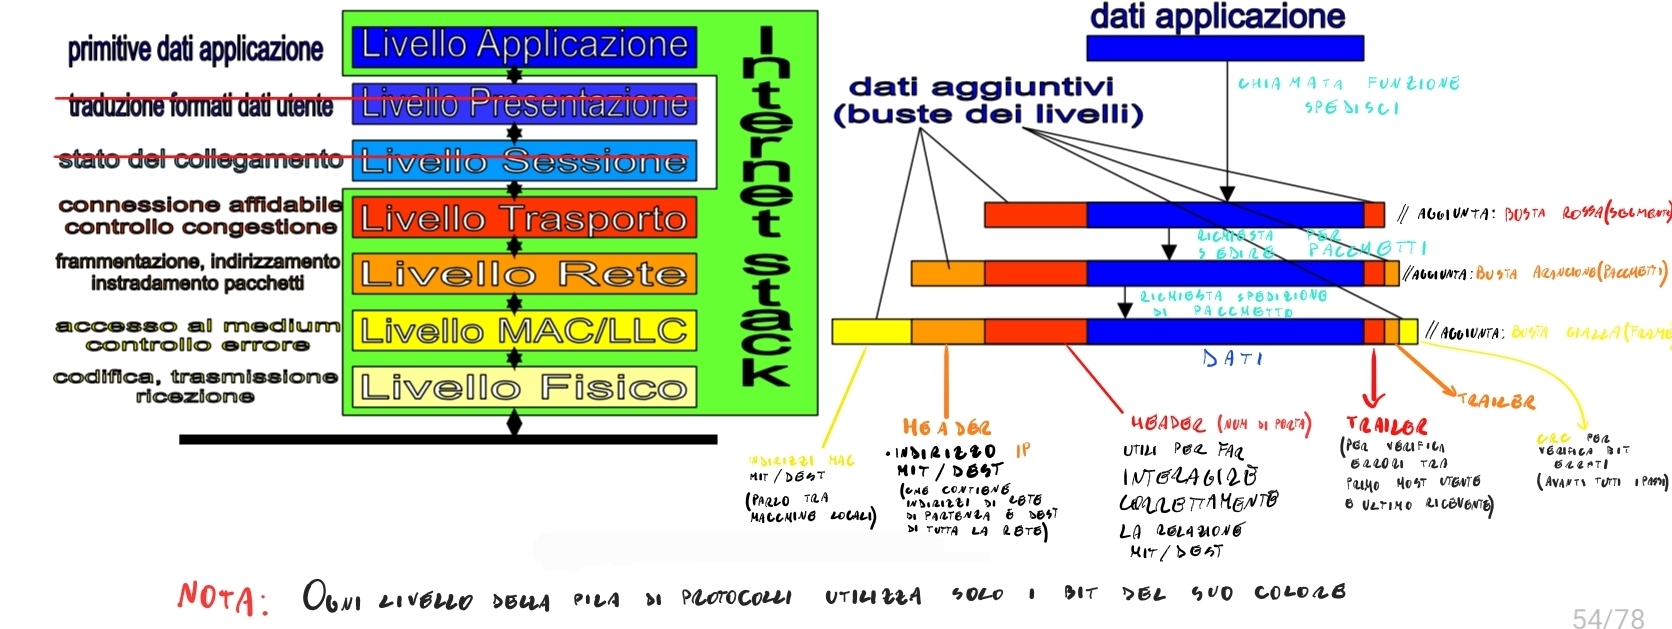
\includegraphics[width=1\linewidth]{foto reti di calcolatori/protocolli_internet.jpg}
    \caption{La pila di livelli dei protocolli di rete di internet.}
\end{figure}

\subsection*{Incapsulamento e Decapsulamento}


\begin{defbox}{Decapsulamento e incapsulamento}
L’\textbf{incapsulamento} è il processo per cui ogni livello dello stack aggiunge ai dati del livello superiore una propria \textbf{intestazione (header)} e, se necessario, un \textbf{trailer}.
Queste informazioni non fanno parte del contenuto applicativo ma servono al corretto instradamento, controllo d’integrità, sincronizzazione, segmentazione/ricomposizione e alla consegna al processo applicativo corretto.


Il \textbf{decapsulamento} è l’operazione opposta: il destinatario rimuove progressivamente header/trailer e passa il payload al livello superiore fino a tornare ai dati originali dell’applicazione.
\end{defbox}

\begin{notebox}{Comunicazione tra livelli}
È corretto dire che:
\begin{itemize}
\item ogni livello \textbf{communica logicamente} (usa protocolli) con il \textbf{livello omologo} (peer) sull'altro host — ad es. SMTP <-> SMTP, IP <-> IP, SHTP <-> SHTP;
\item \textbf{fisicamente} però i dati passano sempre tra \textbf{livelli adiacenti} all'interno dello stesso host: un livello riceve PDU (Protocol Data Unit) dal livello superiore, aggiunge il proprio header/trailer e consegna la nuova PDU al livello inferiore.
\end{itemize}
In pratica: il livello X usa solo i \textbf{bit e i campi} dell'intestazione che gli servono e \textbf{ignora} il resto.
\end{notebox}


\subsection*{ESEMPIO}
Useremo come esempio reale il protocollo di posta \textbf{SMTP} al livello applicazione (livello 7).

Per il livello trasporto, manteniamo il nome generico \textbf{SHTP} (Simple Host Transport Protocol) per evidenziare la presenza di un protocollo di trasporto che aggiunge header e trailer.
Colori usati nell’esempio:
\begin{itemize}
\item \textcolor{red}{\textbf{Busta rossa}} = PDU\footnote{Protocol Data Unit: unità di dati elaborata a ciascun livello dello stack di protocolli.}
 di trasporto (segmento SHTP);
\item \textcolor{orange}{\textbf{Busta arancione}} = PDU di rete (pacchetto IP);
\item \textcolor{yellow!80!black}{\textbf{Busta gialla}} = PDU di collegamento (frame Ethernet).
\end{itemize}

\subsection*{Incapsulamento: client SMTP $\rightarrow$ server SMTP }
\begin{enumerate}
\item \textbf{Livello 7 -- Applicazione (SMTP)}\
L’applicazione SMTP genera il messaggio (es.: \texttt{MAIL FROM:[alice@example.com](mailto:alice@example.com)} ) e lo consegna al livello trasporto. Le intestazioni applicative (From, To, Subject, MIME, ecc.) non sono header di rete ma fanno parte del payload\footnote{Payload: i dati effettivi dell’applicazione trasmessi all’interno del pacchetto, senza gli header/trailer dei livelli di rete.}
 dell’applicazione.


\item \textbf{Livello 4 -- Trasporto (SHTP)} — \textcolor{red}{\textbf{Busta rossa}}\\
SHTP incapsula il payload SMTP in un segmento e aggiunge:
\begin{itemize}
    \item \textbf{Header di trasporto}:numero di porta sorgente, porta destinazione (25 per SMTP), numero di sequenza, numero di ACK, flag di controllo (SYN/ACK/FIN).
        \item \textbf{Trailer di trasporto}: eventuali campi di controllo di fine-segmento o padding, per verificare la presenza di errori tra primo host utente e ultimo ricevente(se previsti dal protocollo).
\end{itemize}
\textbf{Scopo:} garantire consegna affidabile, ordinamento e controllo del flusso. Ogni host destinatario processerà solo l’header/trailer di trasporto quando il livello 4 del destinatario ritirerà la PDU.

\item \textbf{Livello 3 -- Rete (IP)} — \textcolor{orange}{\textbf{Busta arancione}}\\
Il segmento SHTP diventa payload del pacchetto IP; il livello 3 aggiunge:
\begin{itemize}
    \item \textbf{Header di rete}: IP sorgente, IP destinazione, campo \texttt{Protocol} (che identifica SHTP),identificatore/frammentazione.
    \item \textbf{(eventuale) Trailer di rete}: alcuni stack possono aggiungere padding o campi di allineamento; in IPv4 il checksum è generalmente nell’header.
\end{itemize}
\textbf{Scopo:} fornire informazioni logiche per l’instradamento.

\item \textbf{Livello 2 -- MAC/LLC (Ethernet)} — \textcolor{yellow!80!black}{\textbf{Busta gialla}}\\
Il pacchetto IP è incapsulato in un frame Ethernet cui vengono aggiunti:
\begin{itemize}
    \item \textbf{Header di collegamento}: MAC sorgente, MAC destinazione (del prossimo hop o host finale);
    \item \textbf{Trailer di collegamento}: CRC per il controllo d’integrità del frame sul mezzo fisico.
\end{itemize}
\textbf{Scopo:} consegna locale e rilevamento di errori sul mezzo fisico. Dispositivi di livello 2, come gli \textbf{switch}, leggono questi header per decidere la porta di uscita.

\item \textbf{Livello 1 -- Fisico}\\
Il frame viene trasformato in bit e segnali elettrici/ottici/radio e trasmesso sul mezzo.

\end{enumerate}

\begin{notebox}{Cosa succede se un livello non è il destinatario finale? (comportamento per router/switch/hub/repeater)}
\begin{itemize}
\item \textbf{Hub / Repeater (livello 1)}: si limita a rigenerare e replicare il segnale su tutte le porte; non interpreta né header né trailer; non filtra alcunché.
\item \textbf{Switch (livello 2)}: legge \textbf{solo} l’header di collegamento (indirizzi MAC) e inoltra i frame sulla porta corretta; se il MAC destinazione non è nella tabella, può inviare in broadcast sulla VLAN; non interpreta il payload IP/SHTP.
\item \textbf{Router (livello 3)}: legge \textbf{solo} l’header IP; se l’IP destinazione non è quello del router, effettua routing verso il prossimo hop (usando la tabella di routing) e ricrea un nuovo frame di livello 2 per l’interfaccia di uscita; 

se l’IP corrisponde al router, consegna il pacchetto al proprio livello 4 locale. Il router non elabora gli header di trasporto (a meno che non sia configurato per ispezione approfondita).
\item \textbf{Host destinatario}: se l’indirizzo MAC e IP coincidono con quello dell’host, il frame/pacchetto viene passato ai livelli superiori per il decapsulamento.
\end{itemize}    
\end{notebox}




\subsection*{Decapsulamento: server SMTP }
\begin{enumerate}
\item \textbf{Livello 1 -- Fisico}: i segnali sono convertiti in bit; eventuali errori fisici vengono rilevati più avanti (CRC).
\item \textbf{Livello 2 -- MAC/LLC}: il frame viene ricostruito e il trailer CRC verificato:
\begin{itemize}
\item se \textbf{CRC non valido} $\rightarrow$ frame scartato (eventuale ritrasmissione gestita dal mittente di livello 2);
\item se \textbf{CRC valido} ma MAC non corrisponde $\rightarrow$ scarto (o inoltro da switch);
\item se \textbf{MAC corrisponde} $\rightarrow$ rimozione di header e trailer di livello 2 e consegna del pacchetto IP al livello 3.
\end{itemize}
\item \textbf{Livello 3 -- Rete (IP)}: controllo dell’indirizzo IP di destinazione:
\begin{itemize}
\item se il pacchetto \textbf{non} è per questo host, il dispositivo (router) lo inoltra;
\item se \textbf{è per questo host}, l’header IP viene rimosso e il segmento SHTP viene passato al livello 4.
\end{itemize}
\item \textbf{Livello 4 -- Trasporto (SHTP)}: verifica numeri di sequenza e checksum:
\begin{itemize}
\item segmenti mancanti o corrotti $\rightarrow$ richiesta di ritrasmissione o gestione dell’errore;
\item segmenti ricevuti correttamente $\rightarrow$ invio di \textbf{ACK espliciti} (acknowledgment) al mittente e consegna del payload SMTP al livello applicazione.
\end{itemize}
\item \textbf{Livello 7 -- Applicazione (SMTP)}: il server SMTP riceve il messaggio e risponde (ad es. \texttt{250 OK}). Le risposte applicative sono poi incapsulate nuovamente per il viaggio inverso.
\end{enumerate}


\begin{notebox}{Punti chiave da evidenziare}
\begin{itemize}
\item \textbf{Transport, Network e MAC/LLC aggiungono tutti header e trailer}: header per indirizzamento/controllo, trailer generalmente per il controllo d’integrità (es. CRC).
\item \textbf{Ogni livello interpreta solo i campi che gli servono}: ad esempio, uno switch utilizza solo gli indirizzi MAC;

un router utilizza solo l’header IP; il livello trasporto utilizza solo le porte e i numeri di sequenza.
\item \textbf{Dispositivi di rete operano a livelli diversi}: hub/repeater (livello 1), switch (livello 2), router (livello 3). Questo determina quale informazione leggono e quali azioni compiono.
\item \textbf{ACK e ritrasmissione}: possono esistere acknowledgment impliciti a livello 2 (ritrasmissione sul mezzo locale se previsto) e ACK espliciti a livello di trasporto (SHTP/TCP) per garantire affidabilità end-to-end.
\end{itemize}
\end{notebox}
\vspace{3cm}



\newpage

\section{Protocolli dei lvelli ed integrazione delle reti tramite dispositivi}

Ogni livello dei protocolli di rete gestisce problematiche specifiche e aggiunge nuove funzioni di integrazione.
Dal livello fisico fino al livello applicazione, la rete evolve da un semplice collegamento tra dispositivi a un sistema globale di comunicazione tra applicazioni distribuite.

\begin{defbox}{Concetto di integrazione}
L'integrazione delle reti consiste nella capacità di interconnettere tecnologie, dispositivi e protocolli diversi in un’unica architettura coerente.
Ogni livello aggiunge regole e meccanismi che ampliano la visione della rete:
\begin{itemize}
\item il livello fisico collega dispositivi sullo stesso mezzo;
\item il livello MAC/LLC collega dispositivi in una rete locale;
\item il livello rete collega più reti tra loro;
\item il livello trasporto collega in modo affidabile le applicazioni eseguite su host remoti;
\item il livello applicazione collega gli utenti alle applicazioni.
\end{itemize}
\end{defbox}





\subsection{Livello Fisico (1)}

La rete, a questo livello, è semplicemente un \textbf{segmento fisico condiviso} con la stessa tecnologia comune per tutti i dispositivi.

\vspace{0.5cm}
\textbf{Dispositivo tipico:} \textbf{Hub} o \textbf{Repeater}.
\begin{itemize}
    \item Operano solo al livello 1: non interpretano trame, indirizzi o protocolli.
    \item Ricevono un segnale e lo rigenerano su tutte le porte.
    \item Non distinguono i destinatari: causano collisioni e condividono la banda.
    \item Se due segmenti separati sono uniti da questi, diventano uno unico.
\end{itemize}

\begin{figure}[H]
    \centering
    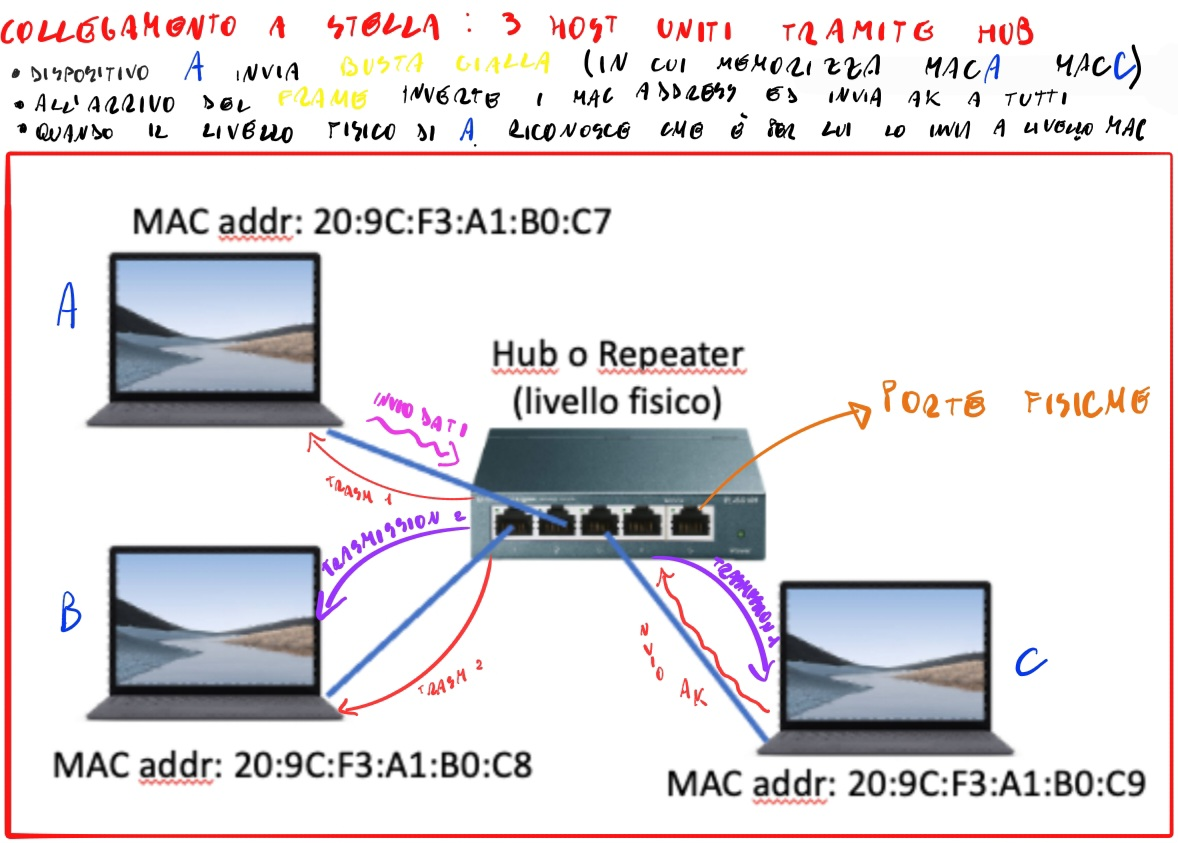
\includegraphics[width=0.6\linewidth]{foto reti di calcolatori/HUb_repeter.jpg}
    \caption{Hub/Repeater}
\end{figure}

\begin{defbox}{Repeater (Ripetitore)}
Dispositivo di \textbf{Livello 1 (Fisico)}.  
\textbf{Scopo principale:} Contrastare l'attenuazione (il degrado) del segnale elettrico/ottico per estendere la portata fisica di un singolo segmento di rete locale (ad esempio, per superare il limite fisico dei 100-200 metri dei cavi Ethernet).

\textbf{Caratteristiche chiave:}
\begin{itemize}
    \item \textbf{Rigenerazione attiva:} non si limita ad amplificare il segnale (che amplificherebbe anche il rumore), ma lo "pulisce" e lo ricostruisce perfettamente prima di ritrasmetterlo sul cavo successivo.
    \item \textbf{Invisibilità logica ("Dispositivo stupido"):} lavora esclusivamente sui bit grezzi. Non legge i frame, non sa cosa sia un indirizzo MAC o IP, e non applica alcun filtro.
    \item \textbf{Stessa tecnologia:} può collegare esclusivamente segmenti di rete che utilizzano l'identica tecnologia MAC (es. da Ethernet a Ethernet).
\end{itemize}
\end{defbox}

\begin{defbox}{Hub (Concentratore / Ripetitore multiporta)}
Dispositivo di \textbf{Livello 1 (Fisico)}, concettualmente identico a un repeater ma dotato di più porte.  
\textbf{Scopo principale:} Fungere da perno centrale per il cablaggio strutturato delle reti locali con \textbf{topologia a stella}, collegando fisicamente più dispositivi tra loro.

\textbf{Caratteristiche chiave:}
\begin{itemize}
    \item \textbf{Diffusione cieca (Broadcast fisico):} quando riceve un segnale su una porta, lo replica in modo identico e simultaneo su \textit{tutte} le altre porte attive. Tutti i dispositivi collegati ricevono fisicamente ogni trasmissione.
    \item \textbf{Dominio di collisione unico:} non filtrando né instradando i dati, si comporta come se fosse un unico cavo condiviso. Se due \textit{host} trasmettono contemporaneamente, i loro segnali si scontrano irrimediabilmente all'interno dell'Hub.
    \item \textbf{Inefficienza e obsolescenza:} ideale per le primissime e semplici reti a stella, oggi è considerato obsoleto e sostituito quasi ovunque dagli Switch (che lavorano invece al Livello 2 separando le collisioni).
\end{itemize}
\end{defbox}

\begin{notebox}{Funzione}
Gli hub e repeater servono a estendere il dominio fisico di una rete, ma non introducono alcuna intelligenza o filtraggio.
\end{notebox}

\vspace{1cm}

\subsubsection*{Codifica dei dati digitali \footnote{Vedi anche capitolo 7 parte 3 sezione 7.1.3}}

La trasmissione dei dati sul canale di comunicazione richiede un processo di \textbf{codifica} e \textbf{decodifica} dei dati da parte della scheda di rete.  
Ogni informazione digitale deve essere trasformata in un segnale analogico\footnote{%
Un \textbf{segnale analogico} è una rappresentazione continua di un’informazione, 
in cui il valore del segnale può assumere un numero infinito di stati in un intervallo di tempo. 
Esempi tipici sono i segnali elettrici, ottici o radio che variano nel tempo in modo continuo. 
A differenza dei segnali digitali, che rappresentano solo due stati (0 e 1), 
i segnali analogici devono essere \textbf{campionati e quantizzati} per poter essere elaborati o trasmessi da dispositivi digitali.}che possa viaggiare sul mezzo trasmissivo (rame, fibra ottica o onde radio).

\begin{itemize}
    \item Poiché il mezzo trasmissivo è analogico, ogni bit deve essere \textbf{codificato} in un segnale fisico (variazione di tensione, intensità luminosa o frequenza radio).
    \item La \textbf{scheda di rete} si occupa di:
    \begin{itemize}
        \item \textbf{Codificare} i bit in segnali analogici in fase di \textbf{trasmissione}.
        \item \textbf{Decodificare} i segnali ricevuti per ricostruire i bit originali, in fase di \textbf{ricezione}.
    \end{itemize}
    \item Le tecniche di codifica digitali permettono di ridurre, ma non eliminare completamente, gli errori di trasmissione.
\end{itemize}

\begin{notebox}{Velocità e capacità del canale}
È importante distinguere tra:
\begin{itemize}
    \item La \textbf{velocità di propagazione} dei segnali, che è fisicamente la stessa per tutti i mezzi trasmissivi (pari alla velocità della luce, circa 300.000 km/s).
    \item La \textbf{capacità del canale di trasmissione}, ovvero il numero massimo di bit che possono essere trasmessi ogni secondo (\textbf{bit/s}).
\end{itemize}

Tutti i segnali, elettrici, ottici o radio, si propagano quasi alla stessa velocità fisica, ma i canali possono differire per la \textbf{densità di trasmissione dei bit}, cioè per quanti bit riescono a codificare per unità di tempo.

Ad esempio, un canale in grado di rappresentare un bit ogni microsecondo ha capacità doppia rispetto a uno che impiega due microsecondi per codificare lo stesso bit.
\end{notebox}

\begin{esempiobox}{Confronto tra due canali digitali}
Si considerino due canali digitali, \textbf{A} (rosso) e \textbf{B} (giallo):

\begin{itemize}
    \item Entrambi propagano i segnali alla stessa velocità fisica (velocità della luce).
    \item Tuttavia, il canale \textbf{B} riesce a \textbf{codificare un bit in metà tempo} rispetto al canale \textbf{A}.
    \item Di conseguenza, la \textbf{capacità di trasmissione} (bit/s) del canale B è il doppio di quella del canale A.
\end{itemize}

\textbf{Interpretazione:}
\begin{itemize}
    \item\textbf{ Non esistono “bit più veloci”, ma canali con capacità maggiore perché riescono a rappresentare i bit in tempi più brevi.}
    \item Le migliori tecnologie di rete sono quelle che permettono di codificare i bit nel minor tempo possibile, raggiungendo così capacità elevate (fino a miliardi di bit al secondo).
\end{itemize}
\end{esempiobox}

\begin{figure}[H]
    \centering
    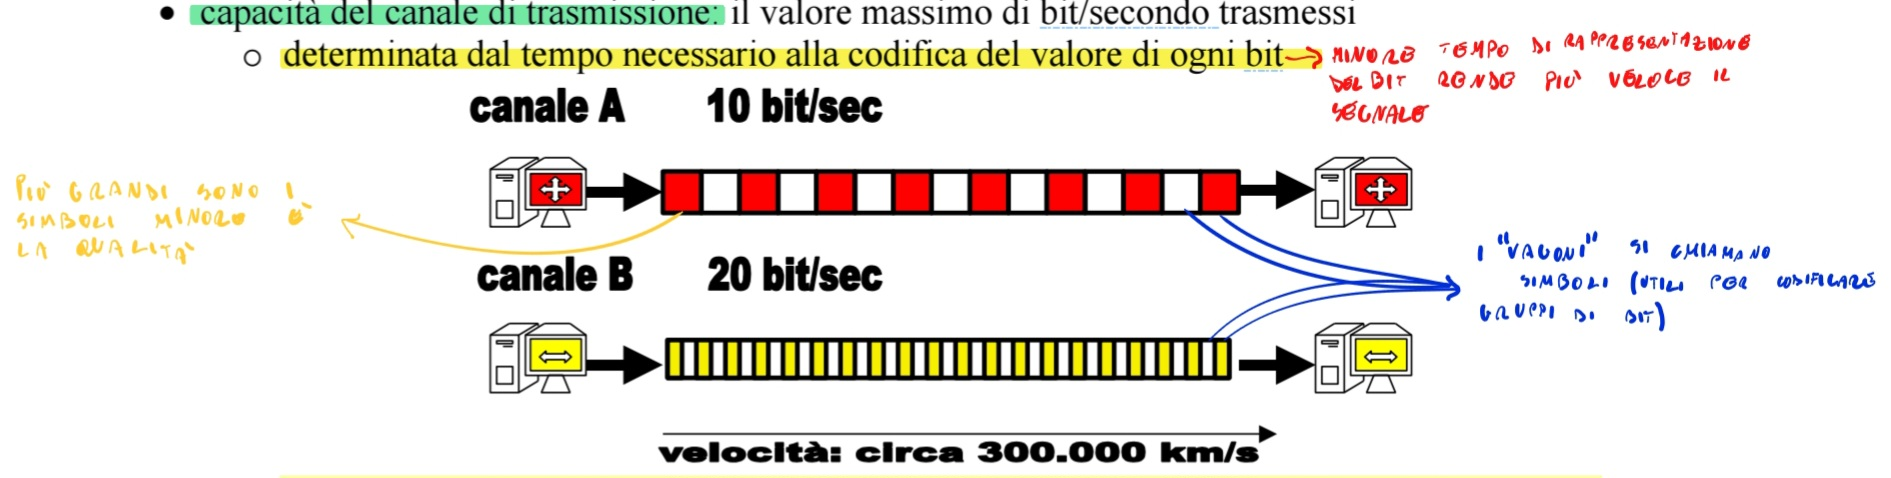
\includegraphics[width=1\linewidth]{foto reti di calcolatori/canali_digitali.jpg}
    \caption{Esempio di due canali digitali con diversa capacità di trasmissione}
\end{figure}



\newpage
\subsection{Livello MAC/LLC (Collegamento Dati)}
A questo livello, la rete diventa \textbf{una LAN (Local Area Network)}.
\vspace{0.5cm}

\textbf{Dispositivo tipico:} \textcolor{yellow!80!black}{Switch o bridge}.
\begin{itemize}
\item Legge gli \textbf{header e trailer del frame},\textcolor{yellow!80!black}{Busta gialla};
\item individua il MAC di destinazione e inoltra il frame solo sulla porta corretta;
\item isola le collisioni creando \textbf{domini di collisione distinti};
\item mantiene una \textbf{tabella MAC} (indirizzo–porta) aggiornata dinamicamente.
\end{itemize}

\begin{defbox}{Bridge (Ponte)}
Dispositivo di \textbf{Livello 2 (MAC/LLC)}.  
\textbf{Scopo principale:} Connettere tra loro due (o pochissimi) segmenti di rete locale che utilizzano \textbf{tecnologie MAC differenti} (es. unisce un segmento Ethernet a uno Token Ring).  

\textbf{Caratteristiche chiave:}
\begin{itemize}
    \item \textbf{Agisce da traduttore:} riceve un frame, ne adatta l'intestazione e il formato alla tecnologia del segmento di destinazione e lo ritrasmette.
    \item \textbf{Filtra il traffico:} inoltra i frame solo se il destinatario si trova effettivamente sull'altro segmento, impedendo al traffico inutile di intasare l'altra rete.
    \item Tipicamente è dotato di sole \textbf{due porte} fisiche (una per ogni rete da connettere).
\end{itemize}
\end{defbox}

\begin{defbox}{Switch (Commutatore multiporta)}
Dispositivo di \textbf{Livello 2 (MAC/LLC)}, nato come evoluzione diretta del bridge.  
\textbf{Scopo principale:} Connettere un elevato numero di calcolatori o segmenti che utilizzano tutti la \textbf{stessa tecnologia} (oggi standard per le LAN Ethernet a stella).  

\textbf{Caratteristiche chiave:}
\begin{itemize}
    \item \textbf{Inoltro selettivo:} legge l'indirizzo MAC di destinazione e invia il frame \textit{esclusivamente} sulla porta a cui è collegato il destinatario, ignorando le altre.
    \item \textbf{Micro-segmentazione:} crea dei circuiti virtuali punto-a-punto temporanei tra chi spedisce e chi riceve. Permette a più coppie di computer di parlarsi contemporaneamente \textbf{azzerando il rischio di collisioni}.
    \item È dotato di \textbf{molte porte} (es. 8, 24 o 48), agendo come il vero e proprio "vigile urbano" del traffico locale.
\end{itemize}
\end{defbox}

\begin{notebox}{Ruolo dell’header e del trailer}
\textbf{Header MAC}: contiene indirizzi sorgente e destinazione e tipo di protocollo.

\textbf{Trailer CRC}: controlla l’integrità del frame.
Sono usati solo dagli switch e scartati dai livelli superiori.
\end{notebox}

\begin{defbox}{Tipologie di Switch}
Esistono due principali tipologie di switch di rete:

\begin{itemize}
    \item \textbf{Switch unmanaged:} sono dispositivi \textit{plug-and-play}, ovvero non richiedono alcuna configurazione. 
    Gestiscono automaticamente il traffico tra i dispositivi collegati, ma non permettono di monitorare o controllare le connessioni. 
    Sono usati tipicamente in piccole reti domestiche o uffici dove non è necessario un controllo avanzato.

    \item \textbf{Switch managed:} consentono la \textit{configurazione, il monitoraggio e la gestione} del traffico di rete. Contengono al loro interno più livelli ed 
    offrono funzionalità avanzate come QoS (Quality of Service), sicurezza, ridondanza e gestione remota tramite interfaccia web o riga di comando.
    Sono ideali per reti aziendali o ambienti complessi che richiedono controllo e affidabilità.
\end{itemize}
\end{defbox}

\subsubsection*{ Collegamento con Switch (livello MAC/LLC)}
\begin{figure}[H]
    \centering
    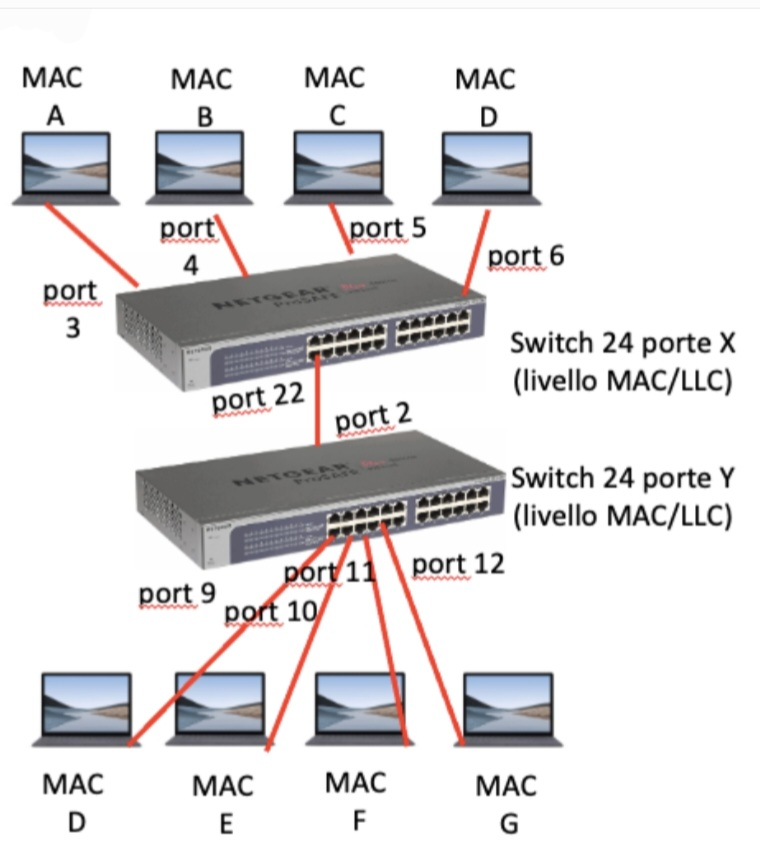
\includegraphics[width=0.5\linewidth]{foto reti di calcolatori/switch_es.jpg}
    \caption{Switch}
    \label{fig:switch}
\end{figure}


Nella figura ~\ref{fig:switch} sono rappresentati due switch (\textbf{Switch X} e \textbf{Switch Y}) collegati tra loro.  
Gli host A, B, C e D sono connessi allo switch X, mentre gli host D, E, F e G sono connessi allo switch Y.  
Le due reti locali (LAN) sono interconnesse tramite una \textbf{porta di uplink} (porta 22 dello switch X connessa alla porta 2 dello switch Y).

\textbf{Funzionamento:}
\begin{itemize}
    \item Gli switch operano al \textbf{livello 2 (MAC/LLC)}.
    \item Mantengono una \textbf{tabella di associazione MAC ↔ porta} che permette di inoltrare i frame solo sulla porta corretta.
    \item Se un MAC non è ancora noto, lo switch esegue un \textit{flooding}, cioè invia il frame su tutte le porte tranne quella d’origine.
    \item Ogni porta crea un \textbf{dominio di collisione separato} (in caso più host volessero parlare contemporaneamente), migliorando efficienza e prestazioni.
\end{itemize}



\begin{notebox}{\textbf{Criticità Architetturali: Uplink e Domini}}
Collegare due switch in cascata (tramite una singola porta di \textit{uplink}, come le porte 22 e 2) risolve il problema delle distanze e del numero di porte, ma introduce tre criticità fondamentali:

\begin{itemize}[leftmargin=*]
    \item \textbf{Collo di bottiglia (Bottleneck) sull'Uplink:} 
    Il singolo cavo che unisce lo Switch X allo Switch Y deve farsi carico dell'intero traffico scambiato tra le due metà della rete. Se gli host A, B e C decidono di trasferire grossi file contemporaneamente verso gli host E, F e G, il cavo di uplink si saturerà rapidamente, rallentando tutti. 
    \textit{(Soluzione tipica: le porte di uplink vengono progettate per essere molto più veloci delle porte normali, ad esempio a 10 Gbps o 40 Gbps, oppure si aggregano più cavi fisici).}

    \item \textbf{Single Point of Failure (Punto critico di guasto):} 
    Esattamente come nell'esempio con l'Hub (vedi pagina a seguire), non c'è ridondanza. Se il cavo di uplink si danneggia o una delle due porte si brucia, la rete subisce un \textbf{partizionamento}: gli host sopra non potranno più parlare con gli host sotto.

    \item \textbf{Unico grande Dominio di Broadcast:} 
    Lo switch separa egregiamente i \textbf{domini di collisione} (ogni porta è un "tubo" privato, quindi niente scontri elettrici), ma l'intera rete rimane un unico \textbf{dominio di broadcast}. Se un nodo invia un pacchetto a "tutti" (indirizzo broadcast, es. protocollo ARP), o se lo switch deve fare \textit{flooding} per un MAC che non conosce, quel pacchetto attraverserà l'uplink e "inonderà" inutilmente anche tutte le porte del secondo switch, sprecando banda.
\end{itemize}
\end{notebox}
\begin{esempiobox}{Invio di un frame e ACK di ritorno}
Supponiamo che l’host \textbf{A} voglia inviare un frame all’host \textbf{E}.  
Il funzionamento procede come segue:

\begin{enumerate}
    \item \textbf{A} prepara un frame con indirizzo MAC di destinazione = MAC\textsubscript{E} e lo invia allo \textbf{Switch X}.
    \item Lo \textbf{Switch X}, non conoscendo ancora la porta associata a MAC\textsubscript{E}, effettua un \textbf{flooding}: inoltra il frame su tutte le porte tranne quella d’origine.
    \item Il frame raggiunge la porta di \textbf{uplink} e viene inviato allo \textbf{Switch Y}.
    \item Lo \textbf{Switch Y} riceve il frame, verifica che MAC\textsubscript{E} è collegato alla propria porta 10 e inoltra il frame solo su quella porta.
    \item L’host \textbf{E} riceve il frame e invia un \textbf{ACK (acknowledgment)} a \textbf{A} come conferma della ricezione.
    \item Durante il ritorno dell’ACK, gli switch aggiornano le loro \textbf{tabelle MAC}:
    \begin{itemize}
        \item Switch Y memorizza che MAC\textsubscript{A} si trova sulla porta di uplink.
        \item Switch X memorizza che MAC\textsubscript{E} è raggiungibile tramite la porta di uplink.
    \end{itemize}
    Da questo momento, i frame successivi tra A ed E saranno inoltrati direttamente, senza flooding.
\end{enumerate}
\end{esempiobox}


\newpage
\subsubsection{\textbf{Analisi di un errore progettuale: Switch + Hub}}
\begin{figure}[H]
    \centering
    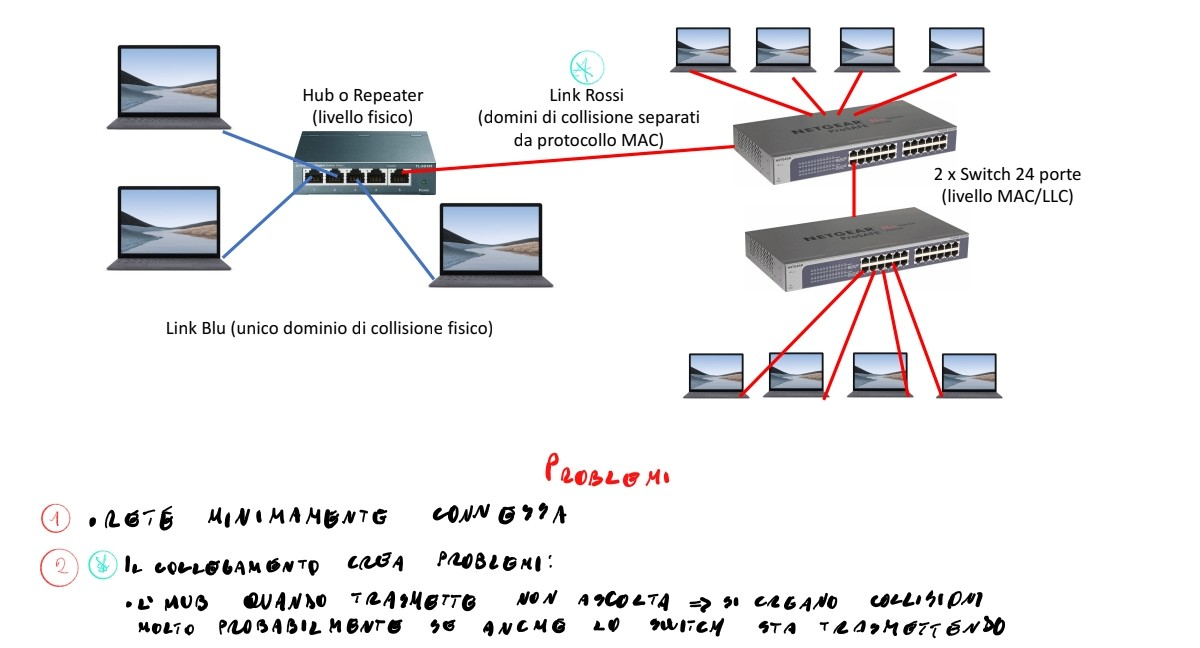
\includegraphics[width=0.9\linewidth]{foto reti di calcolatori/esempio_nonfunz.jpg}
    \caption{Esempio rete che  non funziona : switch + hub}
\end{figure}

\begin{notebox}{}
Unire dispositivi di livello diverso senza le dovute precauzioni può compromettere l'efficienza della rete. Collegando un \textbf{Hub} a uno \textbf{Switch} si va incontro a due problematiche principali:

\begin{itemize}[leftmargin=*]
    \item \textbf{1. Rete minimamente connessa (Assenza di ridondanza):}
    L'intera infrastruttura dipende dal singolo collegamento (link) tra l'Hub e lo Switch. Questo crea un \textit{Single Point of Failure}: la rottura di quel cavo, o il guasto dell'Hub stesso, provoca il partizionamento della rete, isolando un intero gruppo di macchine.

    \item \textbf{2. Collisioni sul collegamento principale (Bottleneck):}
    Il problema più grave deriva dalla natura hardware dell'Hub.
    \begin{itemize}
        \item L'\textbf{Hub} (Livello Fisico) non possiede memoria (buffer) e \textbf{non ascolta} il canale prima di trasmettere. Si limita a replicare ciecamente i segnali elettrici.
        \item Se un PC collegato all'Hub inizia a trasmettere, l'Hub propaga istantaneamente il segnale anche verso lo Switch.
        \item Se, in quell'esatto millisecondo, lo \textbf{Switch} sta inoltrando un pacchetto verso l'Hub, i due segnali viaggiano in direzioni opposte sullo stesso filo e si schiantano, generando una \textbf{collisione} che corrompe i dati.
        \item Poiché l'Hub costringe quel segmento a operare in \textit{Half-Duplex} (si parla uno alla volta) ma non gestisce le code, le collisioni diventano molto probabili, obbligando i nodi a continue ritrasmissioni e facendo crollare le prestazioni.
    \end{itemize}
\end{itemize}
\end{notebox}

\newpage
\subsection{Livello Rete}
A questo livello, la rete diventa una \textbf{collezione di reti} — una struttura gerarchica di sottoreti interconnesse.
\vspace{0.5cm}

\textbf{Dispositivo tipico:} \textcolor{orange!80!black}{Router}
\begin{itemize}  
\item Legge gli \textbf{header e trailer del pacchetto},\textcolor{orange!80!black}{Busta arancione };
\item decide l’instradamento del pacchetto in base alla tabella di routing;
\item scarta pacchetti non destinati alla propria rete o TTL scaduto.
\end{itemize}

\begin{notebox}{Header e trailer al livello rete}
\textbf{Header IP}: include indirizzi IP sorgente/destinazione.
Solo il router lo interpreta; gli switch e gli hub lo vedono come semplice payload.
\end{notebox}


\begin{figure}[H]
    \centering
    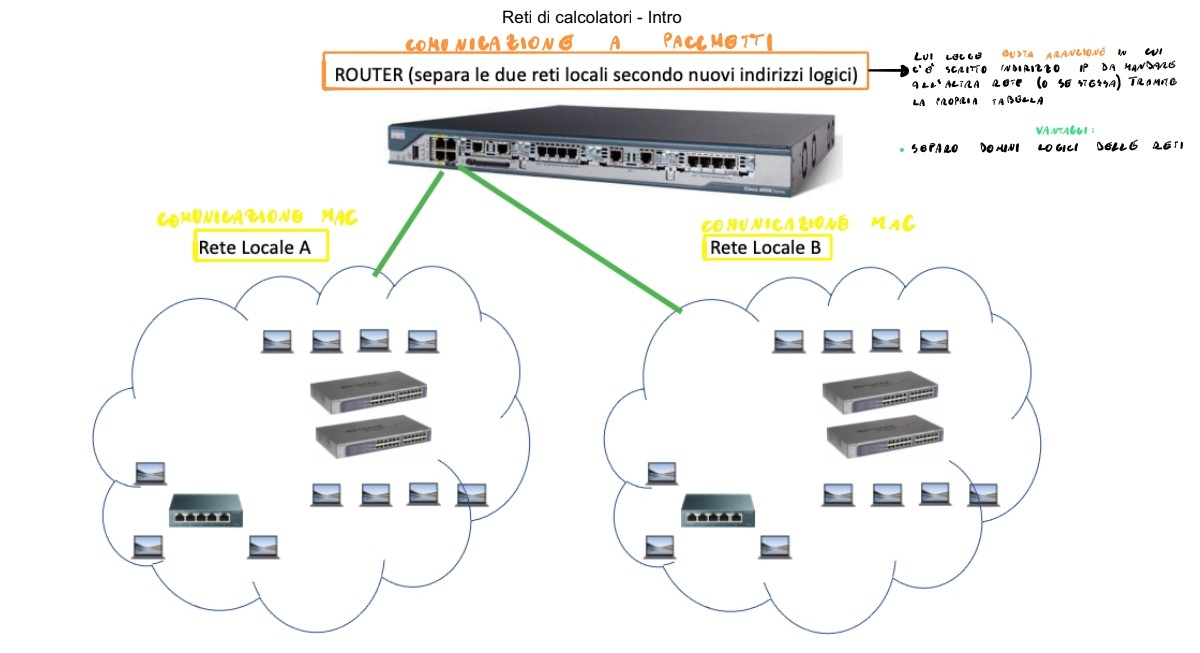
\includegraphics[width=0.9\linewidth]{foto reti di calcolatori/router_es.jpg}
    \caption{Router}
\end{figure}

\newpage 
\subsection{Livello Trasporto}
La rete, a questo livello, è una \textbf{collezione di reti interconnesse}, orientate alla connessione, vista come un’unica infrastruttura.
Il livello trasporto (es. SHTP o TCP) garantisce:
\begin{itemize}
\item la \textbf{consegna affidabile} dei segmenti (ACK, ritrasmissione);
\item il \textbf{controllo della congestione} e della velocità;
\item la \textbf{gestione delle porte} (multiplexing/demultiplexing);
\item l’\textbf{ordinamento dei dati}.
\end{itemize}

\begin{notebox}{Header e trailer di trasporto}
\textbf{Header}: contiene numero porte sorgente/destinazione, numeri di sequenza, flag (SYN, ACK, FIN), checksum.
\textbf{Trailer}: eventuale controllo di errore a livello segmento.
Solo il livello trasporto interpreta questi campi: router e switch lo trattano come payload.
\end{notebox}

\subsection{Livello Applicazione}
A questo livello, la rete “esiste” e diventa \textbf{utilizzabile dalle applicazioni utente}.
Esempi di protocolli:
\begin{itemize}
\item SMTP (posta elettronica),
\item HTTP/HTTPS (web),
\item DNS (risoluzione nomi),
\item FTP, SSH, ecc.
\end{itemize}
Il protocollo applicativo genera dati che saranno incapsulati dai livelli inferiori.

\subsection*{Dispositivi di Rete: confronto}

\begin{center}
\begin{tabular}{|c|c|c|c|}
\hline
Dispositivo & Livello OSI & Dominio di Collisione & Dominio di Broadcast \\
\hline
Hub & 1 & Unico & Unico \\
Switch & 2 & Uno per porta & Unico \\
Router & 3 & Uno per porta & Uno per porta \\
\hline
\end{tabular}
\end{center}

\begin{notebox}{Conclusione}
Lo Switch migliora l'efficienza della LAN, il Router permette di comunicare con altre reti e filtrare il traffico.
\end{notebox}


\newpage
\subsection{Parentesi sull'affidabilità della comunicazione in rete}
\begin{figure}[H]
    \centering
    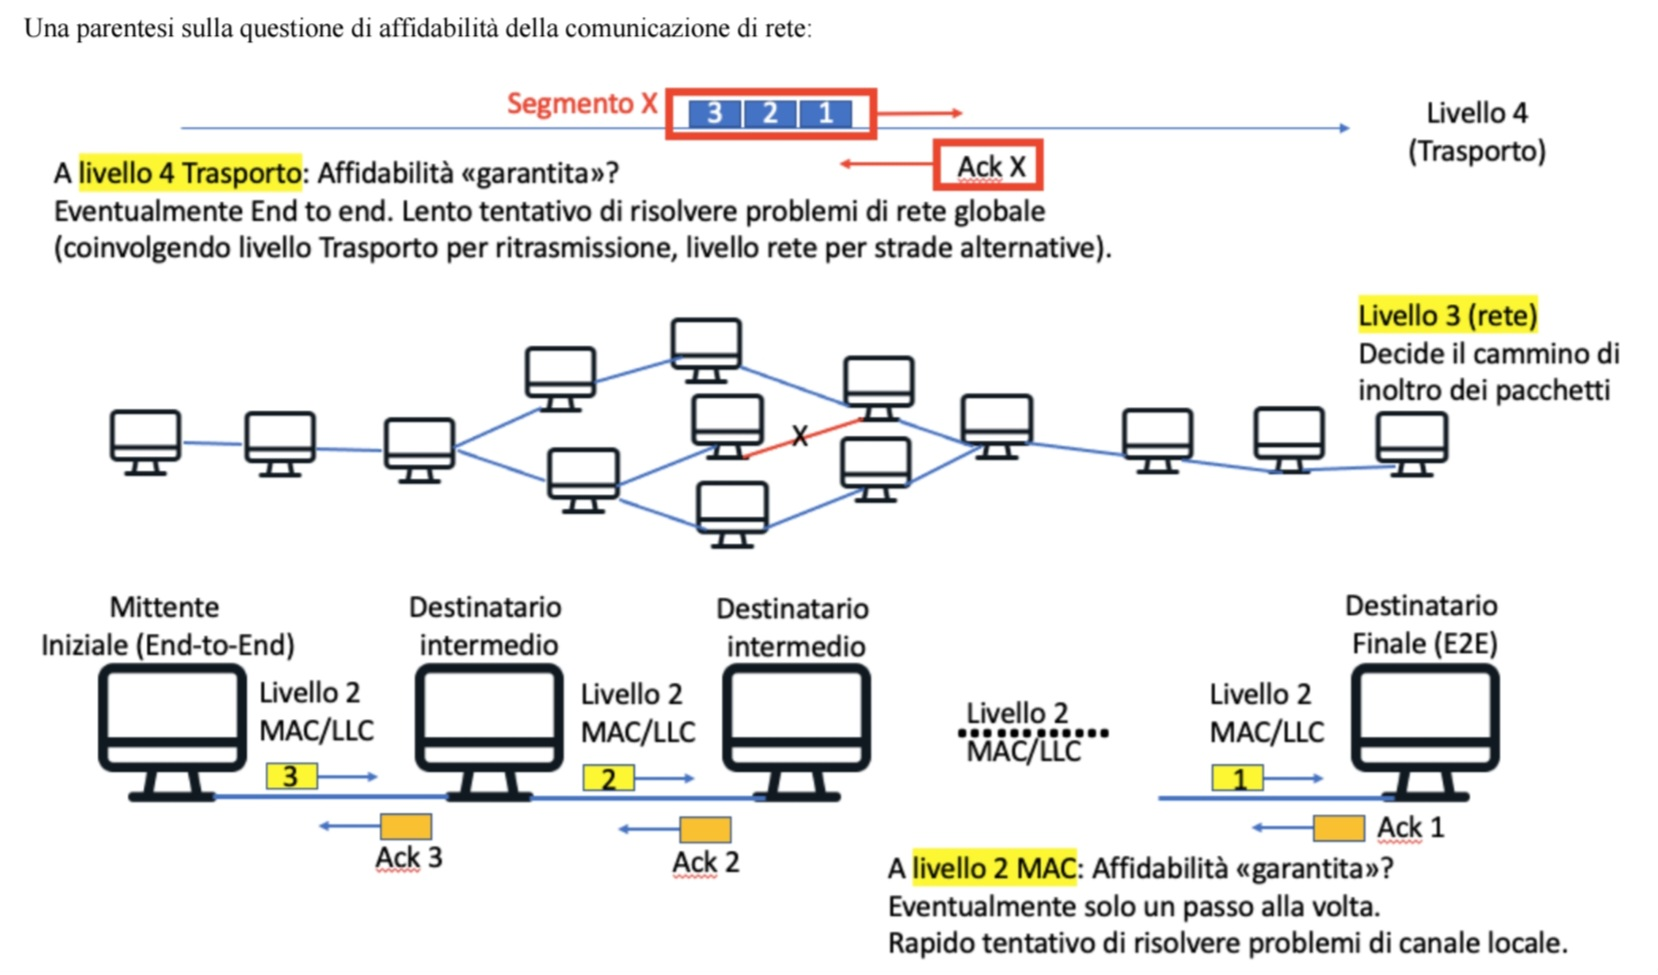
\includegraphics[width=\textwidth]{foto reti di calcolatori/affidabilita.jpg}
    \caption{Confronto sulla gestione dell'affidabilità ai vari livelli del modello OSI. Viene evidenziata la differenza tra il controllo "hop-by-hop" (rapido e locale) del Livello 2 e il controllo "end-to-end" (lento e globale) del Livello 4.}
    \label{fig:affidabilita_reti}
\end{figure}

\noindent
L'immagine in Figura~\ref{fig:affidabilita_reti} illustra come diversi livelli della pila protocollare collaborino per garantire la consegna dei dati, operando su scale spaziali e temporali differenti:

\vspace{0.3cm}

\begin{tcolorbox}[colback=red!5!white, colframe=red!70!black, title=\textbf{Livello 4 -- Trasporto (Controllo Globale)}]
\begin{itemize}[leftmargin=*]
    \item \textbf{Affidabilità End-to-End:} La comunicazione avviene esclusivamente tra il mittente iniziale e il destinatario finale, ignorando completamente tutti i router o gli switch intermedi.
    \item \textbf{Risoluzione "Lenta":} Il tentativo di recuperare un errore è lento perché agisce su scala globale. Se un pacchetto viene perso a metà strada, il mittente originale se ne accorge solo dopo lo scadere di un lungo \textit{timeout} e deve ritrasmettere il dato riattraversando l'intera rete.
    \item \textbf{Esempio pratico:} Il protocollo TCP garantisce che tutti i segmenti (es. Segmento X) arrivino a destinazione nell'ordine corretto tramite meccanismi di \texttt{ACK} globali.
\end{itemize}
\end{tcolorbox}

\begin{tcolorbox}[colback=orange!5!white, colframe=orange!90!black, title=\textbf{Livello 3 -- Rete (Instradamento)}]
\begin{itemize}[leftmargin=*]
    \item \textbf{Scelta del cammino (\textit{Routing}):} Non si occupa direttamente di ritrasmettere i dati persi, ma ha il compito cruciale di decidere il percorso migliore (\textit{best effort}) per inoltrare i pacchetti da un capo all'altro della rete.
    \item \textbf{Adattamento ai guasti:} Come evidenziato dalla "X" rossa nel diagramma, se un collegamento fisico si interrompe, i protocolli di routing del Livello 3 ricalcolano dinamicamente una \textbf{strada alternativa} per aggirare l'ostacolo.
\end{itemize}
\end{tcolorbox}

\begin{tcolorbox}[colback=yellow!3!white, colframe=yellow!80!black, title=\textbf{Livello 2 -- MAC/LLC (Controllo Locale)}]
\begin{itemize}[leftmargin=*]
    \item \textbf{Affidabilità "Hop-by-Hop" (un passo alla volta):} La garanzia di consegna avviene solo localmente, ovvero tra due nodi fisicamente adiacenti collegati dallo stesso mezzo trasmissivo.
    \item \textbf{Risoluzione "Rapida":} Il controllo è estremamente veloce. Se c'è un'interferenza sul cavo locale, il nodo intermedio non riceve l'\texttt{ACK} locale e ritrasmette \textit{immediatamente} il \textit{frame} solo su quel singolo tratto, senza scomodare il mittente originale (Livello 4) e senza intasare il resto della rete.
\end{itemize}
\end{tcolorbox}

\bigskip
\noindent
\textbf{In sintesi:}
\begin{itemize}
    \item Il \textbf{Livello 2} corregge tempestivamente gli errori fisici \textit{locali} (su ogni singolo salto).
    \item Il \textbf{Livello 3} garantisce che esista sempre un \textit{percorso} valido aggirando i link interrotti.
    \item Il \textbf{Livello 4} fornisce la garanzia assoluta e \textit{globale} che il dato sia arrivato integro e in ordine all'applicazione finale.
\end{itemize}





\newpage
\section{Livello MAC (2): tecnologie per schede di rete}

Esistono diverse tecnologie di livello MAC che possono essere usate per collegare calcolatori in reti locali. La scelta di una tecnologia stabilisce il tipo di schede di rete richieste, la topologia e il modo in cui viene regolato l'accesso al mezzo di trasmissione.

\subsection{Protocollo Ethernet}

Ethernet è il protocollo MAC in assoluto più diffuso nelle reti locali cablate. Storicamente, per gestire l'accesso al mezzo condiviso ed evitare il caos, utilizza il meccanismo \textbf{CSMA/CD} (\textit{Carrier Sense Multiple Access with Collision Detection}), che si basa sui seguenti principi:

\begin{itemize}[leftmargin=*]
    \item \textbf{Ascolto preventivo (\textit{Carrier Sense}):} Le schede di rete "ascoltano" il canale prima di agire. Se rilevano che nessuno sta trasmettendo, avviano la trasmissione.
    \item \textbf{Rilevamento delle collisioni (\textit{Collision Detection}):} Se due dispositivi iniziano a trasmettere nello stesso istante (o prima che il segnale dell'altro faccia in tempo a raggiungerli), i segnali elettrici si sovrappongono e si corrompono. Le schede di rete trasmittenti sono in grado di accorgersi di questa \textbf{collisione} in tempo reale, mentre stanno trasmettendo.
    \item \textbf{Interruzione e Attesa casuale:} Appena rilevata la collisione, la trasmissione viene interrotta immediatamente per non sprecare banda. Per risolvere l'ingorgo, ogni nodo coinvolto genera un "tempo di ritardo da scontare": pesca un intervallo di attesa \textbf{casuale} e aspetta in silenzio prima di riprovare.
    \item \textbf{Backoff Esponenziale (Potenze di due):} Se anche al secondo tentativo si verifica una nuova collisione, la finestra temporale da cui i dispositivi "pescano" il numero casuale viene \textbf{raddoppiata} (cresce per potenze di due). Questo meccanismo "spalma" statisticamente i tentativi nel tempo, riducendo drasticamente la probabilità che i due PC peschino nuovamente lo stesso ritardo.
\end{itemize}

\begin{notebox}{\textbf{Evoluzione moderna}}
Nelle moderne LAN cablate, strutturate con topologia a stella e basate su \textbf{Switch} (anziché Hub), i domini di collisione sono fisicamente separati per ogni porta. In questi scenari, il problema delle collisioni è praticamente eliminato alla radice.
\end{notebox}

\begin{figure}[H]
    \centering
     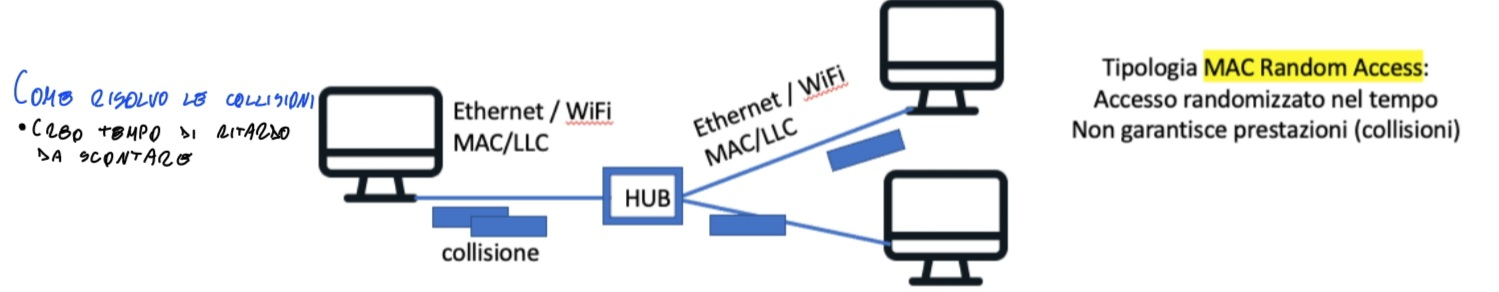
\includegraphics[width=0.9\linewidth]{foto reti di calcolatori/Ethernet.jpg}
    \caption{\textbf{Topologia MAC Random Access:} L'immagine illustra il problema dell'accesso casuale su un mezzo condiviso (es. un Hub). Due host trasmettono simultaneamente generando una collisione. Come annotato, il conflitto si risolve imponendo un "tempo di ritardo da scontare" prima della ritrasmissione. Questo approccio randomizzato è semplice ma \textit{non garantisce prestazioni costanti}, poiché l'attesa è imprevedibile.}
    \label{fig:ethernet_collision}
\end{figure}

\newpage
\subsection{Protocollo IEEE 802.11 (Wi-Fi)}

Lo standard IEEE 802.11 definisce il funzionamento delle reti locali senza fili.

\begin{itemize}
    \item Prima di trasmettere la scheda verifica che il canale sia libero, come in Ethernet.
    \item Nel wireless non è possibile rilevare una collisione durante la trasmissione, quindi si tenta di \textbf{evitarla} introducendo attese casuali prima dell'accesso al canale.
    \item Il protocollo regola i tempi di accesso in modo da ridurre la probabilità che due dispositivi trasmettano nello stesso istante.
\end{itemize}


Lo standard utilizza CSMA/CA (Collision Avoidance) a causa dei limiti fisici del mezzo wireless.

\subsection{Protocollo Token Ring}

Token Ring è una tecnologia MAC progettata per reti cablate a topologia ad anello.

\begin{itemize}
    \item Un frame speciale, detto \textbf{token}, viene passato tra i dispositivi della rete.
    \item Solo chi possiede il token può trasmettere.
    \item Terminata la trasmissione, il token viene passato al nodo successivo.
\end{itemize}

Il meccanismo di accesso permette di evitare collisioni sul canale.  
La tecnologia ha oggi un utilizzo marginale rispetto a Ethernet.

\begin{figure}[H]
    \centering
    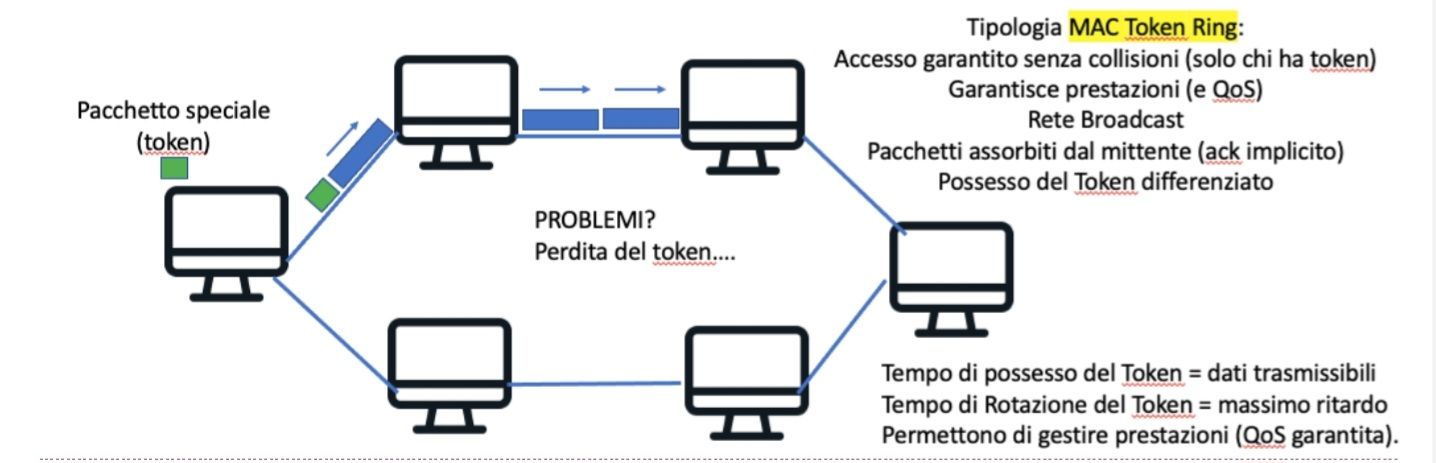
\includegraphics[width=0.9\linewidth]{foto reti di calcolatori/Token_ring.jpg}
    \caption{}
\end{figure}

\subsection*{Confronto sintetico}

\begin{center}
\begin{tabular}{|c|c|c|c|}
\hline
\textbf{Tecnologia} & \textbf{Mezzo} & \textbf{Accesso al canale} & \textbf{Collisioni} \\
\hline
Ethernet & Cablato & CSMA/CD & Possibili (evitate con switch) \\
\hline
IEEE 802.11 & Wireless & CSMA/CA & Evitate per prevenzione \\
\hline
Token Ring & Anello cablato & Token passing & Assenti \\
\hline
\end{tabular}
\end{center}






\newpage
\section*{Esempi di Rete a Commutazione di Pacchetto}

\subsection{Segmento di Rete Locale e affidabilità livello MAC}

Il \textbf{segmento di rete locale} rappresenta il livello più semplice di una rete a \textbf{commutazione di pacchetto}.  
In questo contesto, tutti i dispositivi condividono lo stesso mezzo trasmissivo e accedono al canale tramite un \textbf{canale ad accesso multiplo}.

\begin{itemize}
    \item Tutte le \textbf{schede di rete} collegate ricevono ogni trasmissione effettuata sul mezzo trasmissivo.
    \item Ogni scheda possiede un \textbf{indirizzo fisico univoco} (indirizzo MAC), assegnato dal produttore.
    \item Il canale condiviso è di tipo \textbf{broadcast}: un frame trasmesso è visibile da tutti i nodi della rete locale.
\end{itemize}

\begin{figure}[H]
    \centering
    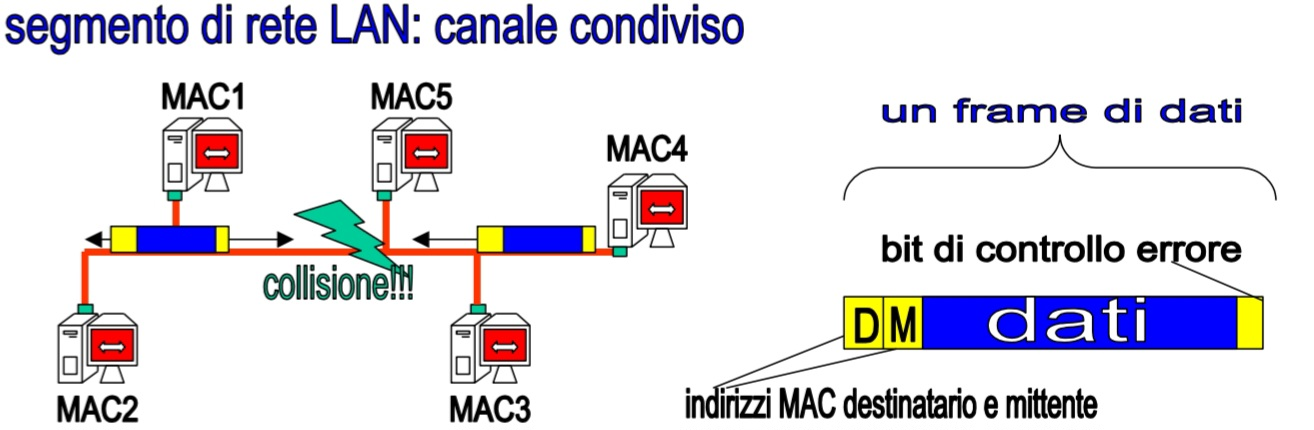
\includegraphics[width=0.7\linewidth]{foto reti di calcolatori/segmento_locale.jpg}
    \caption{Esempio di rete locale con canale condiviso e 5 dispositivi con indirizzi MAC diversi}
\end{figure}

\begin{esempiobox}{Trasmissione su canale condiviso}
Immaginiamo una rete locale composta da cinque dispositivi, ciascuno con un indirizzo MAC univoco.  
Supponiamo che:
\begin{itemize}
    \item Il dispositivo con indirizzo \textbf{MAC1} voglia inviare un frame a \textbf{MAC5}.
    \item Contemporaneamente, \textbf{MAC4} voglia inviare un frame a \textbf{MAC2}.
\end{itemize}

Poiché il mezzo è condiviso, entrambe le trasmissioni viaggiano sullo stesso canale fisico.  
Se i due dispositivi trasmettono nello stesso istante, i segnali si \textbf{sovrappongono}, generando una \textbf{collisione distruttiva}.  
Il risultato è la perdita di entrambe le trasmissioni.
\end{esempiobox}

\newpage

\subsubsection*{Affidabilità sul canale condiviso}

Scopo dei protocolli MAC/LLC è rendere il canale condiviso \textbf{affidabile}, compensando gli errori dovuti a collisioni o interferenze.

\begin{itemize}
    \item Dopo la trasmissione di un frame, il mittente attende una \textbf{conferma di ricezione (ACK)} dal destinatario.
    \item Se la conferma non arriva entro un certo tempo, il frame viene ritrasmesso.
    \item Il processo continua fino alla ricezione positiva della conferma.
\end{itemize}


\begin{esempiobox}{Trasmissione affidabile tra due dispositivi}
Supponiamo che \textbf{MAC1} invii un frame a \textbf{MAC2}.  
La sequenza temporale può essere la seguente:
\begin{enumerate}
    \item MAC1 trasmette il frame e avvia un timer.
    \item MAC2 riceve il frame ma rileva un errore nei bit, quindi lo scarta e non invia conferma.
    \item Allo scadere del timer, MAC1 ritrasmette il frame.
    \item MAC2 riceve correttamente il frame e invia un \textbf{frame di conferma (ACK)} a MAC1.
    \item MAC1 riceve l’ACK e considera conclusa con successo la trasmissione.
\end{enumerate}
\end{esempiobox}

un'altra tecnica utilizzata per risolvere il problema della condivisione contemporanea è quella di \textbf{eleggere un rappresentante} che abbia priorità maggiore

\begin{notebox}{Obiettivo del livello MAC/LLC}
Lo scopo principale del livello 2 è \textbf{nascondere ai livelli superiori} i dettagli fisici e le problematiche del mezzo trasmissivo,  
presentando un canale logico \textbf{affidabile e privo di errori}.  
In questo modo, i protocolli dei livelli superiori possono comunicare come se il mezzo fosse perfetto.
\end{notebox}

\begin{figure}[H]
    \centering
    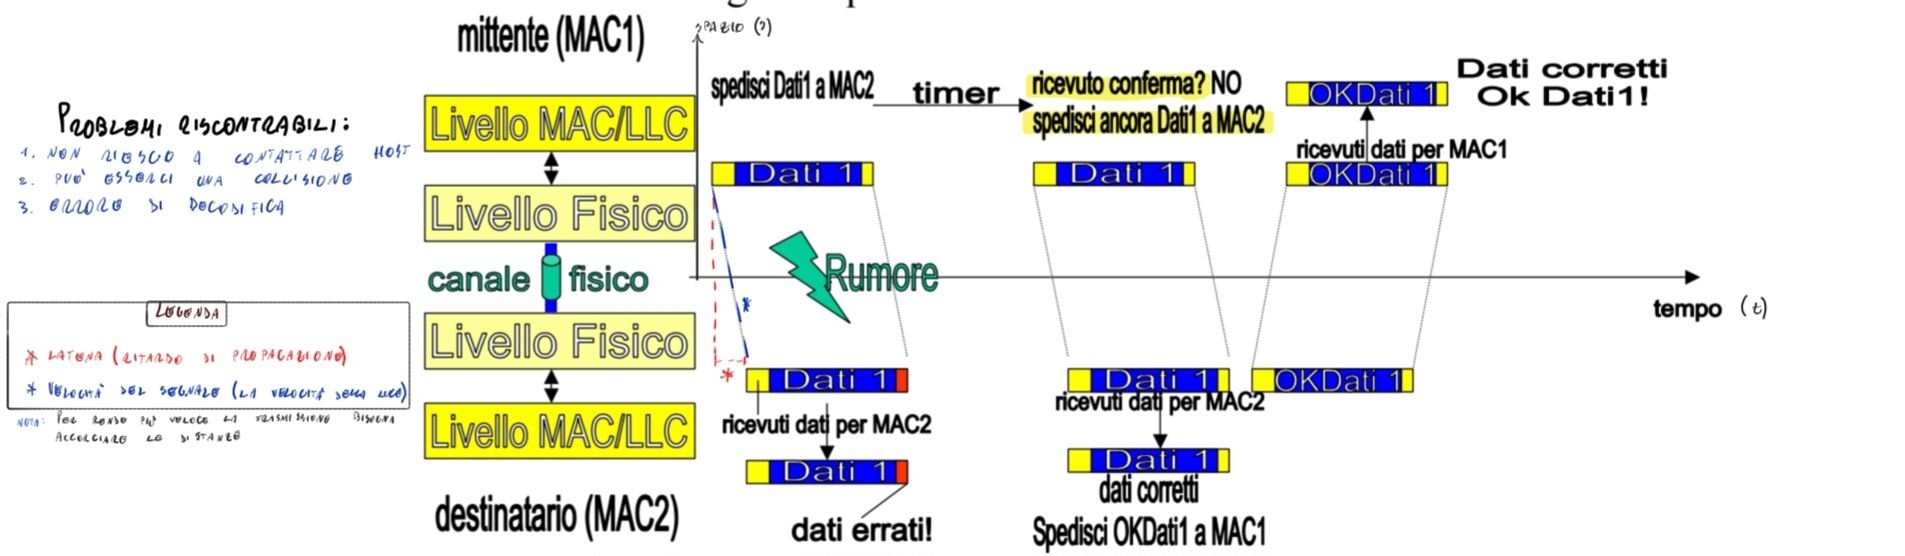
\includegraphics[width=1\linewidth]{foto reti di calcolatori/livello_LLC.jpg}
    \caption{Diagramma temporale di una trasmissione affidabile a livello LLC. L'immagine illustra la gestione di un errore fisico (rumore) tramite l'uso di un timer (timeout), la conseguente ritrasmissione e la ricezione finale del riscontro (ACK).}
    \label{fig:llc_ritrasmissione}
\end{figure}

\textbf{Dinamica della comunicazione temporale}
Il diagramma in Figura~\ref{fig:llc_ritrasmissione} mostra come il livello 2 (MAC/LLC) riesca a mascherare ai livelli superiori gli errori del mezzo trasmissivo, creando l'illusione di un canale affidabile. La linea del tempo scorre da sinistra a destra illustrando questi passaggi:

\begin{enumerate}[leftmargin=*]
    \item \textbf{Invio e attivazione del timer:} Il mittente (MAC1) spedisce il frame \texttt{Dati 1} sul canale fisico e, nello stesso istante, avvia un \textit{timer}. La linea tratteggiata orizzontale rossa rappresenta la \textbf{latenza} (ritardo di propagazione), che dipende dalla velocità fisica (linea tratteggiata bu diagonale) del segnale e dalla distanza tra gli host.
    \item \textbf{Interferenza e Dati errati:} Durante il tragitto, il segnale elettrico subisce un'interferenza a causa del \textbf{rumore}. Il destinatario (MAC2) riceve il frame ma, in fase di decodifica, i bit di controllo rivelano un errore. MAC2 scarta il pacchetto corrotto e resta in silenzio (non invia alcuna conferma).
    \item \textbf{Scadenza del Timeout e Ritrasmissione:} Il timer di MAC1 scade. Non avendo ricevuto alcun riscontro, il mittente deduce che c'è stato un problema e ritrasmette automaticamente una copia esatta di \texttt{Dati 1}, facendo ripartire il timer.
    \item \textbf{Ricezione corretta e ACK:} Questa volta il canale è pulito. MAC2 riceve e decodifica i dati correttamente, per poi inviare indietro un pacchetto di conferma chiamato \texttt{OKDati 1} (noto come \textit{Acknowledgment} o \textbf{ACK}).
    \item \textbf{Conclusione:} MAC1 riceve l'ACK prima che il timer scada. La comunicazione è conclusa con successo e i dati vengono passati ai livelli superiori.
\end{enumerate}

\begin{notebox}{\textbf{Problemi riscontrabili sul mezzo trasmissivo}}
Come annotato a lato dello schema, i principali problemi che il livello MAC/LLC si trova a dover gestire sul canale fisico includono:
\begin{itemize}
    \item Impossibilità fisica di contattare l'host destinatario (es. cavo scollegato o nodo offline).
    \item \textbf{Collisioni} dovute a trasmissioni simultanee sullo stesso mezzo condiviso.
    \item \textbf{Errori di decodifica} dei bit, causati da attenuazione o rumore elettromagnetico sul cavo (come nell'esempio appena visto).
\end{itemize}
\end{notebox}






\newpage
\subsection{Esempio completo di rete locale (LAN): tutti i dispositivi possono comunicare localmente tra di loro}

Diversi segmenti di rete locale possono essere collegati tramite bridge (B) o switch, hub (H) e repeater (R).  
La figura seguente mostra un esempio di rete locale composta da un segmento \textbf{Token Ring} (rosso) e da segmenti \textbf{Ethernet} (blu).

\begin{itemize}
    \item A sinistra, un calcolatore con scheda Token Ring e indirizzo MAC \textbf{A} è connesso all’anello Token Ring insieme ad altri tre calcolatori e un bridge (o switch) \textbf{B}, rappresentato in giallo per indicare l’azione a livello MAC/LLC.
    \item Il bridge \textbf{B} agisce da collegamento e da traduttore dei frame tra il segmento Token Ring (rosso) e i segmenti Ethernet (blu). Ha due connettori: uno Token Ring e uno Ethernet.
    \item Il segmento Ethernet del bridge \textbf{B} è connesso a un hub \textbf{H}, dal quale partono sei segmenti Ethernet punto-punto verso altri calcolatori (senza guardare contenuto di bit)
    \item Uno dei calcolatori è un repeater \textbf{R}, che propaga e amplifica i segnali verso un segmento Ethernet a bus con quattro calcolatori. Al termine del bus c’è un secondo repeater \textbf{R}, che estende la trasmissione verso l’ultimo segmento Ethernet a bus, collegato a un calcolatore con scheda Ethernet e indirizzo MAC \textbf{B}. 
    
    Se è soddisfatto dell'informazione crea ACK, inverte mittente e destinatario ed aspetta che sul canale si possa trasferire il frame con il percorso inverso
\end{itemize}

\textbf{Percorso logico di un frame (parte superiore immagine):}  
Un frame trasmesso dal calcolatore con MAC \textbf{A} al calcolatore con MAC \textbf{B} percorre tutti i segmenti e dispositivi intermedi:

\begin{itemize}
    \item Il frame sale al livello 2(MAC) solo nel bridge \textbf{B}, dove viene tradotto da Token Ring a Ethernet. Avviene il cosiddetto message passing e cambia la sintassi in funzione del protocollo di passaggio (a questo ci pensa il bridge)
    \item Nei repeater e hub, il frame viene semplicemente ricevuto e ritrasmesso al livello fisico (corrente elettrica che viaggia). Questi vengono aggiunti per non perdere il segnale che mano a mano diminuisce
    \item Se fosse necessario collegare più di due segmenti diversi, il bridge verrebbe sostituito da uno switch, che gestisce più interfacce e protocolli.
\end{itemize}

In questo modo è chiaro come sia possibile connettere diversi segmenti di rete locale e trasmettere frame tra due dispositivi qualsiasi, identificandoli tramite il loro indirizzo MAC.



\begin{figure}[H]
    \centering
    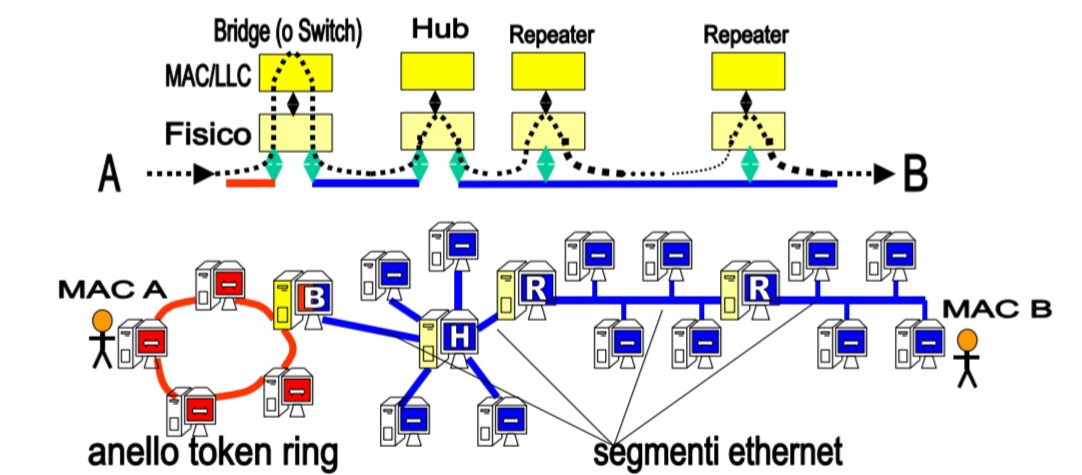
\includegraphics[width=0.7\linewidth]{foto reti di calcolatori/rete_locale.jpg}
    \caption{}
    \label{fig:placeholder}
\end{figure}


\subsection{Conclusioni}
Il livello MAC rappresenta un elemento fondamentale nelle reti locali, in quanto gestisce l’accesso al mezzo trasmissivo e il corretto incapsulamento dei dati provenienti dai livelli superiori.

La sua funzione principale è quella di garantire che più dispositivi possano condividere il canale di comunicazione in modo ordinato ed efficiente, evitando interferenze e collisioni e assicurando che ogni frame raggiunga correttamente il destinatario.

Durante la trasmissione, ogni frame viene arricchito con informazioni di controllo, come gli indirizzi MAC sorgente e destinazione e i campi di verifica degli errori, consentendo ai nodi della rete di riconoscere correttamente i destinatari e verificare l’integrità dei dati ricevuti.

Il meccanismo di accesso al canale varia a seconda della tecnologia: in reti cablate si possono verificare collisioni tra trasmissioni concorrenti, mentre in reti wireless o a topologia ad anello si adottano strategie diverse per ridurle o eliminarle. 

Inoltre, grazie a meccanismi di conferma e ritrasmissione, il livello MAC può garantire un’affidabilità locale rapida, limitata al collegamento tra due nodi adiacenti.

Quando più segmenti di rete sono interconnessi tramite dispositivi come bridge, hub o switch, il livello MAC si occupa di trasmettere i frame tra diverse topologie e tecnologie, consentendo la comunicazione tra dispositivi eterogenei e presentando ai livelli superiori un canale logico affidabile e privo di errori.

In sintesi, il livello MAC assicura un utilizzo efficiente del mezzo trasmissivo, l’integrità dei dati e la cooperazione tra dispositivi, costituendo la base operativa delle comunicazioni nelle reti locali moderne.


%===================== fine primo pacco di slide
\newpage


\section{Livello Rete (3)}

\subsection{Reti di reti e Internetworking}

Le reti locali non operano in modo isolato, ma sono connesse tra loro attraverso collegamenti organizzati in modo gerarchico.  
Ogni rete locale (LAN) dispone di un calcolatore speciale, detto \textbf{router}, che funge da rappresentante della rete e la collega ad altre reti tramite linee dati veloci o dorsali (\textbf{backbone}).


\begin{figure}[H]
    \centering
    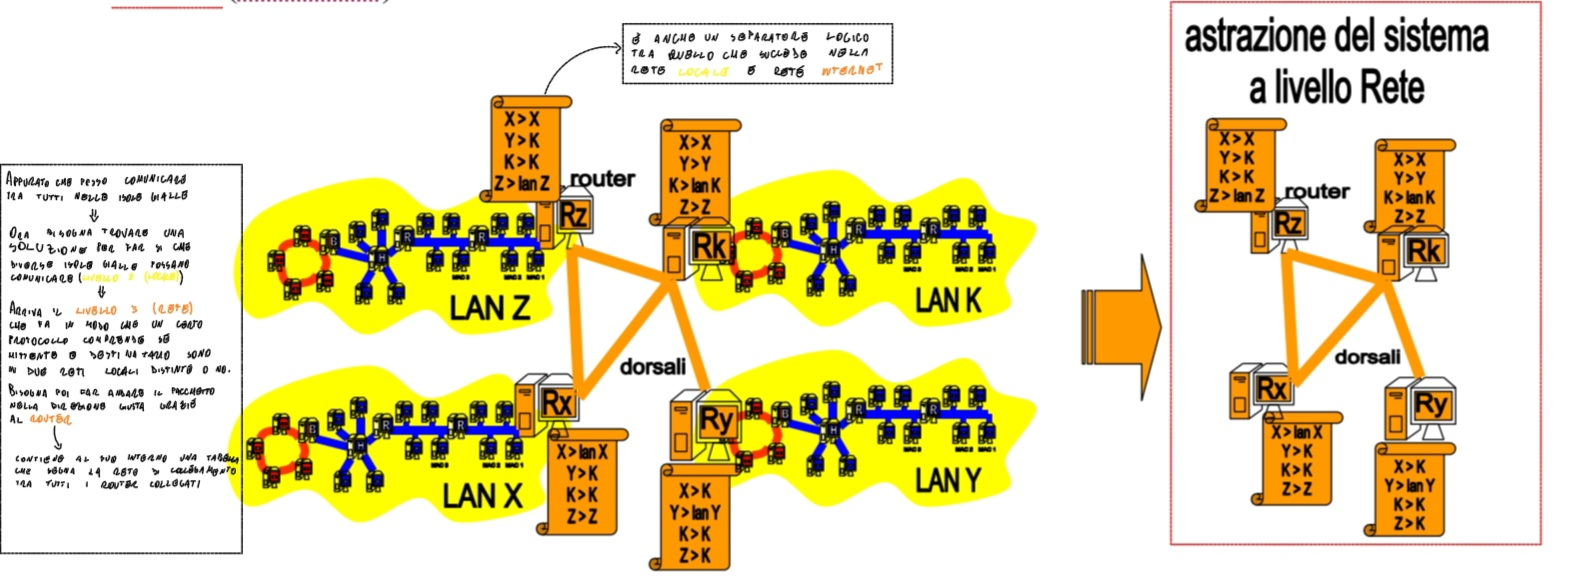
\includegraphics[width=1.1\linewidth]{foto reti di calcolatori/astrazione_rouer.jpg}
    \caption{Esempio di rete di reti locali e router collegati da dorsali, e l’astrazione dello stesso sistema al terzo livello (Rete) visto dai router.}
    \label{fig:placeholder}
\end{figure}

La figura rappresenta quattro reti locali, \textbf{X, Y, Z} e \textbf{K}, ciascuna dotata di un router (\textbf{R\textsubscript{x}}, \textbf{R\textsubscript{y}}, \textbf{R\textsubscript{z}}, \textbf{R\textsubscript{k}}).  
Ogni router è connesso alla propria rete locale e, tramite dorsali, anche ad altri router.  

Le dorsali e i router (in arancione) operano al \textbf{livello 3 (rete)} della gerarchia ISO/OSI.


Ogni router mantiene una \textbf{tabella di instradamento} che indica il primo router intermedio da utilizzare per raggiungere una determinata destinazione.  
Ad esempio, $R_z$ può comunicare con $R_y$ passando per il router intermedio $R_k$.  


Dal punto di vista del livello Rete, ogni router vede un’astrazione della rete complessiva, che nasconde i dettagli interni delle singole LAN, favorendo la \textbf{trasparenza dell’interconnessione} tra reti eterogenee.
\vspace{2cm}


\subsection{Gerarchia dei router default router e algotitmo funzionamento router }

La struttura dei router è tipicamente \textbf{gerarchica}.  
Ogni router può gestire più \textbf{sottoreti} interne, ciascuna con il proprio insieme di indirizzi IP.  

Tuttavia, non tutti i router sono direttamente connessi tra loro: 

quando un router non possiede una voce specifica nella sua tabella di instradamento per una certa destinazione, esso invia il pacchetto a un router di livello superiore detto \textbf{default router} (o \textbf{super router}).

\begin{itemize}
    \item Il default router rappresenta il punto di uscita predefinito per tutto il traffico destinato a reti non direttamente raggiungibili.
    \item In reti di grandi dimensioni, i default router formano una gerarchia: se due router di livello inferiore non possono comunicare direttamente, il traffico viene inoltrato a un router superiore, più specifico, che conosce il percorso appropriato.
\end{itemize}


\begin{figure}[H]
    \centering
    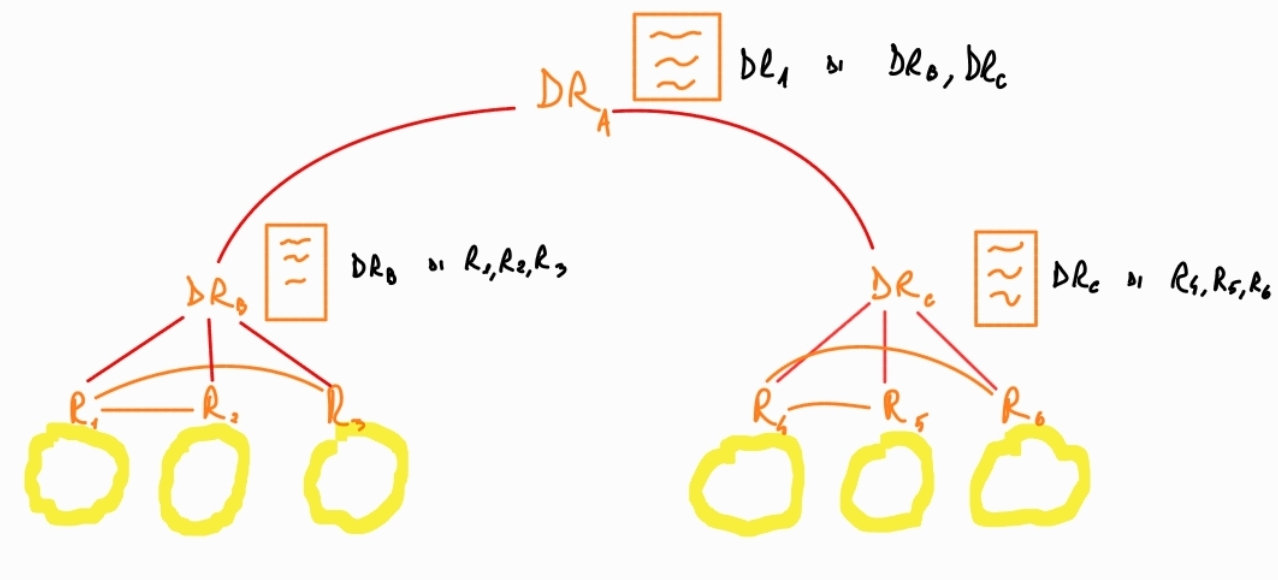
\includegraphics[width=1\linewidth]{foto reti di calcolatori/default_router.jpg}
    \caption{Collegamento gerarchico composto da default router per sottoreti specifiche}
    \label{fig:placeholder}
\end{figure}

\begin{algorithm}[H]
\SetAlgoLined
\caption{Algoritmo di un router}
\KwData{Pacchetto in arrivo da una delle interfacce di rete}
\KwResult{Pacchetto inoltrato verso la destinazione corretta}
\vspace{0.5 cm}

\While{il router è acceso}{
    Attendere l'arrivo di un pacchetto\;
    Leggere l'indirizzo IP di destinazione dal pacchetto\;
    
    \If{l'indirizzo di destinazione corrisponde a una rete locale}{
        Inoltrare il pacchetto all'host locale corrispondente\;
    }
    \Else{
        Cercare nella tabella di instradamento la rete di destinazione\;
        \If{voce trovata, il destinatario esite}{
            Inoltrare il pacchetto all'interfaccia di uscita indicata\;
        }
        \Else{
            Scartare il pacchetto e inviare un messaggio ICMP ``destinazione irraggiungibile'', quindi se ne dovrà occupare un default router\;
        }
    }
}
\end{algorithm}

\begin{notebox}{}
Il meccanismo del \textbf{default router} semplifica le tabelle di instradamento e riduce il numero di informazioni che ciascun router deve memorizzare, permettendo una gestione scalabile di reti complesse.
\end{notebox}

In questo modo, l’interconnessione di milioni di reti locali diventa possibile senza richiedere che ogni dispositivo conosca la topologia completa di Internet.  
La comunicazione tra due nodi qualsiasi avviene tramite una sequenza di router, ciascuno responsabile di un piccolo tratto del percorso complessivo.

\begin{defbox}{Router rappresentante}
Un \textbf{router rappresentante} per ogni rete locale è incaricato di:
\begin{itemize}
    \item ricevere i pacchetti destinati alla rete e recapitarli agli host interni;
    \item inoltrare i pacchetti in uscita verso i router delle reti di destinazione;
    \item comunicare con router di livello superiore (default router) quando non è in grado di determinare autonomamente il percorso.
\end{itemize}
\end{defbox}


\subsection{Internet Protocol (IP)}

Il concetto di rete si estende ora oltre la singola LAN, fino a una \textbf{rete di reti globali: Internet}.  

Il livello Rete di Internet è basato sul \textbf{protocollo IP (Internet Protocol)}, che definisce il formato dei pacchetti, le regole di indirizzamento e le procedure di instradamento.

\begin{itemize}
    \item \textbf{Nuovo tipo di Indirizzamento IP:} schema gerarchico,strutturato e globale che permette di identificare univocamente tutti i dispositivi di rete e allo stesso tempo la loro rete locale di appartenenza. Gli indirizzi usati permettono di identificare intere reti locali come un riferimento singolo nella gestione.
    \item \textbf{Instradamento (forwarding):} definisce il percorso dei pacchetti dal mittente al destinatario finale.
    
    È un \textbf{servizio connectionless}\footnote{\textit{Connectionless} significa "senza connessione": ogni pacchetto di dati viene inviato indipendentemente dagli altri, senza stabilire un collegamento continuo tra mittente e destinatario. Ciò implica che i pacchetti possono arrivare in ordine diverso o subire ritardi, come accade nel protocollo IP.}

    \item \textbf{Dispositivi di rete:} router con tabelle di instradamento che rappresentano la topologia della rete. 
    
    Tali router implementano i protocolli di aggiornamento delle tabelle di instradamento \textbf{(routing)}
    \item \textbf{Frammentazione \footnote{Vedi sezione 5.3.3 capitolo 5}:} suddivisione dei dati in pacchetti IP (fatta da IPv4  e non da IPv6).
    \item \textbf{Intestazione IP:} contiene gli indirizzi di mittente e destinatario a livello rete.
\end{itemize}

\begin{notebox}{}
Il livello Rete nasconde i dettagli interni delle LAN e fornisce un servizio di comunicazione tra reti eterogenee.
\end{notebox}

\subsection*{Instradamento-Routing \footnote{Vedi anche sezione 5.1.2 capitolo 5}}

\begin{notebox}{Instradamento e Routing}
\textbf{Instradamento} (\textit{forwarding}) è il processo con cui un dispositivo di rete, come un router, \textbf{decide a quale interfaccia inoltrare un pacchetto} in base alla sua destinazione.  
Il router consulta la \textbf{tabella di instradamento}, che associa le reti di destinazione alle interfacce o ai prossimi salti.


\textbf{Routing}, invece, è il processo più ampio di \textbf{determinare il percorso migliore} che i pacchetti devono seguire attraverso la rete (scrivendolo nella tabella di instradamento ), spesso calcolato da algoritmi di routing (come \textit{OSPF}, \textit{RIP}, \textit{BGP}).  
In sintesi:
\begin{itemize}
    \item \textbf{Routing} = scelta del percorso (decisione logica);
    \item \textbf{Instradamento} = inoltro del pacchetto lungo quel percorso (azione pratica).
\end{itemize}
\end{notebox}
\vspace{3cm}

\newpage
\subsection{Indirizzamento IPv4}

Il protocollo \textbf{IP} (\textit{Internet Protocol}) definisce una categoria di indirizzi chiamati \textbf{indirizzi IP}, utilizzati per identificare in modo univoco ogni dispositivo connesso a una rete che utilizza il protocollo TCP/IP.  

Ogni indirizzo IP è associato a una e una sola \textbf{interfaccia di rete} (scheda di rete)\footnote{Schede di rete differenti non possono condividere lo stesso indirizzo IP sulla stessa rete.}, creando un legame diretto con il suo indirizzo MAC.


\begin{defbox}{Indirizzo IPv4 e interfaccia}
Un \textbf{indirizzo IP} è un identificatore a \textbf{32 bit} (4 byte) associato
a un'\textbf{interfaccia} di un host o router -- non al dispositivo in sé.
Un'\textbf{interfaccia} è il punto di connessione fisico tra un dispositivo
e un link di rete.

Conseguenze pratiche importanti:
\begin{itemize}
    \item Un \textbf{router} ha tipicamente \emph{più} interfacce (una per
          ogni link a cui è connesso), ciascuna con il \emph{proprio}
          indirizzo IP distinto.
    \item Un \textbf{host} ha di solito una o due interfacce
          (es.\ Ethernet cablata + WiFi), ognuna con il proprio indirizzo.
    \item Cambiare scheda di rete significa cambiare interfaccia, non
          necessariamente indirizzo (che può essere riassegnato via DHCP).
\end{itemize}
\end{defbox}



\begin{itemize}
    \item \textbf{IPv4:} è la versione più diffusa del protocollo IP:
    \begin{itemize}
        \item \textbf{Formato \footnote{Per quanto riguarda il formato in questa sezione viene fatto vedere solo l'indirizzamento. per vedere il vero formato: IPv4 (cap 5 sezione 5.3.2) ; IPv6 (cap 5 sezione 5.3.7)}:} un indirizzo IPv4 è scritto in notazione \textbf{dotted-decimal} (\textit{decimale puntata}): i 32~bit vengono divisi in 4 gruppi da 8~bit (\textit{ottetti}), ciascuno convertito in decimale e separato da un punto. Ogni ottetto vale tra 0 e 255, quindi gli indirizzi IPv4 spaziano da \texttt{0.0.0.0} a \texttt{255.255.255.255}, per un totale di $2^{32} \approx 4.3$ miliardi di indirizzi distinti (esempio: \texttt{\textcolor{orange!85!black}{130.136}\textcolor{yellow!80!black}{.25.1}}).
        
        \[
        \underbrace{223}_{11011111}%
        \underbrace{.1}_{00000001}%
        \underbrace{.1}_{00000001}%
        \underbrace{.1}_{00000001}
        \;=\;
        \texttt{11011111\;00000001\;00000001\;00000001}
        \]

        \item \textbf{Struttura:} ogni indirizzo IP  si divide in due parti principali:
        \begin{itemize}
            \item \textbf{\textcolor{orange!85!black}{Network number}} – identifica una \textcolor{orange!85!black}{rete locale IP}(o la sottorete), cioè il \textbf{router} di una \textbf{“isola gialla”} di host collegati tramite lo stesso livello MAC.  
            Tutti i dispositivi che condividono lo stesso \textbf{network number} appartengono alla stessa isola gialla e possono comunicare direttamente senza passare da un router.
            
            \item \textbf{\textcolor{yellow!80!black}{Host number}} – identifica un singolo dispositivo (host) all’interno di quella rete gialla.  
        \end{itemize}
    \end{itemize}
\end{itemize}

\vspace{0.5cm} % Piccolo spazio per staccare la lista dal box

\begin{notebox}{L'indirizzo IP non identifica l'host, ma l'interfaccia}
Questo è un punto spesso frainteso. Se un laptop ha WiFi e Ethernet
attivi simultaneamente, ha \emph{due} indirizzi IP diversi. Analogamente,
un router con 4 porte ha 4 indirizzi IP. Quando si dice che
``il server ha indirizzo 192.168.1.10'' si intende che la sua interfaccia
di rete ha quell'indirizzo. La distinzione diventa critica quando si
configurano firewall, routing policy e NAT.
\end{notebox}

\begin{figure}[H]
    \centering
    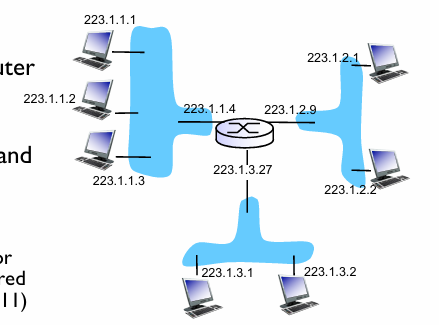
\includegraphics[width=0.82\textwidth]{foto reti di calcolatori/router_18.png}
    \caption{%
        \textbf{Indirizzi IP associati alle interfacce.}
        Nella figura si riconoscono tre \textit{cloud} di dispositivi
        connessi tra loro tramite un router centrale. Ogni interfaccia --
        sia degli host che del router -- porta il proprio indirizzo IP
        nella forma \texttt{223.1.x.y}. Il router centrale ha
        \textbf{tre interfacce} (indirizzi \texttt{223.1.1.4},
        \texttt{223.1.2.9}, \texttt{223.1.3.27}) perché è connesso a tre
        link distinti.
    }
    \label{fig:ip_intro}
\end{figure}


\begin{notebox}{}
    Due host possono avere lo stesso \textbf{host number} solo se appartengono a \textbf{isole arancioni differenti}.  
\end{notebox}

\subsubsection{Indirizzi IP Statici e Dinamici }
\begin{defbox}{Indirizzi IP statici e dinamici}
Quando un dispositivo si connette a Internet, riceve un indirizzo IP che può essere\footnote{Vedi anche sezione 3.3.12 per vedere come vengono assegnati}:
\begin{itemize}
    \item \textbf{IP statico}: l’associazione tra indirizzo MAC e indirizzo IP rimane costante nel tempo.  

    
    \textbf{Vantaggi:} utile per server, dispositivi di rete o servizi che devono essere sempre raggiungibili allo stesso indirizzo (es. server web, FTP, DNS).  

    
    \textbf{Svantaggi:} minore flessibilità e maggiore esposizione ad attacchi, poiché l’indirizzo resta invariato. 
    
    Inoltre se la macchina è spenta risulta essere irraggiungibile
    
    \item \textbf{IP dinamico}: l’associazione MAC–IP può cambiare a ogni connessione, tipicamente gestita da un server \textbf{DHCP} (\textit{Dynamic Host Configuration Protocol}).

    
    \textbf{Vantaggi:} maggiore sicurezza e utilizzo efficiente degli indirizzi IP.  

    
    \textbf{Svantaggi:} l’indirizzo può variare, rendendo difficile identificare in modo permanente un dispositivo.
\end{itemize}
\end{defbox}



\subsubsection*{Classi di indirizzi IPv4}

Gli indirizzi IPv4 sono storicamente suddivisi in tre classi principali, in base al numero di reti e host supportati. Per ciascuna classe si riportano il numero di bit e il numero di reti/host calcolato come potenza di 2:
\begin{figure}[H]
    \centering
    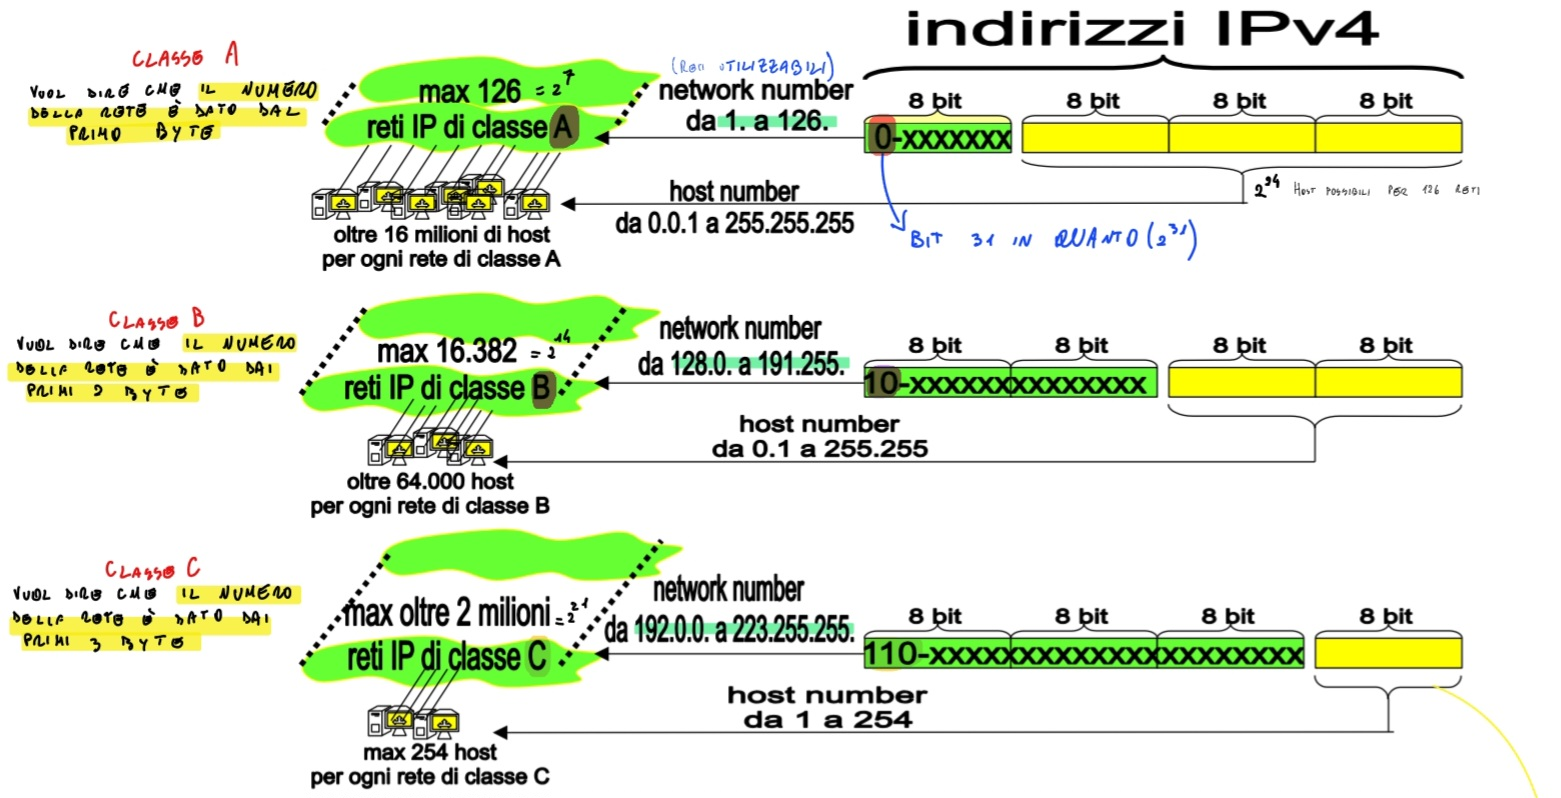
\includegraphics[width=1\linewidth]{foto reti di calcolatori/classi_IPv4.jpg}
    \label{fig:placeholder}
\end{figure}


\begin{itemize}
    \item \textbf{Classe A:}
    \begin{itemize}
        \item \textbf{\textcolor{orange!85!black}{Network number}}: 7 bit $\Rightarrow$ reti utilizzabili: $2^7 - 2 = 126$
        \item \textbf{\textcolor{yellow!80!black}{Host number}}: 24 bit $\Rightarrow$ host per rete: $2^{24} - 2 = 16.777.214$
        \item range indirizzi: \texttt{1.0.0.0 – 126.255.255.255}
    \end{itemize}

    \item \textbf{Classe B:}
    \begin{itemize}
        \item \textbf{\textcolor{orange!85!black}{Network number}}: 14 bit $\Rightarrow$ reti utilizzabili: $2^{14} - 2 = 16.382$
        \item \textbf{\textcolor{yellow!80!black}{Host number}}: 16 bit $\Rightarrow$ host per rete: $2^{16} - 2 = 65.534$
        \item range indirizzi: \texttt{128.0.0.0 – 191.255.255.255}
    \end{itemize}

    \item \textbf{Classe C:}
    \begin{itemize}
        \item \textbf{\textcolor{orange!85!black}{Network number}}: 21 bit $\Rightarrow$ reti utilizzabili: $2^{21} - 2 \approx 2.097.150$
        \item \textbf{\textcolor{yellow!80!black}{Host number}}: 8 bit $\Rightarrow$ host per rete: $2^8 - 2 = 254$
        \item range indirizzi: \texttt{192.0.0.0 – 223.255.255.255}
    \end{itemize}
\end{itemize}

\begin{notebox}{Perché si tolgono le combinazioni di tutti 0 e tutti 1}
Quando si calcola il numero di \textbf{reti} o di \textbf{host} in una classe IPv4, si usa la formula generale \(2^n - 2\), dove \(n\) è il numero di bit riservato alla parte \textbf{host number} (o, in passato, alla parte \textbf{network number}).  
Il motivo della sottrazione di 2 è il seguente:

\begin{itemize}
    \item La combinazione \textbf{tutti 0} (\(000\dots0\)) rappresenta l’\textbf{indirizzo di rete} (\textit{network address}).  
    Questo indirizzo identifica l’intera rete e non può essere assegnato a un singolo dispositivo (host).  
    \textit{Esempio:} per la rete \texttt{192.168.1.0/24}, l’indirizzo \texttt{192.168.1.0} è riservato come identificatore della rete.

    \item La combinazione \textbf{tutti 1} (\(111\dots1\)) rappresenta l’\textbf{indirizzo di broadcast}.  
    Questo indirizzo serve per inviare un pacchetto a \textbf{tutti} gli host della stessa rete.  
    \textit{Esempio:} nella rete \texttt{192.168.1.0/24}, l’indirizzo \texttt{192.168.1.255} è quello di broadcast.
\end{itemize}

Di conseguenza, questi due indirizzi non possono essere assegnati a nessun host, e vengono sottratti dal conteggio totale delle combinazioni possibili.  
Ecco perché il numero effettivo di host in una rete è \(2^n - 2\).
\end{notebox}


\begin{esempiobox}{Esempi di classi IPv4}

\textbf{Classe A:} indirizzo IP \texttt{10.23.45.67}  
\begin{itemize}[leftmargin=*]
    \item Decimale: 10.23.45.67
    \item Binario: \textcolor{orange!85!black}{\textbf{0}0001010}.\textcolor{yellow!80!black}{00010111.00101101.01000011}  
    \item Analisi: primo byte $\rightarrow$ \textcolor{orange!85!black}{network number (7 bit) = 10}, 
    
    restanti 3 byte $\rightarrow$ \textcolor{yellow!80!black}{host number (24 bit) = 23.45.67}
\end{itemize}

\textbf{Classe B:} indirizzo IP \texttt{172.16.45.67}  
\begin{itemize}[leftmargin=*]
    \item Decimale: 172.16.45.67
    \item Binario: \textcolor{orange!85!black}{\textbf{10}101100.00010000}.\textcolor{yellow!80!black}{00101101.01000011}  
    \item Analisi: primi 2 byte $\rightarrow$ \textcolor{orange!85!black}{network number (14 bit) = 172.16}, 
    
    ultimi 2 byte $\rightarrow$ \textcolor{yellow!80!black}{host number (16 bit) = 45.67}
\end{itemize}

\textbf{Classe C:} indirizzo IP \texttt{192.168.45.67}  
\begin{itemize}[leftmargin=*]
    \item Decimale: 192.168.45.67
    \item Binario: \textcolor{orange!85!black}{\textbf{110}00000.10101000.00101101}.\textcolor{yellow!80!black}{01000011}  
    \item Analisi: primi 3 byte $\rightarrow$ \textcolor{orange!85!black}{network number (21 bit) = 192.168.45}, 
    
    ultimo byte $\rightarrow$ \textcolor{yellow!80!black}{host number (8 bit) = 67}
\end{itemize}

\end{esempiobox}


\newpage
\subsection{Sottoreti (subnetwork)}

Le \textbf{sottoreti} (\textit{subnetwork}) rappresentano un'estensione del concetto di rete IP, che consente di suddividere una rete più grande in più reti logiche più piccole e gestibili, dette appunto sottoreti.  

Questo approccio migliora l'organizzazione gerarchica, l'efficienza dell'instradamento e la sicurezza.

\begin{defbox}{Subnet}
Una \textbf{subnet} (sottorete) è un insieme di interfacce di dispositivi
che:
\begin{enumerate}
    \item Condividono la stessa \textbf{parte di rete} (\textit{network
          part}) dell'indirizzo IP -- i bit più significativi.
    \item Possono comunicare direttamente tra loro \textbf{senza passare
          per un router} -- sono sullo stesso segmento fisico di rete.
\end{enumerate}

\textbf{Procedura per identificare le subnet}: si ``staccano'' mentalmente
tutte le interfacce dai loro host e router. Ogni isola di rete isolata
risultante è esattamente una subnet.
\end{defbox}
\subsubsection{ESEMPIO 1}

\begin{figure}[H]
    \centering
    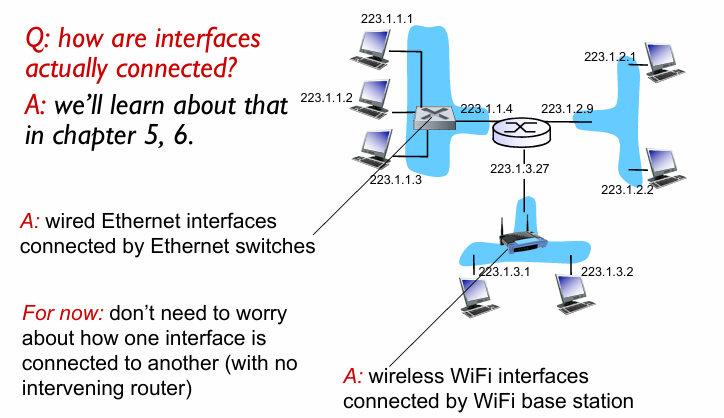
\includegraphics[width=0.8\textwidth]{router_19.png}
    \caption{%
        \textbf{Rete composta da 3 subnet con maschera \texttt{/24}.}
        Applicando la procedura di identificazione -- staccare ogni
        interfaccia dal suo dispositivo -- emergono tre isole isolate,
        ciascuna una subnet distinta:
        \textbf{subnet \texttt{223.1.1.0/24}}: contiene gli host
        \texttt{223.1.1.1}, \texttt{.2}, \texttt{.3} e l'interfaccia
        \texttt{223.1.1.4} del router;
        \textbf{subnet \texttt{223.1.2.0/24}}: contiene \texttt{223.1.2.1},
        \texttt{.2} e l'interfaccia \texttt{223.1.2.9} del router;
        \textbf{subnet \texttt{223.1.3.0/24}}: contiene \texttt{223.1.3.1},
        \texttt{.2}, \texttt{.27} e l'interfaccia del router.
        Tutte e tre condividono i primi 24~bit del prefisso
        (\texttt{223.1.x}) e differiscono solo nel terzo ottetto.
        La maschera \texttt{/24} si chiama \textbf{subnet mask}.%
    }
    \label{fig:subnets_3}
\end{figure}
\newpage
\subsubsection{ESEMPIO 2}

\begin{figure}[H]
    \centering
    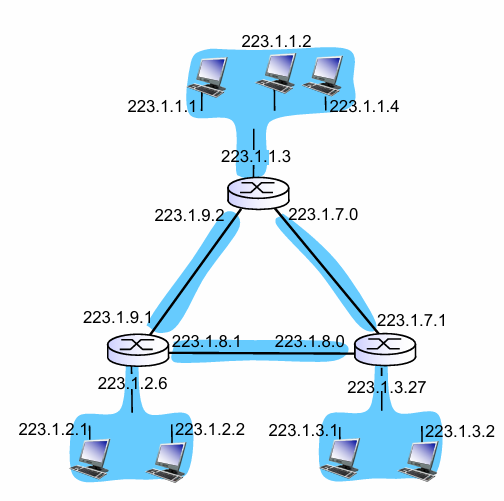
\includegraphics[width=0.8\textwidth]{router_20.png}
    \caption{%
        \textbf{Rete complessa: contare le subnet.}
        Per determinare il numero esatto di sottoreti, bisogna isolare logicamente ogni interfaccia dei router. In questa topologia ci sono \textbf{6 subnet} in totale, divise in due categorie. 
        \textbf{Tre subnet locali (LAN)} che collegano gli host ai rispettivi router: la \texttt{223.1.1.0/24} (in alto), la \texttt{223.1.2.0/24} (in basso a sinistra) e la \texttt{223.1.3.0/24} (in basso a destra).
        \textbf{Tre subnet punto-punto} che collegano esclusivamente le interfacce dei router tra loro: la \texttt{223.1.8.0/24} (che unisce i due router in basso), la \texttt{223.1.7.0/24} (tra il router in alto  e quello in basso a destra) e la \texttt{223.1.9.0/24} (tra il router in alto  e quello in basso a sinistra).
    }
    \label{fig:router_6_subnet}
\end{figure}

\begin{notebox}{Anomalia nella figura -- indirizzo di rete
assegnato a un'interfaccia router}

Nella figura {3.17} si nota una situazione
apparentemente scorretta: le interfacce dei router sui link
punto-punto ricevono indirizzi come \texttt{223.1.7.0} e
\texttt{223.1.8.0}, dove l'ultimo ottetto è \textbf{zero}.

Per convenzione, l'indirizzo con tutti i bit host a 0 è
l'\textbf{indirizzo di rete} (network address) e
\textbf{non dovrebbe essere assegnato ad alcun dispositivo}:
\begin{itemize}
    \item \texttt{223.1.8.\textbf{0}} $\Rightarrow$ dovrebbe
          essere l'identificativo della subnet
          \texttt{223.1.8.0/24}, non l'indirizzo
          dell'interfaccia di un router.
    \item \texttt{223.1.7.\textbf{0}} $\Rightarrow$ stessa
          anomalia.
\end{itemize}

Nella realtà, queste interfacce andrebbero configurate con
indirizzi host validi, ad esempio \texttt{223.1.8.\textbf{1}}
e \texttt{223.1.8.\textbf{2}} per i due capi del link
punto-punto (oppure usare un blocco \texttt{/30} che lascia
solo 2 indirizzi host disponibili, evitando lo spreco di 254
indirizzi per un link con soli 2 dispositivi):

\begin{center}
\begin{tabular}{lll}
\toprule
\textbf{Cosa} & \textbf{Figura (errato)} &
\textbf{Configurazione corretta} \\
\midrule
Subnet del link    & \texttt{223.1.8.0/24}
                   & \texttt{223.1.8.0/30} \\
Router destro    & \texttt{223.1.8.0} (!)
                   & \texttt{223.1.8.1} \\
Router sinistro      & \texttt{223.1.8.1}
                   & \texttt{223.1.8.2} \\
Indirizzo di rete  & (usato come host!)
                   & \texttt{223.1.8.0} (riservato) \\
Broadcast          & \texttt{223.1.8.255}
                   & \texttt{223.1.8.3} (riservato) \\
\bottomrule
\end{tabular}
\end{center}

La figura delle slide usa questi indirizzi
\textbf{a scopo didattico} per semplificare la lettura
visiva della topologia -- nella pratica un amministratore
di rete non assegnerebbe mai \texttt{.0} a un'interfaccia
perché causerebbe ambiguità: non sarebbe chiaro se
\texttt{223.1.8.0} si riferisce alla subnet o all'host.
\end{notebox}



\begin{esempiobox}{Come leggere la subnet mask -- e casi pratici}

La notazione \texttt{223.1.1.0/24} si legge: ``rete
\texttt{223.1.1.0} con maschera a 24~bit''.
\begin{itemize}
    \item I \textbf{primi 24~bit} (\texttt{223.1.1}) identificano
          la subnet.
    \item Gli \textbf{ultimi 8~bit} identificano l'host: da
          \texttt{.0} (indirizzo di rete, non assegnabile) a
          \texttt{.255} (broadcast, non assegnabile) $\Rightarrow$
          \textbf{254 host utilizzabili}.
    \item Forma dotted-decimal: \texttt{255.255.255.0}.
\end{itemize}

In generale: una maschera \texttt{/x} permette $2^{32-x}$
indirizzi, di cui $2^{32-x}-2$ assegnabili agli host.

\vspace{0.4em}
\textbf{Fino a quale maschera posso spingermi?}

Per la subnet in alto nella figura {5.24} (es.\
\texttt{223.1.1.0}), la maschera più lunga tecnicamente
utilizzabile è \texttt{/29}:
\begin{center}
\begin{tabular}{lccc}
\toprule
\textbf{Maschera} & \textbf{Indirizzi totali} &
\textbf{Host usabili} & \textbf{Note} \\
\midrule
/24 & 256 & 254 & Caso della figura \\
/28 & 16  & 14  & Piccola \\
/29 & 8   & 6   & Minimo pratico con più host \\
/30 & 4   & 2   & Solo link punto-punto \\
/31 & 2   & 2   & Solo P2P (RFC 3021) \\
/32 & 1   & 0   & Indirizzo singolo (loopback) \\
\bottomrule
\end{tabular}
\end{center}
Non ha senso scendere oltre \texttt{/29} per una subnet con più
host: con \texttt{/30} si hanno solo 2 indirizzi utili (adatti
esclusivamente a link punto-punto tra due router), e con
\texttt{/31} o \texttt{/32} non ci sono host utili nel senso
tradizionale.

\end{esempiobox}
\newpage

\subsubsection{ESEMPIO 3}
La figura \ref{fig:sottoreti} mostra, a sinistra, uno schema gerarchico di una rete di \textbf{classe B}.  
In cima si trova il \textbf{router principale} (\textbf{default router}) della rete \texttt{130.136}, con indirizzo IP \textcolor{orange!85!black}{130.136.0.254}.  
Alla rete \texttt{130.136} appartengono tre router subordinati, con indirizzi IP:
\begin{itemize}
    \item \textcolor{orange!85!black}{130.136.1.254} (amministratore della sottorete \texttt{130.136.1.})
    \item \textcolor{orange!85!black}{130.136.2.254} (amministratore della sottorete \texttt{130.136.2.})
    \item \textcolor{orange!85!black}{130.136.3.254} (amministratore della sottorete \texttt{130.136.3.})
\end{itemize}

\begin{notebox}{}
Quando una rete o sottorete viene \textbf{collegata a Internet}, ogni router subordinato gestisce una porzione specifica della rete principale e deve conoscere i seguenti parametri fondamentali:

\begin{enumerate}
    \item La propria \textbf{maschera di rete} (\textcolor{green!85!black}{netmask}), che definisce quanti bit identificano la parte di rete e quanti quella degli host.
    \item L’indirizzo IP della \textbf{rete e sottorete di competenza}, calcolato tramite operazione logica AND bit a bit tra IP e netmask\footnote{vedi esempio a pag 40}.
    \item L’indirizzo del \textbf{default router} superiore (gateway predefinito), necessario per instradare i pacchetti verso reti esterne o Internet.
\end{enumerate}

In questo modo, ogni router locale può gestire correttamente il traffico interno alla propria sottorete e inoltrare i pacchetti destinati ad altre reti al router di livello superiore.
\end{notebox}


\begin{figure}[H]
    \centering
    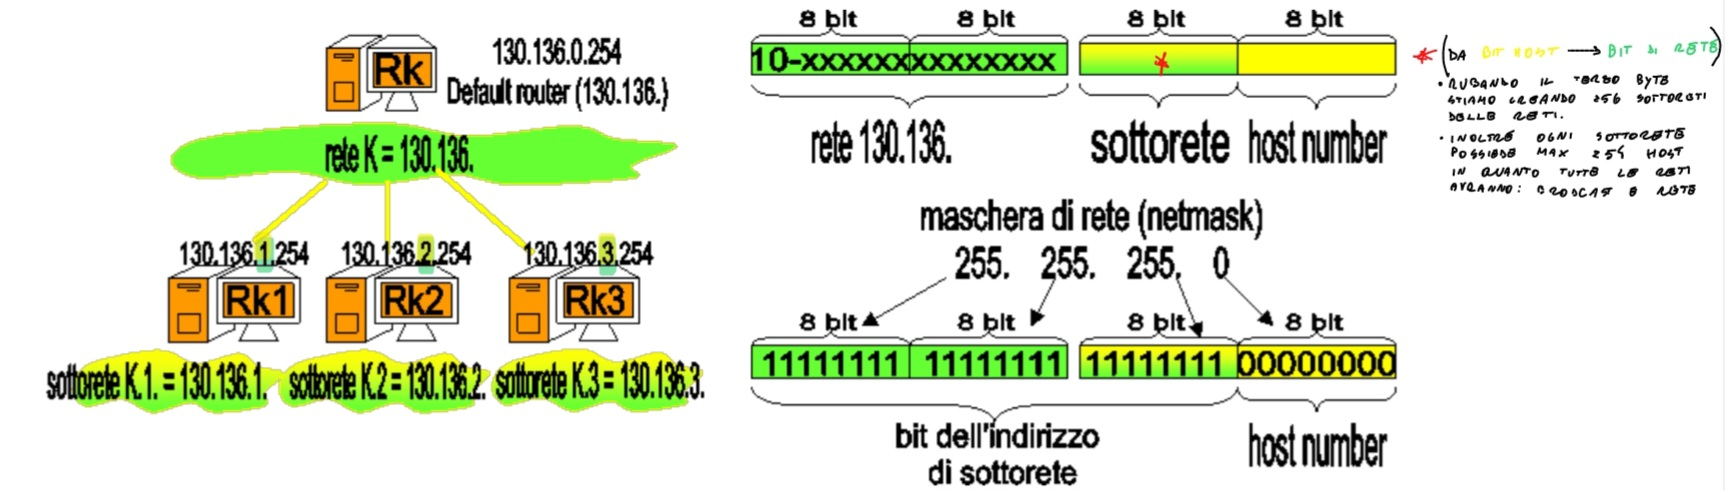
\includegraphics[width=1\linewidth]{foto reti di calcolatori/subnetwork.jpg}
    \caption{Esempio di rete IP di classe B suddivisa in sottoreti.}
    \label{fig:sottoreti}
\end{figure}

La \textbf{maschera di rete (netmask)} è uno strumento fondamentale per distinguere le due parti logiche di un indirizzo IP:
\begin{itemize}
    \item \textcolor{green!85!black}{Indirizzo di sottorete (subnetwork address):} corrisponde ai bit in cui la netmask ha valore \textbf{1}, partendo da sinistra, servono  a definire quali bit degli indirizzi IP vadano interpretati come numero della sottorete
    \item \textcolor{yellow!85!black}{Host number:} corrisponde ai bit in cui la netmask ha valore \textbf{0}, e servono a descrivere quali bit vanno considerati come il numero dell' host appartenente a quella sottorete.
\end{itemize}

Nell’esempio mostrato, i primi 24 bit (3 byte) della netmask sono tutti impostati a uno:
\[
\texttt{255.255.255.0} = \textcolor{green!85!black}{11111111.11111111.11111111.}\textcolor{yellow!85!black}{00000000}
\]
Questo significa che i primi tre byte dell’indirizzo IP rappresentano il numero della sottorete, mentre l’ultimo byte rappresenta il numero dell’host.

\begin{esempiobox}{Esempio pratico}
Data la rete di classe B \texttt{130.136.0.0/16}, decidiamo di creare 256 sottoreti utilizzando la netmask \texttt{255.255.255.0}.

\begin{itemize}
    \item \texttt{130.136.1.0} → rete: 130.136; sottorete: 1  
    \item \texttt{130.136.2.0} → rete: 130.136; sottorete: 2  
    \item \texttt{130.136.1.22} → host 22 della sottorete 1  
    \item \texttt{130.136.3.48} → host 48 della sottorete 3  
\end{itemize}

Ogni sottorete è amministrata da un router dedicato e si collega al default router di rete \texttt{130.136.0.254}.
\end{esempiobox}


\begin{notebox}{Perché il router ha per convenzione l’ultimo indirizzo della sottorete}
Per convenzione, si assegna spesso al \textbf{router} di una sottorete l’\textbf{ultimo indirizzo disponibile} della rete (es. \texttt{.254} in una rete /24).  
Questa pratica non è obbligatoria, ma è adottata per motivi di:
\begin{itemize}
    \item \textbf{Uniformità e riconoscibilità:} sapere che il router di ogni sottorete termina con .254 rende la configurazione e la manutenzione più intuitive;
    \item \textbf{Chiarezza amministrativa:} facilita la documentazione e la gestione centralizzata degli indirizzi IP;
    \item \textbf{Separazione logica:} il primo indirizzo (\texttt{.1}) è solitamente assegnato a un server o gateway locale, mentre l’ultimo (\texttt{.254}) identifica il router che instrada il traffico esterno.
\end{itemize}
In altre parole, assegnare il router all’ultimo host segue una convenzione pratica per rendere la rete più leggibile e standardizzata.
\end{notebox}

\begin{esempiobox}{ Verifica se un indirizzo è una maschera di rete}
Vogliamo verificare se i seguenti indirizzi sono \textbf{maschere di rete} valide.

\[
\begin{array}{ll}
1) & \texttt{254.0.0.0} \Rightarrow 11111110.00000000.00000000.00000000 \\
2) & \texttt{224.0.0.0} \Rightarrow 11100000.00000000.00000000.00000000 \\
3) & \texttt{255.248.0.0} \Rightarrow 11111111.11111000.00000000.00000000 \\
4) & \texttt{254.255.0.0} \Rightarrow 11111110.11111111.00000000.00000000 \\
5) & \texttt{255.255.248.128} \Rightarrow 11111111.11111111.11111000.10000000 \\
\end{array}
\]

\begin{itemize}
    \item Le maschere \texttt{254.0.0.0}, \texttt{224.0.0.0} e \texttt{255.248.0.0} sono valide, perché i bit a \textbf{1} sono tutti contigui da sinistra.
    \item Le maschere \texttt{254.255.0.0} e \texttt{255.255.248.128} non sono valide: i bit a 1 e a 0 si alternano, violando la regola di contiguità.
\end{itemize}

\begin{notebox}{Regola fondamentale}
Una \textbf{maschera di rete} è valida se e solo se i bit a \textbf{1} sono tutti contigui a partire da sinistra e seguiti solo da bit a \textbf{0}.
\end{notebox}
\end{esempiobox}


\begin{esempiobox}{Utilizzo sensato indirizzi IP tramite netmask }
    Vogliamo ora fare in modo che gli indirizzi IP siano:
    \begin{itemize}
        \item Utilizzati al minimo
        \item consumati al meglio
        
    \end{itemize}
    Questi due fattori li dimostreremo tramite un esempio

    \begin{figure}[H]
        \centering
        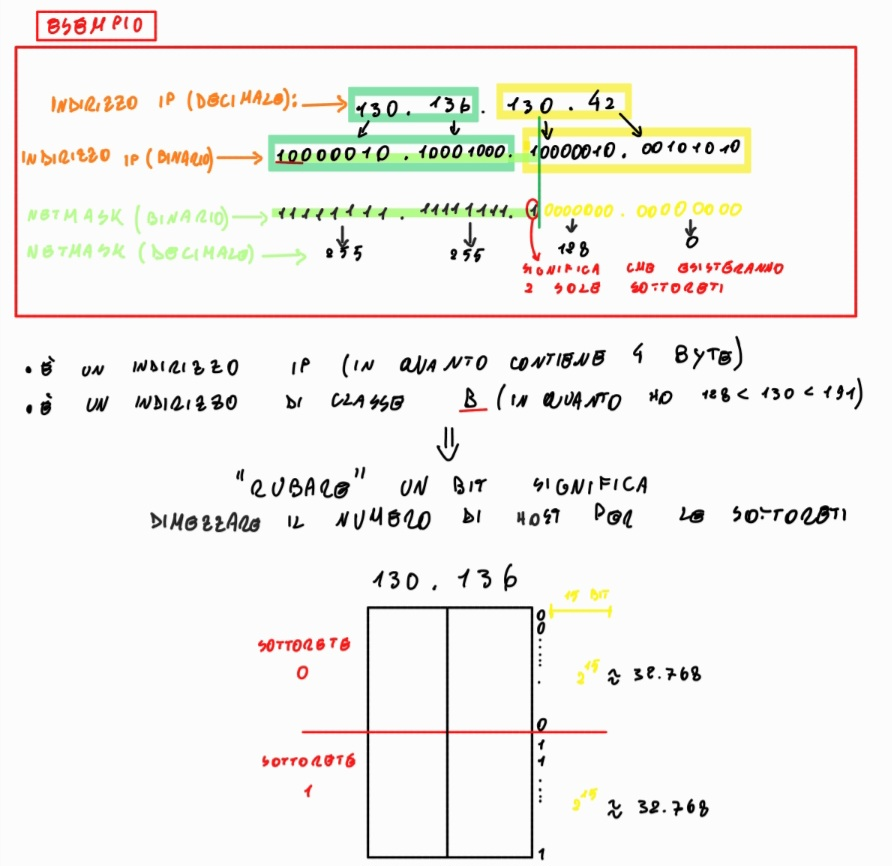
\includegraphics[width=0.7\linewidth]{foto reti di calcolatori/es_ip(1).jpg}
        \label{fig:placeholder}
    \end{figure}

    Proseguiamo mostrando com'è stato calcolato l'indirizzo IP inerente alla rete e sottorete considerata:

    \begin{figure}[H]
        \centering
        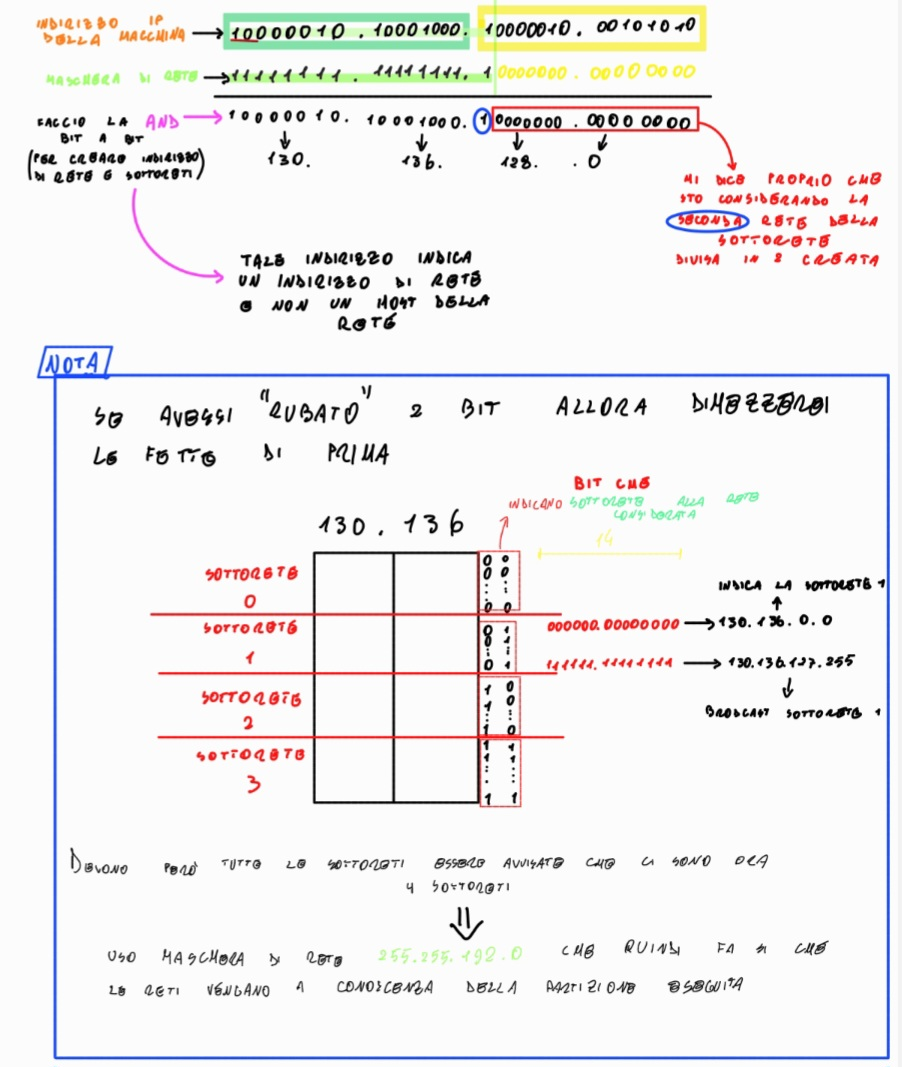
\includegraphics[width=0.7\linewidth]{foto reti di calcolatori/es_ip(2).jpg}
        \label{fig:placeholder}
    \end{figure}
\end{esempiobox}
    

\newpage
\subsection{CIDR}

\begin{defbox}{CIDR}
\textbf{CIDR} (\textit{Classless InterDomain Routing}) è lo schema di
indirizzamento adottato in cui la \textbf{lunghezza del prefisso
di rete è arbitraria}: non deve essere necessariamente 8, 16 o 24~bit
come nelle classi A, B, C dello schema classful precedente.

Notazione standard: \quad \texttt{a.b.c.d/x}

dove \textbf{x} è il numero di bit della parte di rete
(\textit{prefix length}).
\end{defbox}
\begin{notebox}{Notazione CIDR (/n)}
La notazione \textbf{CIDR} specifica, dopo una barra obliqua, il \textbf{numero di bit riservati alla parte di rete (network + sottorete)} di un indirizzo IPv4.

\[
\texttt{130.136.0.0/16}
\]

indica che i primi \textbf{16 bit} dell’indirizzo appartengono alla parte di \textbf{rete}, mentre i restanti \textbf{16 bit} rappresentano la parte di \textbf{host}.  
In binario:

\[
\underbrace{\colorbox{green!40}{11111111.11111111}}_{\text{16 bit di rete}}
\underbrace{\colorbox{yellow!40}{00000000.00000000}}_{\text{16 bit di host}}
\]

In forma decimale, la \textbf{maschera di rete (subnet mask)} corrispondente è:

\[
255.255.0.0
\]

\textbf{Vantaggi: \textbf{lunghezza del prefisso
di rete è arbitraria}}

la notazione CIDR è più compatta e flessibile delle vecchie classi A, B e C, poiché permette di definire reti di qualsiasi dimensione senza dover rispettare rigidamente le classi standard.  
Ad esempio:
\[
\texttt{/24} = 255.255.255.0, \quad \texttt{/20} = 255.255.240.0, \quad \texttt{/28} = 255.255.255.240
\]


\end{notebox}

\begin{notebox}{Perché CIDR ha sostituito il classful addressing}
Nel sistema classful originale esistevano solo tre taglie di rete:
\begin{itemize}
    \item \textbf{Classe A} (\texttt{/8}): $2^{24} \approx 16$ milioni
          di host -- enorme, assegnata a poche organizzazioni
          (IBM, MIT, \ldots).
    \item \textbf{Classe B} (\texttt{/16}): $2^{16} \approx 65$K host
          -- spesso troppo grande per un'azienda media.
    \item \textbf{Classe C} (\texttt{/24}): 254 host -- spesso troppo
          piccola.
\end{itemize}
Il risultato era uno \textbf{spreco enorme} di indirizzi: un'azienda con
300 dipendenti prendeva una classe~B (65K indirizzi) lasciandone
inutilizzati 64K. CIDR risolve questo con la granularità arbitraria:
la stessa azienda riceve una \texttt{/23} (510 indirizzi), spreco minimo.

\end{notebox}


\newpage
\subsection{Instradamento (forwarding) dei pacchetti}

L'\textbf{instradamento} (\textit{forwarding}) dei pacchetti è il processo mediante il quale un router decide dove inviare un pacchetto IP in base all'indirizzo di destinazione.  
In una rete gerarchica, l'instradamento avviene spesso in più passaggi, passando dai router locali ai router di livello superiore fino a raggiungere la sottorete del destinatario.
\begin{figure}[H]
    \centering
    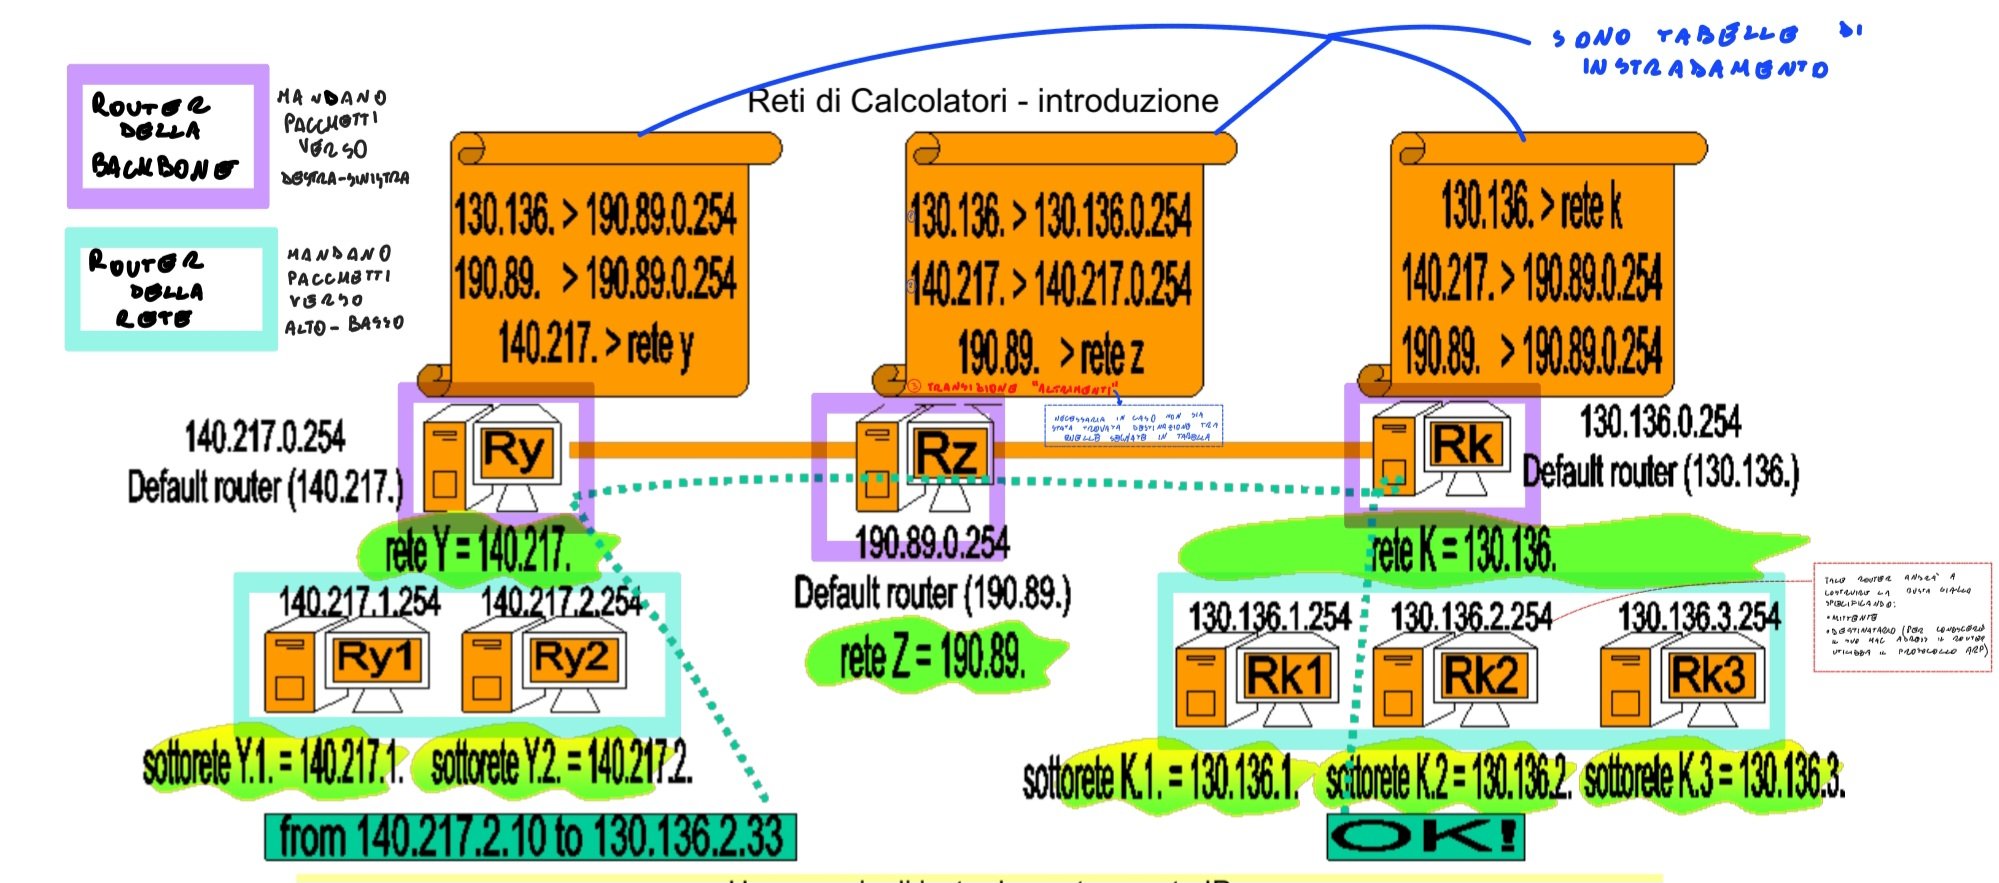
\includegraphics[width=1\linewidth]{foto reti di calcolatori/forwarding.jpg}
    \label{fig:placeholder}
\end{figure}

\begin{esempiobox}{Esempio pratico di instradamento IP}
Consideriamo il seguente scenario:

\begin{itemize}
    \item Host mittente: \texttt{140.217.2.10}  
    \item Host destinatario: \texttt{130.136.2.33}  
\end{itemize}

Il pacchetto IP segue il seguente percorso:

\begin{enumerate}
    \item Il pacchetto viene inviato dall'host \texttt{140.217.2.10} al router della sottorete \texttt{140.217.2.254}.
    \item Il router nota che il destinatario non appartiene alla sottorete e lo inoltra al router di livello superiore: \texttt{140.217.0.254}.
    \item Il router \texttt{140.217.0.254} consulta la propria tabella di forwarding e scopre che il pacchetto deve essere inoltrato al router intermedio \texttt{190.89.0.254}.
    \item Il router intermedio \texttt{190.89.0.254} verifica la tabella di forwarding e inoltra il pacchetto al router \texttt{130.136.0.254}.
    \item Il router \texttt{130.136.0.254} identifica che il pacchetto appartiene alla propria rete (\texttt{130.136.-.-}) e lo inoltra alla sottorete corretta.
    \item Il router di sottorete \texttt{130.136.2.254} inoltra il pacchetto all'host destinatario \texttt{130.136.2.33}.
\end{enumerate}

Alla fine del percorso, il pacchetto arriva correttamente al destinatario.  
Questo esempio mostra come, anche in reti con molti host e sottoreti, l'instradamento rimanga semplice e gerarchico. Le tabelle di forwarding contengono solo informazioni necessarie al livello locale, evitando la gestione di tutte le sottoreti dell'intera rete.
\end{esempiobox}



\begin{notebox}{Aspetti importanti dell'instradamento gerarchico}
\begin{itemize}
    \item L'instradamento è \textbf{gerarchico}: ogni router gestisce solo il proprio livello di rete o sottorete.
    \item Le tabelle di forwarding sono \textbf{semplici e compatte}, contenendo solo informazioni rilevanti per il router.
    \item Anche con un numero elevato di host e sottoreti, il processo di instradamento rimane costituito da operazioni di base semplici e rapide.
\end{itemize}
\end{notebox}


\subsection{Il problema del routing}

Il \textbf{routing} è il protocollo attraverso il quale i router mantengono aggiornate le proprie
\textbf{tabelle di forwarding}, garantendo che i pacchetti IP possano attraversare la rete
seguendo percorsi validi ed efficienti.

Il problema principale è che i \textbf{cammini di rete possono cambiare} nel tempo, causando
l’invalidazione delle tabelle presenti nei router.

\begin{itemize}
    \item In reti \textbf{senza fili}, la mobilità degli host può modificare dinamicamente la topologia.
    \item Guasti a linee, collegamenti o router possono rendere irraggiungibili intere sottoreti.
    \item Cambiamenti negli \textbf{accordi di servizio tra  Sistemi Autonomi (AS)} \footnote{\textbf{} grandi porzioni di Internet costituite da una o più reti gestite da un'unica organizzazione (operatore, università, azienda, ISP).  
Ogni AS applica una propria politica di routing e comunica con gli altri AS tramite protocolli come BGP. Gli AS si comportano come “domini amministrativi” indipendenti che decidono quali cammini consentire o negare ai pacchetti. Tutti i router di una stessa AS seguono le stesse regole di gestione}
possono cambiare i percorsi ammessi.
\end{itemize}

Quando ciò accade, alcuni router possono avere tabelle di instradamento \textbf{obsolete}:
\begin{itemize}
    \item pacchetti smarriti; 
    \item pacchetti che seguono cammini alternativi e arrivano in ordine errato;
    \item rallentamenti o congestioni non previste.
\end{itemize}

\begin{notebox}{Reazione dei router}
I router devono reagire prontamente ai cambiamenti della topologia, aggiornando le loro tabelle.
Per farlo utilizzano \textbf{protocolli (algoritmi) di routing} che permettono di:
\begin{itemize}
    \item inviare richieste per scoprire nuovi cammini disponibili;
    \item aggiornare le tabelle di forwarding con il percorso migliore.
\end{itemize}
\end{notebox}

Esempi di protocolli di routing utilizzati su Internet:
\begin{itemize}
    \item \textbf{RIP} (Routing Information Protocol);
    \item \textbf{OSPF} (Open Shortest Path First);
    \item \textbf{BGP} (Border Gateway Protocol), utilizzato per il routing tra sistemi autonomi.
\end{itemize}
\begin{notebox}{Orizzonte del router e aggiornamento dinamico}
Un router non conosce l’intera topologia della rete, ma vede solo i \textbf{router adiacenti} (\textit{neighbor} o \textit{orizzonte del router}).  

Non esiste un “cammino diretto” predefinito verso ogni destinazione: il percorso deve essere
\textbf{calcolato dinamicamente} tramite i protocolli di routing.

Le tabelle di instradamento cambiano nel tempo perché:
\begin{itemize}
    \item i vicini possono cambiare (mobilità, guasti, riconfigurazioni);
    \item i costi dei collegamenti possono variare;
    \item gli algoritmi di routing cercano periodicamente cammini migliori.
\end{itemize}
In altre parole, la visione della rete è sempre \textbf{locale e aggiornata automaticamente}, non globale.
\end{notebox}

\vspace{2cm}
% ===============================================================
\subsection{Protocollo  ICMP }

Il \textbf{Internet Control Message Protocol (ICMP)} è il protocollo usato da host, router e gateway
per scambiarsi \textbf{messaggi diagnostici} e di \textbf{segnalazione di errori}.  

ICMP non trasporta dati applicativi: serve esclusivamente al controllo del livello rete.
I messaggi ICMP viaggiano all’interno di un pacchetto IP \textcolor{orange}{(in busta arancione)}.

\begin{itemize}
    \item Segnalazione di errori di instradamento.
    \item Rilevazione di host o reti non raggiungibili.
    \item Notifica di configurazioni errate.
    \item Verifica della raggiungibilità (ping).
    \item Scoperta del percorso dei router (traceroute).
\end{itemize}


\begin{notebox}{Esempi di messaggi ICMP}
\begin{itemize}
    \item \textbf{Destination Network Unreachable} (rete di destinazione non raggiungibile).
    \item \textbf{Destination Network Unknown} (rete di destinazione sconosciuta).
    \item \textbf{Destination Host Unreachable} (host di destinazione non raggiungibile).
    \item \textbf{Destination Host Unknown} (host destinazione sconosciuto).
    \item \textbf{Protocol Unreachable} (protocollo richiesto non disponibile).
    \item \textbf{Time Exceeded} (usato da traceroute).
\end{itemize}
\end{notebox}

ICMP è fondamentale per individuare rapidamente problemi di instradamento e capire
\textbf{dove} nella rete avviene l' errore, così da consentire agli altri router di aggiornare le proprie tabelle di instradamento.

\newpage
\subsubsection{Interpretazione pratica dei messaggi ICMP}

I diversi codici ICMP permettono di capire \textbf{quanto lontano} riesce ad arrivare il pacchetto
prima che si verifichi un errore. Le principali casistiche sono:

\begin{defbox}{Rete non raggiungibile}
Il router conosce l'esistenza della rete di destinazione, ma \textbf{non può inoltrare} il pacchetto 
verso di essa (router successivo non disponibile, policy di routing, ecc.).
\\[4pt]
\textbf{Il pacchetto arriva fino al primo router, ma la rete finale è irraggiungibile.}
\end{defbox}

\begin{defbox}{Rete sconosciuta}
La rete richiesta \textbf{non è presente nelle tabelle di routing} del router.
\\[4pt]
\textbf{Il router non sa nemmeno dove si trovi la rete: non esiste un cammino  in quanto potrebbe esser stato mal specificato l'indirizzo IP destinatario.}
\end{defbox}

\begin{defbox}{Host non raggiungibile}
La rete è corretta e raggiungibile, ma l'host specificato:
\begin{itemize}
    \item è spento;
    \item non risponde;
    \item non è connesso fisicamente;
    \item ha un indirizzo MAC non risolto da ARP.
\end{itemize}
\textbf{Il pacchetto raggiunge la rete giusta, ma non l’host finale.}
\end{defbox}

\begin{defbox}{Host sconosciuto}
La rete è raggiungibile, ma l’host richiesto \textbf{non esiste nella rete}, ad esempio:
\begin{itemize}
    \item indirizzo IP non assegnato;
    \item DHCP non conosce quell’ host;
    \item errore di digitazione nell’ IP.
\end{itemize}
\textbf{Il router della rete di destinazione non sa chi sia quell’host.}
\end{defbox}

\begin{defbox}{Protocollo non disponibile}
Il pacchetto IP è arrivato all’host, ma nel suo livello trasporto/protocollo \textbf{non esiste} 
la porta o il protocollo richiesto (ad esempio un IP che chiede un protocollo sconosciuto).
\\[4pt]
\textbf{Raggiungo l'host, ma non so gestire il protocollo.}
\end{defbox}

\begin{notebox}{Riassunto intuitivo}
\begin{itemize}
    \item \textbf{Rete non raggiungibile}: conosco la rete, ma non riesco ad arrivarci.
    \item \textbf{Rete sconosciuta}: non so nemmeno dove sia.
    \item \textbf{Host non raggiungibile}: arrivo nella rete corretta, ma l'host non risponde.
    \item \textbf{Host sconosciuto}: l’ host non esiste nella rete di destinazione.
    \item \textbf{Protocollo non disponibile}: arrivo all’host, ma non so gestire la richiesta.
\end{itemize}
\end{notebox}


% ===============================================================
\subsection{Applicazioni basate su ICMP: PING e Traceroute}

Il protocollo IP non ha meccanismi di controllo degli errori, ma si appoggia a \textbf{ICMP} (\textit{Internet Control Message Protocol}) per le comunicazioni di servizio. Le due utility di diagnostica di rete più famose basate su ICMP sono PING e Traceroute.

\vspace{0.3cm}
\subsubsection*{PING (Packet InterNet Groper)}

L'applicazione \textbf{PING} è lo strumento base per testare la connettività di rete. Verifica se un host remoto è attivo, raggiungibile e quanto tempo impiega la rete a scambiare dati con esso.

\textbf{Come funziona:}
\begin{itemize}[leftmargin=*]
    \item Il computer mittente genera un pacchetto ICMP di tipo \textit{Echo Request} e lo invia all'indirizzo IP di destinazione.
    \item Se l'host di destinazione è acceso, connesso e non blocca i ping (tramite firewall), risponde obbligatoriamente con un pacchetto ICMP di tipo \textit{Echo Reply}.
    \item Il mittente calcola il \textbf{Round Trip Time (RTT)}: il tempo totale trascorso in millisecondi (ms) dall'invio della richiesta alla ricezione della risposta.
\end{itemize}

\begin{figure}[H]
    \centering
    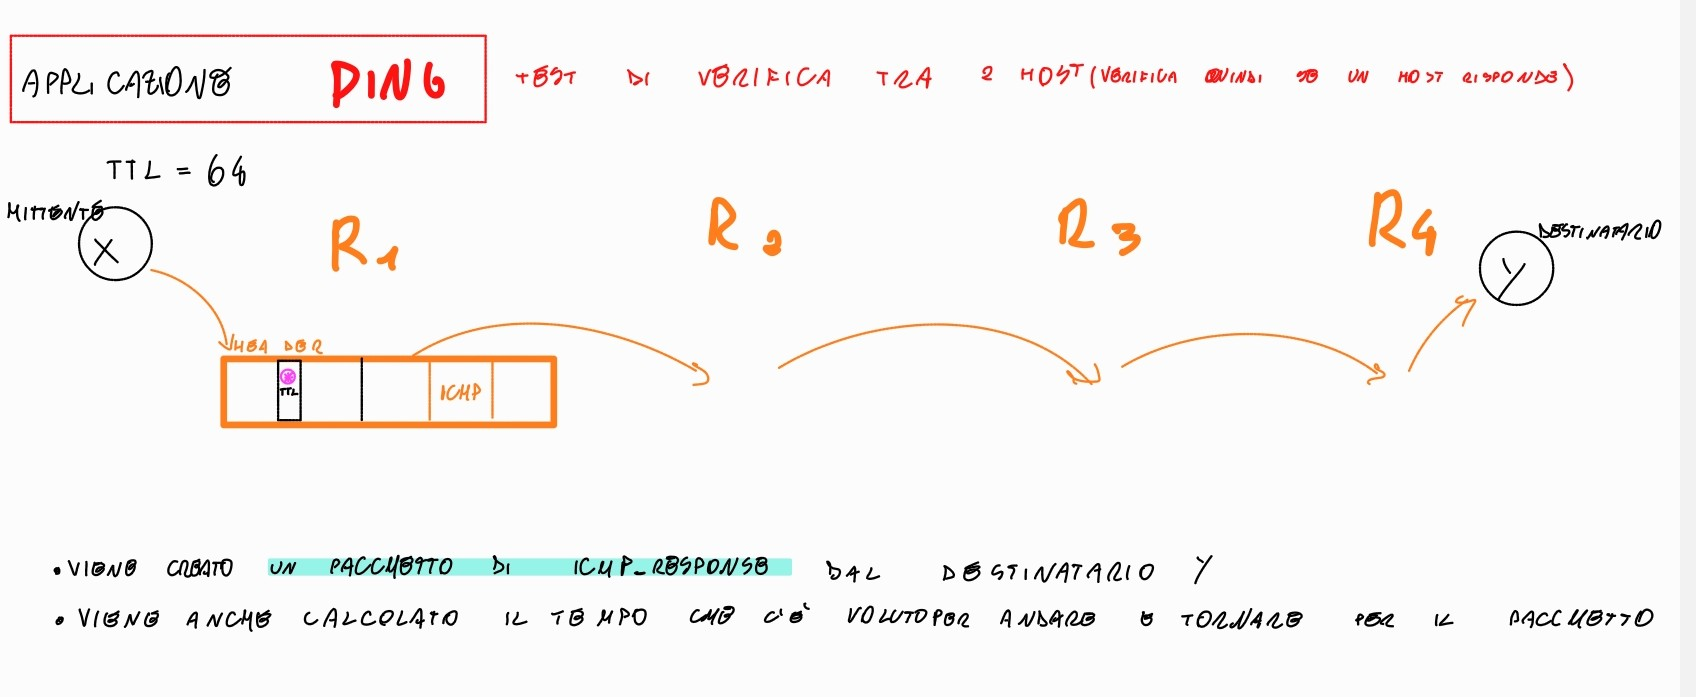
\includegraphics[width=0.9\linewidth]{foto reti di calcolatori/Ping.jpg}
    \caption{Dinamica di un PING: Invio della richiesta ICMP e ricezione della risposta con conseguente calcolo dell'RTT.}
    \label{fig:ping_schema}
\end{figure}

\begin{esempiobox}{Cosa succede se esegui PING nel terminale}
Se apri il prompt dei comandi e scrivi \texttt{ping www.google.com}, il tuo PC invierà di default 4 pacchetti (su Windows). Alla fine ti mostrerà le statistiche:
\begin{itemize}
    \item \textbf{Successo:} Vedrai righe come \texttt{Risposta da 142.250.180.132: byte=32 durata=15ms TTL=117}. Ti conferma che l'host esiste e ci ha messo 15 millisecondi a rispondere.
    \item \textbf{Richiesta scaduta (Timeout):} Il pacchetto è stato inviato, ma la risposta non è tornata indietro entro il tempo massimo previsto (es. 4 secondi). Può indicare problemi di rete, pacchetti persi o un firewall che blocca l'ICMP.
    \item \textbf{Host di destinazione irraggiungibile:} Il tuo router (o un router intermedio) ti avvisa che non sa proprio come trovare la strada per quell'indirizzo IP.
\end{itemize}
\end{esempiobox}

\newpage
\subsubsection*{Traceroute (o Tracert)}

Se il Ping ti dice \textit{se} puoi raggiungere una destinazione, il \textbf{Traceroute} ti dice \textit{quale strada} fanno i tuoi pacchetti per arrivarci, elencando tutti i router (hop) attraversati.

\textbf{Come funziona (Il trucco del TTL):}
Il Traceroute è un'applicazione geniale che sfrutta "a suo vantaggio" il meccanismo di distruzione dei pacchetti del campo \textbf{TTL (Time To Live)} dell'header IP.

\begin{enumerate}[leftmargin=*]
    \item Il tuo PC invia un pacchetto verso la destinazione, ma imposta volutamente il \textbf{TTL = 1}. 
    \item Il pacchetto arriva al \textbf{primo router} (il tuo modem di casa). Il router scala il TTL a 0, distrugge il pacchetto e ti invia un messaggio di errore ICMP \textit{Time Exceeded}. Ora tu sai l'indirizzo IP del tuo primo router!
    \item Il PC invia un secondo pacchetto, stavolta con \textbf{TTL = 2}. Questo sopravvive al primo router, ma muore sul \textbf{secondo router}, che ti risponde con un altro \textit{Time Exceeded}. Ora conosci il secondo passo.
    \item Il processo continua incrementando il TTL (3, 4, 5...) finché il pacchetto non riesce finalmente a raggiungere l'host di destinazione, il quale risponderà con un normale ICMP \textit{Echo Reply}. Il percorso è stato mappato.
\end{enumerate}

\begin{figure}[H]
    \centering
    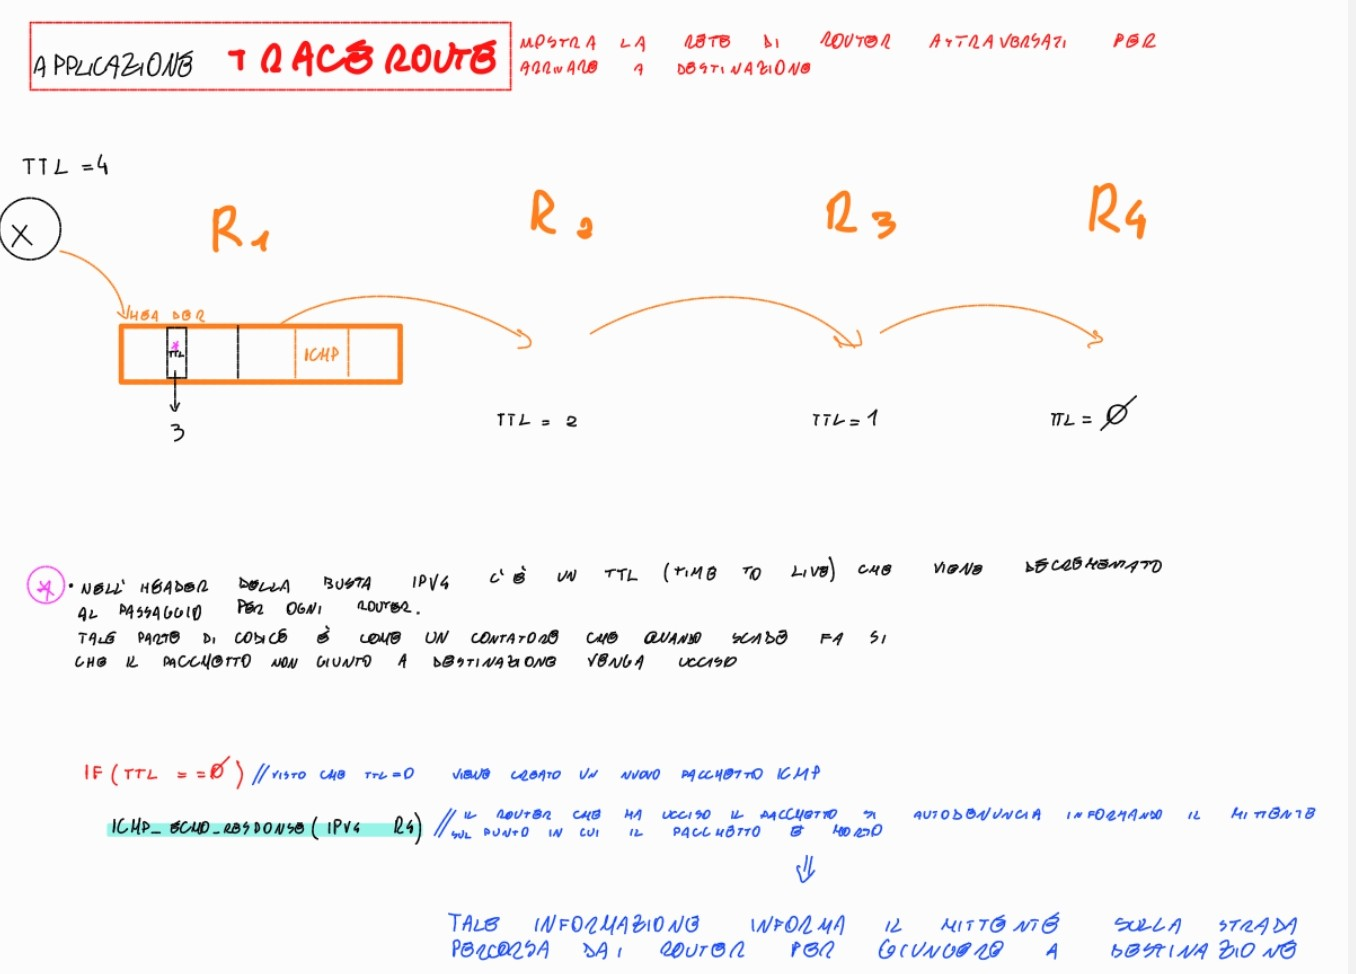
\includegraphics[width=1\linewidth]{foto reti di calcolatori/Traceroute.jpg}
    \caption{Funzionamento del Traceroute: incremento progressivo del TTL per forzare le risposte di errore ICMP da parte dei router intermedi.}
    \label{fig:traceroute_schema}
\end{figure}

\begin{esempiobox}{Cosa succede se esegui Traceroute nel terminale}
Se digiti \texttt{tracert www.google.com} (su Windows) o \texttt{traceroute www.google.com} (su Mac/Linux), vedrai apparire una lista numerata (1, 2, 3...).
\begin{itemize}
    \item Ogni riga rappresenta un \textbf{router intermedio}. Per ogni router vengono mostrati 3 valori di latenza (vengono inviati 3 pacchetti per sicurezza) e l'indirizzo IP del nodo.
    \item Se vedi degli \textbf{asterischi (* * *)}, significa che quel particolare router ha ignorato la richiesta (molti router commerciali sono configurati per non rispondere ai messaggi ICMP per motivi di sicurezza o risparmio energetico), ma il pacchetto ha comunque proseguito il suo viaggio.
\end{itemize}
\end{esempiobox}

\newpage
% ===============================================================
\subsection{Protocollo ARP e Reverse-ARP}

Quando un router deve consegnare un pacchetto IP a un host appartenente alla propria sottorete,
deve conoscere l'\textbf{indirizzo MAC} associato all'\textbf{indirizzo IP} di destinazione.
Questo perché la trasmissione sul segmento locale avviene mediante \textbf{frame MAC/LLC}, non
attraverso indirizzi IP.

Per risolvere l'associazione IP -> MAC viene utilizzato il protocollo
\textbf{ARP (Address Resolution Protocol)}.

\begin{itemize}
    \item Il router invia un \textbf{frame broadcast} con una richiesta ARP:  
          \textit{``Chi ha questo indirizzo IP? Mi mandi il tuo MAC?''}
    \item Tutti gli host della LAN ricevono il broadcast.
    \item Solo il destinatario corretto risponde con un frame unicast contenente il proprio MAC.
    \item Il router aggiorna la \textbf{cache ARP} e può costruire la busta MAC/LLC per consegnare il pacchetto.
\end{itemize}
\begin{defbox}{Funzione di ARP}
ARP è il protocollo che permette di collegare
\[
    \text{Indirizzo IP (livello rete)} \quad \longrightarrow \quad
    \text{Indirizzo MAC (livello MAC/LLC)}
\]
rendendo possibile il forwarding locale dei pacchetti IP.
\end{defbox}
\begin{notebox}{ARP processo sempre attivo a livello rete}
    ARP può essere visto come un meccanismo sempre attivo nel livello rete, che opera con una
logica molto semplice, assimilabile a una struttura di controllo \textit{if–then–else}:

\begin{itemize}
    \item \textbf{IF} l’associazione IP $\rightarrow$ MAC \textbf{è già presente} nella cache ARP  

    
          \textbf{THEN} il router utilizza direttamente il MAC memorizzato per costruire il frame MAC/LLC
          e inoltra immediatamente il pacchetto.

    \item \textbf{ELSE} (l’associazione non è presente)  
          il router deve \textbf{richiederla dinamicamente} inviando un frame ARP \textbf{in broadcast} sulla LAN:
          \[
              \text{``Chi ha questo indirizzo IP?''}
          \]
          Il dispositivo corretto risponde con il proprio MAC, la cache ARP viene aggiornata e il router
          può finalmente preparare il frame MAC/LLC.
\end{itemize}

In altre parole, ARP non cerca sempre da zero il MAC di destinazione: prima controlla la memoria
locale (\textbf{cache ARP}). Solo se l’informazione non è disponibile, attiva il meccanismo di
risoluzione tramite broadcast. Per questo possiamo dire che ARP si comporta come un
\textbf{controllo condizionale continuo} nel livello rete.

\end{notebox}

\begin{notebox}{RARP}
Il protocollo \textbf{Reverse ARP (RARP)} risponde alla domanda inversa:

\begin{center}
\textit{``Quale indirizzo IP appartiene a questo indirizzo MAC?''}
\end{center}

È stato utilizzato storicamente da macchine senza disco per ottenere il proprio IP,
ma oggi è stato sostituito da BOOTP e DHCP.
\end{notebox}

\subsubsection{Esempio: consegna di un pacchetto IP tramite ARP}

\begin{figure}[H]
    \centering
    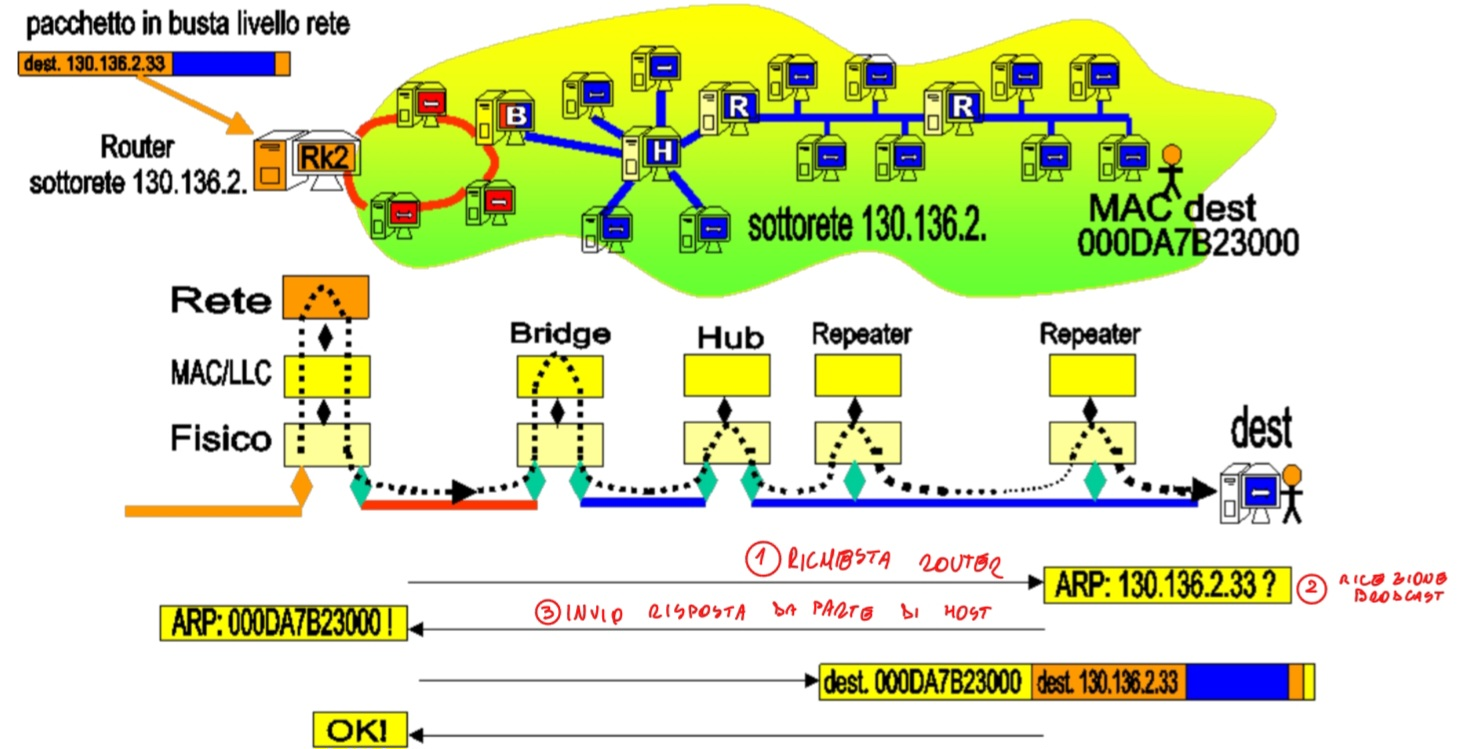
\includegraphics[width=0.8\linewidth]{foto reti di calcolatori/ARP.jpg}
    \label{fig:placeholder}
\end{figure}

Si consideri un router che riceve un pacchetto IP destinato all'host
\texttt{130.136.2.33}, appartenente alla sua sottorete locale.

Il router deve trasformare il pacchetto IP in un \textbf{frame MAC/LLC} indirizzato
al MAC del destinatario. Tuttavia, se l'associazione IP–MAC non è presente nella cache ARP,
il router procede come segue:

\begin{enumerate}
    \item Il router invia sulla LAN un \textbf{frame in broadcast} con una richiesta ARP:
    \[
        \text{``Chi ha l'indirizzo IP \texttt{130.136.2.33}?''}
    \]
    
    \item Tutti i dispositivi della sottorete ricevono il broadcast.

    \item L'host con IP \texttt{130.136.2.33}, se esiste, risponde con un
          \textbf{frame unicast} diretto al MAC del router, contenente:
          \[
          \text{Risposta ARP + indirizzo MAC dell'host}
          \]

    \item Il router aggiorna la propria \textbf{cache ARP}.

    \item A questo punto può incapsulare il pacchetto IP in un frame MAC/LLC:
          \[
          \text{MAC sorgente = MAC del router} \qquad
          \text{MAC destinazione = MAC dell’host}
          \]

    \item L'host riceve il frame e invia un \textbf{frame di conferma} al sottolivello LLC.
\end{enumerate}

\begin{notebox}{Ruolo di ARP nella rete locale}
ARP lega l'indirizzamento IP (livello rete) con l'indirizzamento MAC
(livello MAC/LLC).  
Senza ARP, un router non potrebbe mai consegnare un pacchetto IP a un host
della propria rete locale.
\end{notebox}


\newpage
% ===============================================================
\subsection{Assegnazione degli indirizzi IP: statica o tramite  DHCP}
L’ assegnazione degli indirizzi IP avviene su due livelli distinti:

\begin{enumerate}
    \item \textbf{Assegnazione dei numeri di rete}
    
    La parte sinistra degli indirizzi IP (classi A, B, C) viene assegnata a enti, aziende e organizzazioni
    da parte di organismi internazionali come \textbf{RIPE, ICANN, ARIN, APNIC}.  
    Queste porzioni di indirizzi rappresentano il dominio amministrativo gestito dall'organizzazione.

    \item \textbf{Assegnazione dei numeri di host}
    
    È la parte più pratica: riguarda l’assegnazione degli indirizzi IP ai dispositivi di una rete locale.
\end{enumerate}

\subsubsection*{Modalità di assegnazione degli indirizzi IP agli host}

\begin{itemize}
    \item \textbf{Assegnazione statica}  
    E' l'amministratore di rete associa manualmente a un dispositivo:
    \begin{itemize}
        \item un \textbf{indirizzo IP} libero della rete;
        \item il \textbf{MAC dell’interfaccia} corrispondente.  
    \end{itemize}
    Questa associazione è permanente: l’indirizzo IP rimane invariato nel tempo.

    \item \textbf{Assegnazione dinamica (DHCP)}  
    La modalità più diffusa in reti wireless, LAN aziendali, reti domestiche.
    Avviene tramite un server \textbf{DHCP (Dynamic Host Configuration Protocol\footnote{Questo è un protocollo di livello applicazione descritto nella sezione \ref{sec:DHCP} })}.
\end{itemize}



\begin{notebox}{DHCP fornisce più di un indirizzo IP}
Il \textbf{server DHCP}:
\begin{itemize}
    \item mantiene una lista di \textbf{host number liberi} per la sottorete amministrata;
    \item assegna dinamicamente indirizzi IP ai dispositivi che lo richiedono;
    \item associa un indirizzo IP a un indirizzo MAC per la durata del \textit{lease};
    \item può configurare automaticamente anche:
    \begin{itemize}
        \item maschera di rete (subnetmask),
        \item default gateway,
        \item indirizzo server DNS.
    \end{itemize}
\end{itemize}
\end{notebox}


\begin{notebox}{Perché DHCP?}
Il protocollo DHCP fornisce un servizio di rete “\textbf{plug and play}”:  
basta connettere un dispositivo e questo ottiene \textbf{automaticamente} tutti i parametri necessari al funzionamento nella rete.

\vspace{0.5cm}
Vantaggi di DHCP:
\begin{itemize}
    \item \textbf{Riuso degli indirizzi}: gli indirizzi vengono assegnati
          con un \textit{lease} temporaneo -- quando un host si
          disconnette, l'indirizzo ritorna disponibile nel pool del server.
    \item \textbf{Mobilità}: un host che si sposta in una rete diversa
          ottiene automaticamente un indirizzo valido per quella rete.
    \item \textbf{Gestione centralizzata}: un solo server DHCP gestisce
          tutta la configurazione di rete della subnet.
\end{itemize}
\end{notebox}

\newpage
% ==================================================================
\subsubsection*{Esempio: funzionamento di un DHCP server}

\begin{esempiobox}{Assegnazione dinamica degli indirizzi IP}
Si consideri un DHCP server per la rete \texttt{140.136.2.x}.  
Il server mantiene una lista di \textbf{host number}
disponibili nella sottorete: [10, 11, 12, 13, 14, 15]

Tre dispositivi con indirizzi MAC:
\[
\texttt{MAC1},\quad \texttt{MAC2},\quad \texttt{MAC3}
\]
inviando una richiesta DHCP ottengono rispettivamente gli host number:
\[
10,\quad 13,\quad 14.
\]

Gli indirizzi IP assegnati diventano:
\[
\texttt{140.136.2.10},\quad
\texttt{140.136.2.13},\quad
\texttt{140.136.2.14}.
\]

La lista del DHCP server viene aggiornata e risultano ancora liberi gli host number:
\[
11,\ 12,\ 15,\dots
\]
per future assegnazioni dinamiche.
\end{esempiobox}

\subsubsection{Funzionamento del processo DHCP: client e server}

Il processo di assegnazione dinamica di un indirizzo IP mediante DHCP è basato su uno 
scambio di messaggi tra \textbf{client} e \textbf{server} usando il protocollo \textbf{UDP}.

\begin{itemize}
    \item Il \textbf{client DHCP} utilizza la porta \textbf{UDP 68}.
    \item Il \textbf{server DHCP} utilizza la porta \textbf{UDP 67}.
\end{itemize}

Questa distinzione permette al server di riconoscere le richieste provenienti dai client 
e ai client di ricevere le risposte anche quando non hanno ancora un indirizzo IP valido.

\begin{figure}[H]
    \centering
    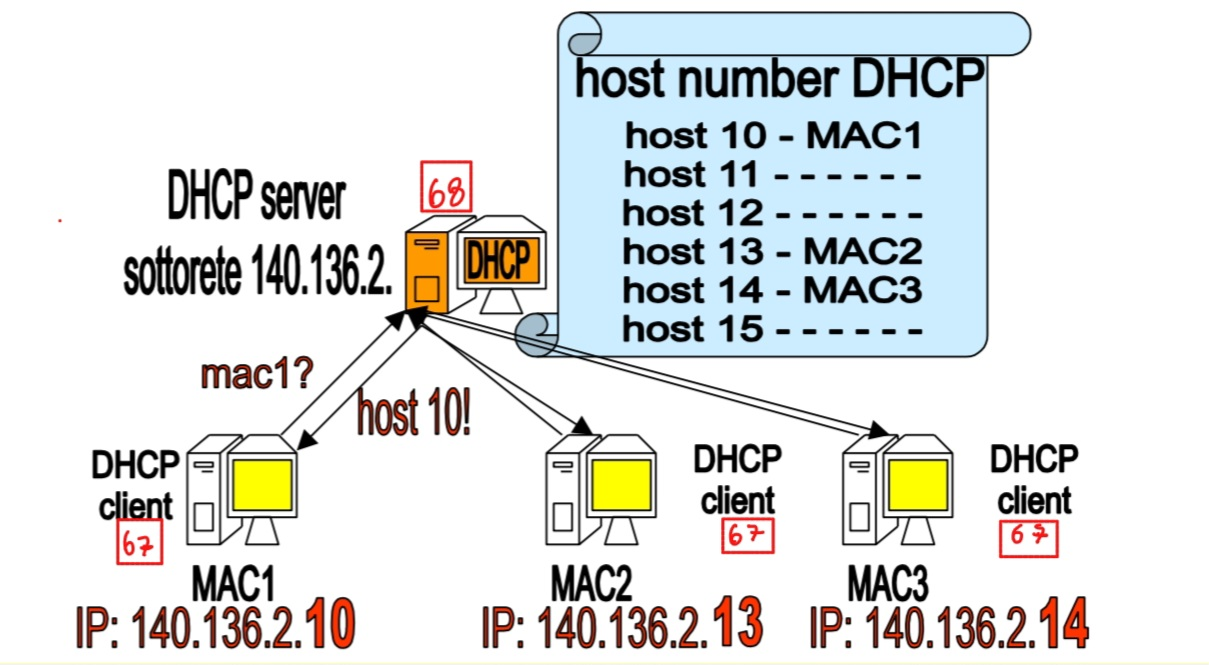
\includegraphics[width=0.6\linewidth]{foto reti di calcolatori/DHCP.jpg}
    \label{fig:placeholder}
\end{figure}



\subsubsection{Protocollo DHCP -- 4 passi}

\begin{figure}[H]
\centering
\begin{tikzpicture}[
    arrow/.style={->, thick},
    msg/.style={rectangle, draw, fill=yellow!20, align=center,
                font=\small, inner sep=4pt}
]
\draw[thick] (0, 0) -- (0, -8);
\draw[thick] (8, 0) -- (8, -8);
\node[font=\bfseries] at (0, 0.4) {Client};
\node[font=\bfseries] at (8, 0.4) {Server DHCP};

\draw[arrow, blue] (0, -1) -- (8, -1.5);
\node[msg, fill=blue!10] at (4, -0.9) {%
    \textbf{DHCP Discover}\\
    src: \texttt{0.0.0.0:68},
    dst: \texttt{255.255.255.255:67}\\
    ``C'è un server DHCP?''};

\draw[arrow, green!60!black] (8, -3) -- (0, -3.5);
\node[msg, fill=green!10] at (4, -2.7) {%
    \textbf{DHCP Offer}\\
    src: \texttt{168.1.1.1:67},
    dst: \texttt{255.255.255.255:68}\\
    yiaddr: \texttt{168.1.1.10}, lifetime: 3600s};

\draw[arrow, orange] (0, -5) -- (8, -5.5);
\node[msg, fill=orange!10] at (4, -4.7) {%
    \textbf{DHCP Request}\\
    src: \texttt{0.0.0.0:68},
    dst: \texttt{255.255.255.255:67}\\
    ``Prendo quell'indirizzo!''};

\draw[arrow, red!70!black] (8, -7) -- (0, -7.5);
\node[msg, fill=red!10] at (4, -6.7) {%
    \textbf{DHCP ACK}\\
    src: \texttt{168.1.1.1:67},
    dst: \texttt{255.255.255.255:68}\\
    Indirizzo confermato + DNS + gateway};
\end{tikzpicture}
\caption{%
    \textbf{I 4 passi del protocollo DHCP (schema DORA).}
    Tutti i messaggi usano il \textbf{broadcast}
    (\texttt{255.255.255.255}) perché il client non ha ancora
    un indirizzo IP valido -- non potrebbe inviare messaggi
    unicast.
}
\label{fig:dhcp}
\end{figure}


\begin{enumerate}
    \item \textbf{DHCP Discover} (client → server)  
    Il client (ovvero un host nuovo), senza IP, invia un pacchetto \textbf{broadcast}:
    
    MAC:
    \[
    \text{Mittete: MAC mittente; Destinatario:: ff:ff:ff:ff:ff:ff, }
    
    \]
    Non conoscendo inoltre l'indirizzo IP:
    \[    
    \text{Mittente: 000.000.000.000; Destinatario (brodcast): 255.255.255.255}
    \]
    verso la porta UDP 67.  
    
    Il messaggio serve a cercare un DHCP server disponibile nella rete.

    \item \textbf{DHCP Offer} (server → client)  
    Un server DHCP che riceve il Discover risponde con un’offerta, contenente:
    \begin{itemize}
        \item un indirizzo IP proposto,
        \item la durata del lease,
        \item la subnet mask,
        \item eventuali DNS e gateway.
    \end{itemize}
    L' offerta viene inviata spesso ancora in broadcast (il client non ha IP assegnato).

    \item \textbf{DHCP Request} (client → server)  
    Il client seleziona una delle offerte ricevute  e invia un messaggio
    DHCP Request in broadcast per comunicare:
    \[
    \text{``Accetto l'offerta del server X. Voglio l’indirizzo Y.''}
    \]
    Questo meccanismo evita che due server credano di essere stati accettati.

    \item \textbf{DHCP ACK} (server → client)  
    Il server conferma l’assegnazione e invia un ACK contenente:
    \begin{itemize}
        \item l’indirizzo IP finale,
        \item la maschera di rete,
        \item il router predefinito,
        \item il DNS,
        \item il tempo di lease.
    \end{itemize}
    Da questo momento il client può usare l’indirizzo IP assegnato.
\end{enumerate}

\begin{notebox}{Riepilogo essenziale}
\textbf{Porta 67 (server DHCP)}: ascolta richieste dei client. \\
\textbf{Porta 68 (client DHCP)}: riceve risposte dal server. \\
\textbf{Discover $\rightarrow$ Offer $\rightarrow$ Request $\rightarrow$ ACK}: ciclo completo di assegnazione IP.
\end{notebox}

\begin{collegamentobox}[title=�� ESEMPIO:  (Cap. 5) sezione 5.3.5 DHCP]
    In questa sezione è presente un ulteriore esercizio riguardande un esempio di vita reale
\end{collegamentobox}
% ===============================================================
% IPv6 E TUNNELLING
% ===============================================================
\newpage
\subsection{IPv6 e Tunnelling IPv4/IPv6}
\footnote{Se si vuole c'è una speiagzione simile anche nella sezione  5.3.7 capitolo 5 riguardo al Tunneling}
L’evoluzione di Internet e la crescita esponenziale del numero di dispositivi connessi hanno portato,
sin dagli anni ’90, alla necessità di introdurre una nuova versione del protocollo IP.


Per risolvere questo problema è stato introdotto il \textbf{protocollo IPv6}, la nuova generazione
dell’indirizzamento a livello rete, progettata per garantire scalabilità, efficienza e supporto a nuove
tecnologie.

\subsubsection*{Caratteristiche fondamentali di IPv6}

\begin{itemize}
    \item \textbf{Indirizzi a 128 bit (16 byte)}: quattro volte più grandi dei 32 bit di IPv4 (4byte).  
    \item \textbf{Nuova struttura dell’intestazione IP}:  
          Sono state introdotte etichette numeriche utili per la gestione ottimizzata di flussi di dati con priorità differenti.

          Inoltre grazie alla maggiore affidabilità della rete non viene fatta frammentazione
\end{itemize}

Nonostante i vantaggi, IPv6 non è direttamente compatibile con i router IPv4: la maggior parte
dell’attuale Internet si basa ancora su infrastrutture IPv4, rendendo necessarie tecniche di
\textbf{transizione}.

\subsubsection*{Tecniche di transizione: il tunnelling IPv6 in IPv4}

Una delle tecniche più diffuse è il \textbf{tunnelling}: pacchetti IPv6 vengono incapsulati dentro pacchetti
IPv4, permettendo loro di attraversare tratte di rete che supportano solo IPv4.

\begin{figure}[H]
    \centering
    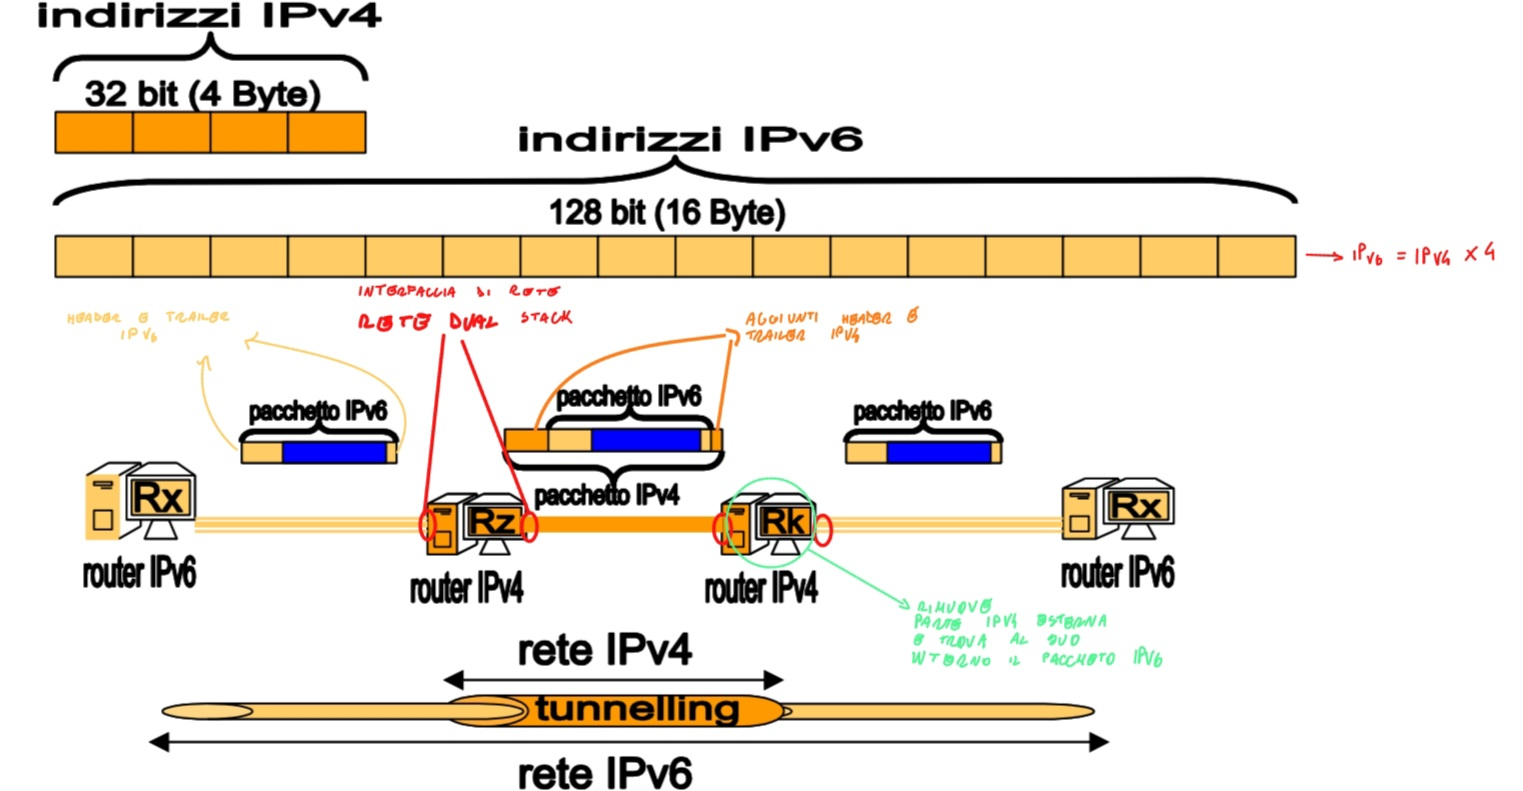
\includegraphics[width=1\linewidth]{foto reti di calcolatori/tunneling.jpg}
    \caption{Confronto tra indirizzi IPv4 (32 bit) e IPv6 (128 bit) e esempio di tunnelling IPv6 incapsulato in pacchetti IPv4.}
\end{figure}

Il principio operativo è semplice:

\begin{enumerate}
    \item Un router IPv6 vuole inviare un pacchetto a un altro router IPv6 distante.
    \item Parte del cammino è composta da router che hanno interfaccia di rete dual stack ( 2 schede di rete con due protocolli differenti: IPv6 da un lato e IPv4 dall'altro). Tali router hanno delle tabelle di instradamento ibride
    \item Il router IPv4 incapsula il pacchetto IPv6 dentro un normale pacchetto IPv4.
    \item I router IPv4 inoltrano il pacchetto come se fosse un normale pacchetto IPv4.
    \item All’uscita della parte IPv4, un router specializzato estrae il pacchetto IPv6 originale.
\end{enumerate}

\begin{notebox}{Integrazione IPv4 e IPv6}
IPv6 non sostituisce immediatamente IPv4: la transizione avviene gradualmente tramite meccanismi di compatibilità.
Il tunnelling permette agli host IPv6 di comunicare tra loro anche in una rete che contiene tratte IPv4.
\end{notebox}


\begin{notebox}{Confronto Architetturale: Instradamento e Sottoreti in IPv4 vs IPv6}
L'evoluzione da IPv4 a IPv6 ha comportato un radicale cambiamento nella gestione degli indirizzi e dell'instradamento, passando da una complessa frammentazione a una struttura più lineare.

\textbf{IPv4: Struttura Gerarchica e Sottoreti} \\
A livello logico, IPv4 utilizza una struttura fortemente gerarchica in cui una rete principale viene frammentata in sottoreti più piccole.
\begin{itemize}
    \item \textbf{Funzionamento:} L'instradamento procede per step: il pacchetto arriva al router della rete principale, viene inoltrato al router della sottorete di competenza e, infine, tramite il protocollo ARP viene individuato il MAC address dell'host finale.
    \item \textbf{Pregi:} Permette di organizzare gerarchicamente le macchine e di contenere il traffico locale (broadcast) all'interno di domini isolati.
    \item \textbf{Difetti:} L'esaurimento del limitato spazio di indirizzamento a 32 bit  ha costretto all'uso massiccio del CIDR  e del NAT\footnote{Vedi sezione \ref{NAT}}. Questo aumenta enormemente il carico di lavoro sui router e viola il principio architetturale della comunicazione diretta end-to-end.
\end{itemize}

\vspace{0.5cm}
\textbf{IPv6: Struttura Semplificata e Instradamento Globale} \\
IPv6 non prevede la gestione delle sottoreti con la stessa complessa logica di IPv4.
\begin{itemize}
    \item \textbf{Funzionamento:} La struttura è molto più piatta. L'enorme disponibilità di indirizzi a 128 bit  permette un'allocazione logica che semplifica radicalmente le tabelle di instradamento.
    \item \textbf{Pregi:} Riduce il carico computazionale all'interno dei router garantendo un instradamento globale estremamente efficiente. Inoltre, eliminando la necessità del NAT, ripristina la reale comunicazione end-to-end tra sistemi distanti.
    \item \textbf{Difetti:} L'infrastruttura di Internet è ancora prevalentemente basata su IPv4; questo obbliga all'uso di complesse tecniche di transizione, come il \textit{tunnelling} (incapsulamento di pacchetti IPv6 dentro buste IPv4), per attraversare i router che non supportano il nuovo protocollo.
\end{itemize}
\end{notebox}

\newpage


%================
\newpage

\subsection{NAT: Network Address Translation}
\label{NAT}
\begin{defbox}{NAT}
\textbf{NAT} (\textit{Network Address Translation}) è una
tecnica per cui un router di confine traduce gli indirizzi IP:
la rete locale usa un blocco di indirizzi \textbf{privati}
(non routable su Internet, es.\ \texttt{10.0.0.0/8}), e tutti
i datagrammi che escono dalla rete locale vengono tradotti
per usare un \textbf{unico} indirizzo IP pubblico assegnato
dall'ISP.
\end{defbox}

\subsubsection{Motivazioni e Vantaggi}
L'adozione del NAT è motivata da diversi fattori pratici:
\begin{itemize}
    \item \textbf{Risparmio di indirizzi IP:} Non è necessario un range di indirizzi pubblici dall'ISP; basta un solo IP per tutti i dispositivi (computer, telefoni, smart TV) della casa o dell'ufficio.
    \item \textbf{Flessibilità locale:} È possibile cambiare gli indirizzi dei dispositivi interni senza notificare il mondo esterno.
    \item \textbf{Flessibilità ISP:} È possibile cambiare fornitore di servizi (e quindi IP pubblico) senza dover riconfigurare gli indirizzi IP di tutti i dispositivi interni.
    \item \textbf{Sicurezza:} I dispositivi interni non sono direttamente indirizzabili o visibili dall'esterno, offrendo una protezione naturale contro le connessioni non richieste.
\end{itemize}

\subsubsection{Implementazione: La Tabella di Traduzione}
Il \textbf{router NAT} deve gestire la corrispondenza tra le molteplici connessioni interne e l'unica uscita pubblica. Per farlo, utilizza una \textbf{NAT Translation Table} e manipola i numeri di \textbf{porta}.

Il router esegue le seguenti operazioni:
\begin{enumerate}
    \item \textbf{In uscita (Outgoing):} Sostituisce la coppia \texttt{(IP sorgente, Porta)} del datagramma interno con una nuova coppia \texttt{(IP NAT, Nuova Porta)} univoca.
    \item \textbf{Memorizzazione:} Salva questa associazione nella tabella di traduzione NAT.
    \item \textbf{In entrata (Incoming):} Quando riceve una risposta destinata a \texttt{(IP NAT, Nuova Porta)}, consulta la tabella per trovare l'IP e la porta interni originali e sostituisce i campi nel datagramma prima di inoltrarlo alla LAN.
\end{enumerate}

\newpage
\begin{esempiobox}{Esempio Passo-Passo: Host $\to$ Web Server}
    Immaginiamo un host interno \texttt{10.0.0.1} che vuole contattare un server web esterno \texttt{128.119.40.186}. Il router NAT ha IP pubblico \texttt{138.76.29.7}.

    \begin{itemize}
        \item \textbf{Passo 1 (Invio / datagramma in uscita - da rete locale ad internet):} L'host invia un datagramma.
        \\ \textit{Sorgente:} \texttt{10.0.0.1, 3345} $\to$ \textit{Destinazione:} \texttt{128.119.40.186, 80}
        \\ \textit{(Nota: Poiché l'IP di destinazione non appartiene alla sottorete locale, l'host invia il pacchetto al Default Gateway, ovvero il router).}
        
        \item \textbf{Passo 2 (Traduzione Router):} Il router riceve il datagramma sull'interfaccia LAN. Poiché deve inoltrarlo verso la rete esterna (WAN), applica il NAT:
        \begin{itemize}
            \item Sostituisce l'IP sorgente privato (\texttt{10.0.0.1}) con il proprio IP pubblico (\texttt{138.76.29.7}).
            \item Sostituisce la porta sorgente (\texttt{3345}) con una nuova porta libera scelta arbitrariamente (es. \texttt{5001}) per identificare univocamente questa sessione.
            \item \textbf{Aggiornamento Tabella:} Aggiunge una riga alla tabella NAT: \texttt{\{138.76.29.7, 5001\} $\leftrightarrow$ \{10.0.0.1, 3345\}}.
        \end{itemize}
        \textit{Nuovo Datagramma:} \texttt{138.76.29.7, 5001} $\to$ \texttt{128.119.40.186, 80}
        
        \item \textbf{Passo 3 (Risposta Server):} Il server web elabora la richiesta e risponde all'indirizzo pubblico del router.
        \\ \textit{Sorgente:} \texttt{128.119.40.186, 80} $\to$ \textit{Destinazione:} \texttt{138.76.29.7, 5001}
        
        \item \textbf{Passo 4 (Inoltro / datagramma in entrata ):} Il router riceve il pacchetto sulla porta \texttt{5001}. Consulta la tabella NAT per la traduzione inversa: \texttt{5001} corrisponde all'host interno \texttt{10.0.0.1} sulla porta \texttt{3345}. Il router modifica l'intestazione e inoltra il pacchetto nella LAN.
    \end{itemize}
\end{esempiobox}

\begin{figure}[H]
    \centering
    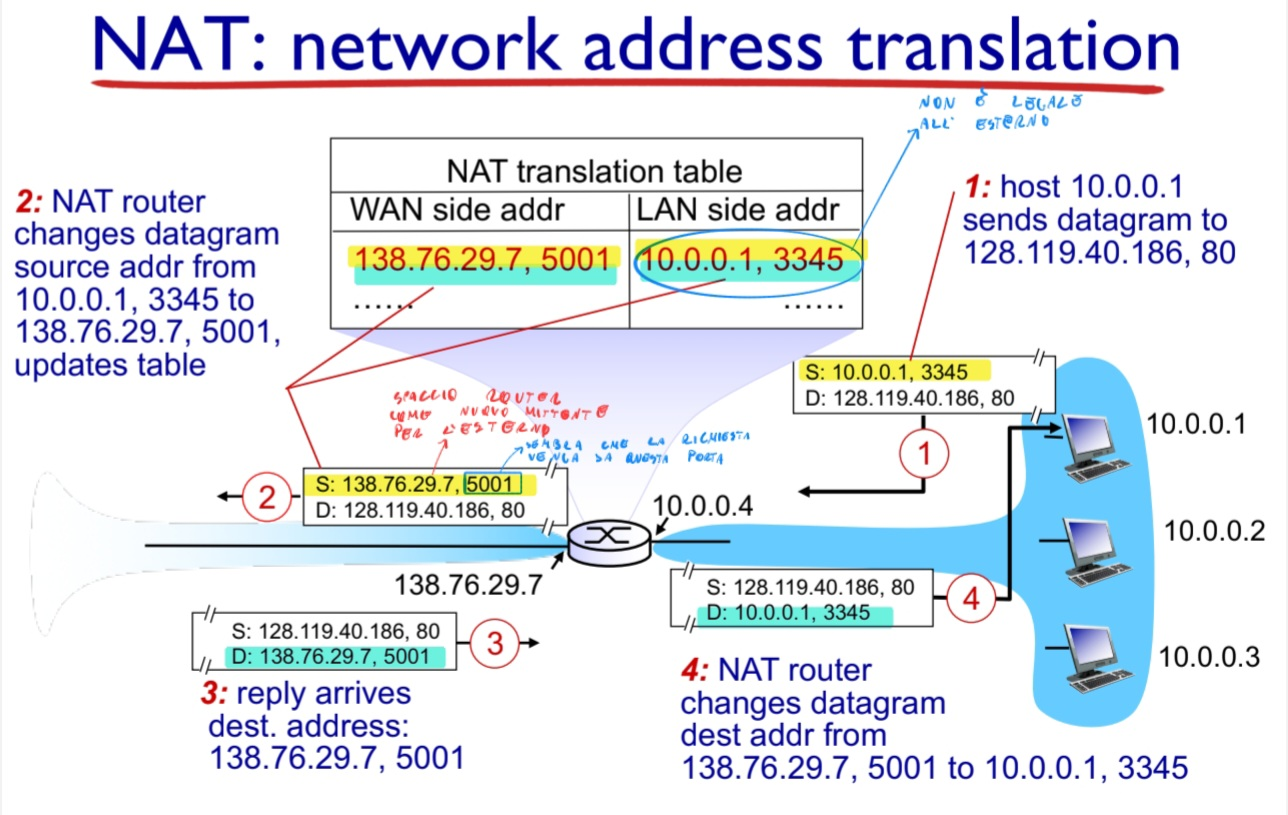
\includegraphics[width=0.8\linewidth]{foto reti di calcolatori/NAT.jpg}
    \caption{rappresentazione Router NAT a cui è associata una tabella dii traduzione NAT. Nella figura abbiamo a destra del router la local network (ad esempio la rete di casa), a sinistra abbiamo il resto di internet }
    \label{fig:placeholder}
\end{figure}


\newpage
\subsubsection{Limiti e Controversie}
Nonostante la sua utilità, il NAT è oggetto di critiche architetturali:
\begin{itemize}
    \item \textbf{Violazione dei livelli:} I router dovrebbero processare solo fino al livello 3 (Rete/IP), mentre il NAT manipola le porte (livello 4 Trasporto).
    \item \textbf{Violazione End-to-End:} L'argomento "end-to-end" sostiene che gli host dovrebbero comunicare direttamente senza intermediari che modificano i pacchetti.
    \item \textbf{Problemi con P2P:} Applicazioni Peer-to-Peer richiedono che i client siano contattabili dall'esterno, cosa che il NAT impedisce (richiede tecniche complesse di \textit{NAT traversal}).
    \item \textbf{IPv6:} La carenza di indirizzi IP (il motivo principale del NAT) dovrebbe essere risolta nativamente adottando IPv6, rendendo il NAT obsoleto.
\end{itemize}



\begin{notebox}{Scalabilità}
    Il campo del numero di porta è a 16-bit. Questo significa che un singolo indirizzo IP pubblico (lato WAN) può gestire oltre \textbf{60.000 connessioni simultanee} provenienti dalla rete locale (lato LAN).
    È improbabile che i dispositivi di una rete domestica generino contemporaneamente un numero di connessioni tale da saturare la tabella NAT.
\end{notebox}

\begin{collegamentobox}[title=�� ESEMPIO:  (Cap. 5) sezione 5.3.6 Aggregazione gerarchica tramite NAT]
    In questa sezione è presente un ulteriore esercizio riguardande un esempio di vita reale
\end{collegamentobox}

\newpage
\subsection{Funzioni di Port Mapping e Port Filtering (Traffico iniziato dall'esterno)}

Il NAT puro blocca di default qualsiasi connessione iniziata dall'esterno verso l'interno, poiché il router non ha modo di sapere a quale dispositivo della rete locale (LAN) recapitare i pacchetti "non richiesti". Per permettere a un host esterno di raggiungere una macchina interna (es. per ospitare un server o accedere a una videocamera), si utilizzano due meccanismi complementari.

\subsubsection*{Dettaglio dei Meccanismi}

\begin{itemize}
    \item \textbf{Port Mapping (Port Forwarding o DNAT):} Risponde alla domanda \textit{"A chi lo consegno?"}. Agisce come un instradatore, creando una regola statica nel router che mappa una specifica porta pubblica verso una destinazione interna definita dalla tripla \texttt{[IP\_Privato\_Dest, Porta\_Privata\_Dest, Protocollo]}. Senza questa associazione, il pacchetto in arrivo sull'IP pubblico sbatte contro un "muro" e viene scartato.
    
    \item \textbf{Port Filtering (Firewall):} Risponde alla domanda \textit{"Chi è autorizzato a entrare?"}. È il controllo di sicurezza all'ingresso. Verifica le regole impostate dall'amministratore (es. le Access Control List) per decidere se la porta è \textit{aperta} o \textit{chiusa} per quel determinato traffico. Se configurato su \texttt{DROP} o \texttt{DENY}, la richiesta viene distrutta a monte, rendendo di fatto inapplicabile anche la regola di mapping successiva.
\end{itemize}

\begin{esempiobox}{Esempio pratico: Ospitare un Server Web in casa}
   Immaginiamo di avere un server web nella nostra LAN con indirizzo IP privato \texttt{192.168.1.50} in ascolto sulla porta \texttt{80}. Il nostro router ha l'IP pubblico \texttt{82.50.10.20}.
  
  \textbf{1. Configurazione del Port Mapping:}
  Impostiamo una regola sul router: \textit{"Tutto il traffico TCP in arrivo sulla porta pubblica \texttt{8080}, deve essere inoltrato all'IP \texttt{192.168.1.50} sulla porta locale \texttt{80}"}.
  
  \textbf{2. Configurazione del Port Filtering (Sicurezza):}
  Per evitare attacchi informatici, impostiamo una regola sul firewall: \textit{"Consenti l'ingresso sulla porta pubblica \texttt{8080} SOLO agli IP sorgenti provenienti dall'Italia. Applica un \texttt{DROP} a tutti gli altri"}.
  
  \textbf{Cosa succede quando un utente dall'estero tenta di connettersi?}
  Il pacchetto arriva all'IP \texttt{82.50.10.20:8080}. Esiste una regola di Mapping valida, ma il Filtering interviene per primo: nota l'IP estero e distrugge il pacchetto. Il server interno è salvo.
\end{esempiobox}

\subsubsection*{Flusso Logico del Pacchetto in Ingresso}

Possiamo schematizzare il percorso sequenziale di un pacchetto proveniente da Internet verso un servizio locale:

\begin{enumerate}
    \item \textbf{Richiesta Esterna:} Il pacchetto arriva all'IP Pubblico del Router sulla porta specificata.
    \item \textbf{Port Filtering:} Il firewall verifica i permessi di sicurezza (Il traffico da questo mittente è consentito o va bloccato?).
    \item \textbf{Port Mapping:} Se il firewall autorizza il passaggio, il NAT consulta la sua tabella statica (A quale IP privato e a quale porta locale devo inoltrare questa porta pubblica?).
    \item \textbf{Inoltro (Forwarding):} L'intestazione del pacchetto viene modificata (sostituendo IP e porta di destinazione pubblica con quelli privati) e inviata al dispositivo interno corretto.
\end{enumerate}

\newpage
\subsection{Conclusioni}
Il livello di rete svolge un ruolo fondamentale nel garantire il corretto trasferimento dei pacchetti attraverso una rete complessa e potenzialmente eterogenea. 

La sua funzione principale è quella di determinare il percorso più appropriato che ciascun pacchetto deve seguire per raggiungere la destinazione, indipendentemente dalla posizione geografica o dalla struttura fisica della rete.

Durante l'attraversamento dei vari nodi intermedi, i pacchetti vengono temporaneamente memorizzati nei buffer dei router, i quali operano secondo una logica \textit{store-and-forward}: ogni router riceve il pacchetto, lo conserva nel proprio buffer e successivamente decide verso quale interfaccia inoltrarlo. 

Tale decisione si basa sulle tabelle di instradamento, strutture dati aggiornate dinamicamente che contengono le informazioni necessarie per scegliere il prossimo passo ottimale.  




% ===============================================================
% INIZIO DEL LIVELLO TRASPORTO
% ===============================================================
\newpage
\section{Livello Trasporto (4)}

Il \textbf{livello Trasporto} fornisce servizi di comunicazione logica tra processi applicativi su host diversi.
A differenza del livello Rete, che gestisce il percorso fisico dei pacchetti, il Trasporto si occupa di
stabilire un canale affidabile (o non affidabile) tra due applicazioni.

i pacchetti a questo livello vengono chiamati segmenti (\textcolor{red}{busta rossa})


I due protocolli fondamentali sono:

\begin{itemize}
    \item \textbf{UDP} — semplice, veloce e non affidabile;
    \item \textbf{TCP} — complesso, affidabile e orientato alla connessione.
\end{itemize}

\begin{figure}[H]
    \centering
    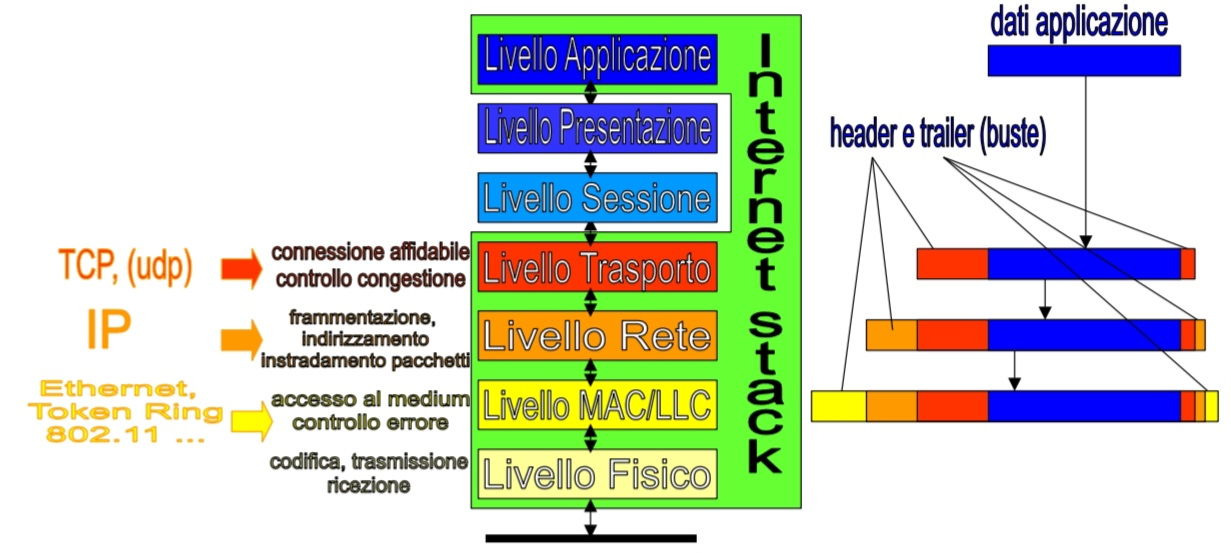
\includegraphics[width=0.9\linewidth]{foto reti di calcolatori/architettura.jpg}
    \caption{Livello Trasporto tra Applicazione e Rete: i protocolli TCP e UDP.}
\end{figure}

% ===============================================================
\subsection{UDP e TCP}







\subsubsection*{UDP: servizio non affidabile}

UDP fornisce un servizio di trasporto estremamente leggero:

\begin{defbox}{UDP -- User Datagram Protocol}
L’\textbf{UDP} è un protocollo di trasporto \textit{non orientato alla connessione}.  
Le sue caratteristiche principali sono:
\begin{itemize}
    \item \textbf{connectionless};
    \item non garantisce consegna, ordine né unicità dei pacchetti;
    \item non effettua ritrasmissioni;
    \item non controlla la congestione;
    \item overhead minimo.
\end{itemize}
\end{defbox}


\begin{esempiobox}{Quando usare UDP}
\begin{itemize}
    \item Streaming audio/video (serve velocità, non affidabilità)
    \item Videogiochi online real-time (la perdita di pacchetti è accettabile)
    \item Trasmissione sensori (telemetria)
\end{itemize}
\end{esempiobox}

\subsubsection*{TCP: servizio trasporto affidabile}

\begin{defbox}{TCP -- Transmission Control Protocol}
Il \textbf{TCP} è il protocollo di trasporto affidabile (\textit{connection-oriented}) utilizzato su Internet.  
Garantisce che i dati trasmessi arrivino:
\begin{itemize}
    \item in \textbf{ordine corretto}, grazie alla numerazione sequenziale dei segmenti;
    \item \textbf{senza perdite o duplicazioni}, mediante ritrasmissioni automatiche (dovute a pacchetti di conferma della ricezione (acknowledgment) );
    \item con \textbf{controllo di errore}, rilevando pacchetti corrotti;
    \item con \textbf{controllo di flusso} e \textbf{gestione della congestione}.
\end{itemize}
TCP richiede la creazione di un canale virtuale punto-punto tra due \textbf{socket} prima di trasferire i dati, tramite il \textbf{three-way handshake}.
\end{defbox}

\begin{notebox}{Importante}
Questi meccanismi di affidabilità e controllo sono esclusivi del TCP: l'UDP non implementa né numerazione, né ritrasmissione, né controllo di flusso o congestione.

TCP al contrario se qualcosa va storto rimedia
\end{notebox}

\begin{notebox}{differenza  ACK a livello MAC e quelli a livello trasporto }
Gli ACK a livello MAC e quelli a livello trasporto svolgono ruoli differenti:

\begin{itemize}
    \item \textbf{ACK a livello MAC:} conferma la corretta ricezione di un frame tra due nodi direttamente collegati. Serve a garantire l'affidabilità della trasmissione locale sul link fisico o wireless.
    \item \textbf{ACK a livello trasporto (TCP):} conferma la ricezione dei segmenti end-to-end tra host sorgente e destinazione. Permette il controllo di flusso, la ritrasmissione dei segmenti persi e l'affidabilità della comunicazione tra applicazioni.
\end{itemize}
\end{notebox}

\subsection*{Affidabilità: numerazione, ACK e ritrasmissioni}

TCP compensa le caratteristiche non affidabili di IP:

\begin{itemize}
    \item pacchetti persi → ritrasmissione (assenza di ACK);
    \item pacchetti duplicati → eliminazione;
    \item pacchetti fuori ordine → riordino tramite buffer (grazie alla numerazione).
\end{itemize}
\newpage
% ===============================================================
\subsection{Socket TCP e apertura connessione}
TCP si basa sul principio di connessione punto a punto tra punti virtuali detti socket, che permettono di smistare i pacchetti 
verso le rispettive applicazioni di livello superiore (in ascolto su porte). 

Un \textbf{socket TCP} è una coppia :

\[
(\text{IP}, \text{Port number})
\]

\begin{defbox}{Parametri di uno socket TCP}
Uno \textbf{socket TCP} è identificato dalla coppia $(\text{IP}, \text{Port number})$, dove:

\begin{itemize}
    \item \textbf{IP:} l'indirizzo del nodo nella rete, che identifica un host specifico.
    \item \textbf{Port number:} un numero che identifica un'applicazione o servizio sull'host (processo demone).
\end{itemize}

I numeri di porta sono suddivisi in tre range principali:

\begin{itemize}
    \item \textbf{Well-known ports (0-1023):} utilizzate dai protocolli standard, come HTTP (80) o FTP (21).
    \item \textbf{Registered ports (1024-49151):} assegnate a servizi o applicazioni registrate presso l'IANA.
    \item \textbf{Dynamic/Private ports (49152-65535):} utilizzate per connessioni temporanee o private, spesso scelte dinamicamente dal sistema operativo.
\end{itemize}
\end{defbox}

tali socket permettono infatti Comunicazione tra processi: I programmi in esecuzione su host diversi comunicano tramite Socket, che fungono da "porte" attraverso le quali i messaggi entrano ed escono dalla rete.

Per comunicare, un processo deve essere identificato da un Indirizzo IP (chi è l'host) e da un numero di porta (quale programma sull'host, es. porta 80 per il Web, 25 per la mail).

\vspace{2cm}
Una connessione completa è definita dalla quadrupla:

\[
(\text{IP}_{src}, \text{Port}_{src}, \text{IP}_{dst}, \text{Port}_{dst})
\]

TCP utilizza il \textbf{three-way handshake} per stabilire la connessione:

\begin{enumerate}
    \item Il client invia un segmento \texttt{SYN} (richiesta di apertura socket) al server, dove deve essere specificato l’indirizzo IP del server e il numero di porta sul quale è in attesa l’applicazione (o il servizio) con la quale si intende 
dialogare .
    \item Il server verifica disponibilità del socket:
        \begin{itemize}
            \item se non disponibile → richiesta respinta;
            \item se disponibile → alloca il buffer, apre il socket  e invia \texttt{SYN-ACK} dell'avvenuta apertura del socket.
        \end{itemize}
    \item Il client risponde con ulteriore pacchetto di conferma, completando l'apertura della connessione tramite l'invio dei dati di configurazione.

    \item dopodiché la comunicazione procede attraverso lo scambio di pacchetti dati tra i livelli TCP, 
che verranno smistati verso le porte indicate.

\item Al termine del dialogo, la connessione TCP tra due applicazioni può essere rilasciata, liberando la porta occupata.
\end{enumerate}

\begin{figure}[H]
    \centering
    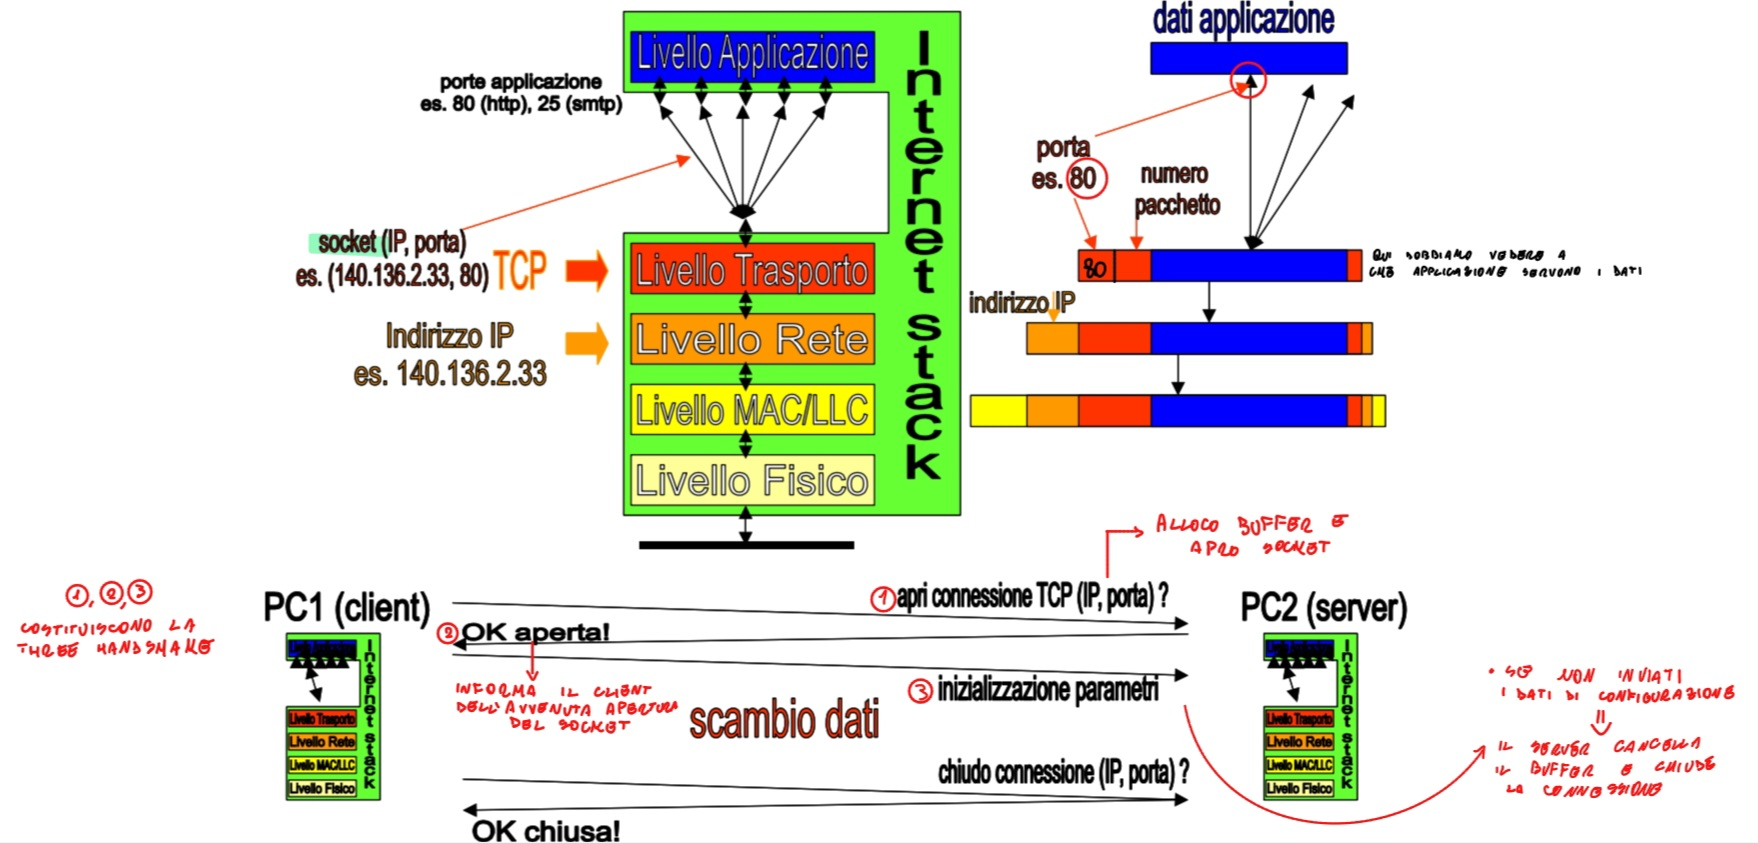
\includegraphics[width=1\linewidth]{foto reti di calcolatori/trasporto_socket.jpg}
    \caption{Apertura di una connessione TCP e concetto di socket tra applicazioni.
Il socket è rappresentato come una linea che collega il livello trasporto (associato all'indirizzo IP sottostante) a una porta specifica di un'applicazione del livello applicazione. 
Si può inoltre osservare che, al livello trasporto, i dati sono incapsulati aggiungendo in testa al pacchetto il numero di porta e il contatore dei segmenti di TCP.}

\end{figure}

\begin{notebox}{Chiusura della connessione}
La connessione TCP viene chiusa con uno scambio \texttt{FIN/ACK} tra client e server, liberando le porte usate e garantendo il completamento di tutti i dati ancora in transito.
\end{notebox}


% ===============================================================
\subsection{Programmazione Socket con UDP e TCP (terza esercitazione)}

I processi applicativi comunicano tra loro inviando messaggi attraverso i \textbf{socket}.

Un \textbf{processo} è un programma in esecuzione su un host. Processi su host diversi comunicano scambiandosi messaggi.

Un \textbf{socket} è un'interfaccia software, analoga a una "porta", che collega il processo applicativo (livello Applicazione) con il protocollo di trasporto sottostante (livello Trasporto, gestito dal Sistema Operativo, come TCP o UDP).


Il programmatore ha il pieno controllo del socket lato applicazione, mentre il lato trasporto è controllato dal Sistema Operativo.
\vspace{0.5cm}


Per identificare un processo ricevente [sia che sia un processo client(il quale inizia la comunicazione) che server(il quale aspetta di essere contattato)], sono necessari due elementi:
\begin{enumerate}
    \item \textbf{Indirizzo IP} dell'host.
    \item \textbf{Numero di porta} associato al processo sull'host.
\end{enumerate}

\vspace{0.5cm}
Esistono due tipologie principali di socket, che rispecchiano i due protocolli di trasporto fondamentali:

\begin{itemize}
    \item \textbf{Socket UDP:} per comunicazioni non affidabili (datagrammi).
    \item \textbf{Socket TCP:} per comunicazioni affidabili e orientate alla connessione (stream di byte).
\end{itemize}

% ------------------------------------------------
\subsubsection{Programmazione Socket con UDP}

UDP è un protocollo \textit{connectionless} (senza connessione). Non esiste una fase preliminare di instaurazione della connessione (handshake) tra client e server.

\begin{defbox}{Caratteristiche Socket UDP}
\begin{itemize}
    \item \textbf{Nessun handshake:} I dati vengono inviati immediatamente senza preavviso.
    \item \textbf{Indirizzamento esplicito:} Il mittente deve allegare l'indirizzo IP e la porta del destinatario a \textbf{ogni singolo pacchetto} (datagramma).
    \item \textbf{Ricezione:} Il ricevente deve estrarre l'indirizzo del mittente dal pacchetto per poter rispondere.
    \item \textbf{Inaffidabilità:} I pacchetti possono arrivare in disordine o andare persi.
\end{itemize}
\end{defbox}

\begin{esempiobox}{Flusso logico Client/Server UDP}
\textbf{Server:}
\begin{enumerate}
    \item Crea il socket UDP.
    \item Lo associa a una porta locale nota (\texttt{bind}).
    \item Entra in un ciclo infinito e attende passivamente i pacchetti (\texttt{recvfrom}).
\end{enumerate}
\textbf{Client:}
\begin{enumerate}
    \item Crea il socket UDP.
    \item Invia il datagramma specificando IP e porta del server (\texttt{sendto}).
    \item Attende l'eventuale risposta.
\end{enumerate}
\end{esempiobox}

\newpage
% ------------------------------------------------
\subsubsection{Programmazione Socket con TCP}

TCP è un protocollo \textit{connection-oriented}. 

Prima di scambiare dati, client e server devono stabilire una connessione tramite un \textit{three-way handshake} (stretta di mano a tre vie).

\begin{defbox}{Caratteristiche Socket TCP}
\begin{itemize}
    \item \textbf{Connessione affidabile:} Garantisce l'arrivo dei dati in ordine e senza errori (byte stream pipe).
    \item \textbf{Handshake:} Il client deve contattare il server per avviare la connessione prima di inviare dati.
    \item \textbf{Stream:} Una volta connessi, non serve specificare l'indirizzo per ogni pacchetto; i dati scorrono nel "tubo" logico stabilito.
\end{itemize}
\end{defbox}

\begin{notebox}{Socket di Benvenuto vs Socket di Connessione}
Una caratteristica fondamentale di TCP è la gestione di socket distinti sul server per gestire più client contemporaneamente:

\begin{itemize}
    \item \textbf{Welcoming Socket (Socket di benvenuto):} È il socket iniziale del server, sempre in ascolto sulla porta pubblica (es. porta 80). Serve \textbf{solo} ad accettare il primo contatto del client.
    \item \textbf{Connection Socket (Socket di connessione):} Quando il server accetta un contatto, crea dinamicamente un \textbf{nuovo socket dedicato} esclusivamente a quel client specifico.
\end{itemize}

Questo meccanismo permette al server di distinguere i client e gestire più conversazioni parallele.
\end{notebox}

\begin{esempiobox}{Flusso logico Client/Server TCP}
\textbf{Server:}
\begin{enumerate}
    \item Crea il \textit{welcoming socket} e lo associa alla porta (\texttt{bind}).
    \item Si mette in ascolto (\texttt{listen}).
    \item Quando arriva una richiesta, usa \texttt{accept()} per generare il \textit{connection socket} dedicato.
    \item Chiude il socket di connessione alla fine della sessione, ma lascia aperto quello di benvenuto.
\end{enumerate}
\textbf{Client:}
\begin{enumerate}
    \item Crea il socket TCP.
    \item Usa \texttt{connect()} specificando IP e porta del server per avviare l'handshake.
    \item Invia e riceve dati (\texttt{send}/\texttt{recv}).
\end{enumerate}
\end{esempiobox}

\newpage
\newpage
\subsection{Multiplexing e Demultiplexing (dei socket TCP e UDP)}

Una delle funzioni cruciali del Livello di Trasporto è permettere a più applicazioni (es. un browser web, un videogioco e un client email) di condividere l'unica connessione di rete fisica del computer. Questo processo si divide in due fasi:
\begin{itemize}[leftmargin=*]
    \item \textbf{Multiplexing (Mittente):} Raccoglie i dati da diversi \textit{socket} (le "porte" delle applicazioni), aggiunge l'header di trasporto (che contiene le porte sorgente e destinazione) e passa tutto al livello di rete sottostante.
    \item \textbf{Demultiplexing (Ricevente):} Legge l'header dei segmenti in arrivo e li consegna al \textit{socket} corretto.
\end{itemize}

Tuttavia, il modo in cui i pacchetti vengono smistati in ricezione cambia radicalmente a seconda del protocollo utilizzato (UDP o TCP).

\subsubsection{Confronto: Demultiplexing UDP vs TCP}

\subsubsection*{1. UDP: Demultiplexing Senza Connessione (Connectionless)}

Nel protocollo UDP, il server non tiene traccia di "chi" ha inviato cosa. Lo smistamento si basa \textbf{esclusivamente sulla porta di destinazione}.

\begin{figure}[H]
    \centering
    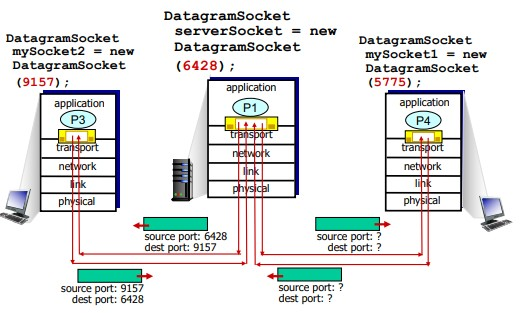
\includegraphics[width=0.8\linewidth]{foto reti di calcolatori/demux_udp.jpg}
    \caption{\textbf{Scenario UDP:} Se due host diversi inviano datagrammi allo stesso server sulla porta 6428, i dati finiranno tutti mescolati all'interno dello stesso singolo \textit{socket} .}
    \label{fig:demux_udp}
\end{figure}

Come si nota nella Figura~\ref{fig:demux_udp}, UDP agisce come una grande "buca delle lettere" condivisa: non importa chi sia il mittente, se il pacchetto ha scritto "Porta 6428", viene buttato in quell'unico contenitore . Questo è molto veloce, ma lascia all'applicazione l'onere di separare i messaggi dei vari client.

\newpage

\subsubsection*{2. TCP: Demultiplexing Orientato alla Connessione (Connection-oriented)}

Nel protocollo TCP, la sicurezza e l'isolamento sono fondamentali. Un \textit{socket} TCP non è identificato solo dalla porta, ma da una \textbf{tupla di 4 parametri}: IP Sorgente, Porta Sorgente, IP Destinazione, Porta Destinazione.

\begin{figure}[H]
    \centering
    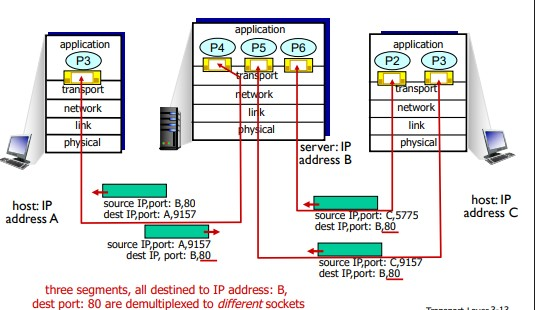
\includegraphics[width=0.8\linewidth]{foto reti di calcolatori/demux_tcp.jpg}
    \caption{\textbf{Scenario TCP:} Tre segmenti arrivano allo stesso server (IP B) sulla stessa porta (80). Il server, leggendo gli indirizzi IP e le porte sorgente, crea e instrada i dati in tre \textit{socket} completamente separati.}
    \label{fig:demux_tcp}
\end{figure}

Come mostrato nella Figura~\ref{fig:demux_tcp}, TCP agisce come un centralino intelligente. Quando un nuovo client si connette alla porta 80 (la porta pubblica del server web), il server genera un nuovo \textit{thread} (processo) e un nuovo \textit{socket} dedicato esclusivamente a quella specifica conversazione. 

\begin{tcolorbox}[colback=blue!5!white, colframe=blue!75!black, title=\textbf{Sintesi per l'esame}]
\begin{itemize}[leftmargin=*]
    \item \textbf{Socket UDP:} Identificato da \textbf{2 parametri} (IP Destinazione, Porta Destinazione). Pacchetti da mittenti diversi finiscono nello stesso socket .
    \item \textbf{Socket TCP:} Identificato da \textbf{4 parametri} (IP e Porta Sorgente + IP e Porta Destinazione). Pacchetti da mittenti diversi vengono rigorosamente instradati in socket separati, garantendo l'isolamento delle sessioni .
\end{itemize}
\end{tcolorbox}



\newpage
\section*{Servizi di Trasporto}
Le applicazioni richiedono diversi servizi al livello di trasporto:
\begin{itemize}
    \item \textbf{Integrità dei dati:} Alcune app (file transfer) non tollerano perdite; altre (audio/video) sì.
    \item \textbf{Timing:} Alcune app (giochi, telefonia) richiedono bassi ritardi.
    \item \textbf{Throughput:} Applicazioni multimediali richiedono una banda minima garantita.
    \item \textbf{Sicurezza:} Crittografia e autenticazione.
\end{itemize}

% ===============================================================
% ===============================================================
\subsubsection{Tabella di confronto: Socket UDP vs TCP}


\begin{table}[H]
    \centering
    \renewcommand{\arraystretch}{1.6} % Aumenta spaziatura righe
    \begin{tabularx}{\textwidth}{@{} >{\bfseries}l X X @{}}
        \toprule
        \textbf{Caratteristica} & \textbf{Socket UDP} & \textbf{Socket TCP} \\
        \midrule
        
        Tipo di Connessione & 
        \textbf{Connectionless} (Senza connessione). Non esiste una fase di handshake: il mittente inizia subito a inviare dati. & 
        \textbf{Connection-oriented} (Orientato alla connessione). Richiede un \textit{handshake} iniziale (3-way) tra client e server. \\
        \addlinespace
        
        Affidabilità & 
        \textbf{Best-effort}. Non garantisce l'arrivo dei dati. I pacchetti possono essere persi, duplicati o arrivare in disordine. & 
        \textbf{Affidabile}. Garantisce che i dati arrivino a destinazione senza errori, senza duplicati e nell'ordine corretto. \\
        \addlinespace
        
        Unità di trasmissione & 
        \textbf{Datagramma}. I messaggi sono pacchetti discreti e indipendenti l'uno dall'altro. I confini del messaggio sono preservati. & 
        \textbf{Byte Stream}. I dati sono visti come un flusso continuo di byte (come un tubo), senza confini di messaggio intrinseci. \\
        \addlinespace
        
        Indirizzamento & 
        L'applicazione deve specificare IP e Porta del destinatario in \textbf{ogni singolo pacchetto} inviato (\texttt{sendto}). & 
        L'indirizzo è definito al momento della connessione (\texttt{connect}). I dati successivi vengono inviati sul canale stabilito. \\
        \addlinespace
        
        Gestione lato Server & 
        Il server utilizza \textbf{un unico socket} per ricevere i datagrammi da tutti i client indistintamente. & 
        Il server usa un socket per l'ascolto (\textit{welcoming}) e crea un \textbf{nuovo socket dedicato} per ogni client connesso. \\
        \addlinespace
        
        Velocità e Overhead & 
        Basso overhead e maggiore velocità (nessun controllo di flusso/congestione). & 
        Overhead maggiore dovuto ai meccanismi di controllo, riordino e conferma (ACK) dei pacchetti. \\
        
        \bottomrule
    \end{tabularx}
    \caption{Differenze tra programmazione Socket UDP e TCP.}
    \label{tab:confronto_socket}
\end{table}


\begin{notebox}{SSL/TLS}
TCP e UDP non offrono cifratura nativa. SSL (Secure Sockets Layer) fornisce crittografia sopra TCP, garantendo sicurezza a livello applicativo.
\end{notebox}

% ===============================================================


\section*{Controllo di Flusso e di Congestione}

TCP funziona tra due dispositivi di una rete, anche molto distanti tra loro, e implementa tecniche di \textbf{controllo di flusso} e \textbf{controllo della congestione} per ridurre il problema della \textbf{latenza di rete elevata} (tempo di andata e ritorno dei pacchetti).

Il problema può essere schematizzato così:

\begin{itemize}
    \item \textbf{Invio di un pacchetto e attesa dell’ACK prima del successivo:}
    \begin{itemize}
        \item Vantaggio: semplice e affidabile.
        \item Svantaggio: \textit{troppo lento}, soprattutto se la latenza è elevata.
    \end{itemize}

    \item \textbf{Invio di tutti i pacchetti consecutivamente senza attesa:}
    \begin{itemize}
        \item Vantaggio: massima velocità teorica.
        \item Svantaggi:
        \begin{itemize}
            \item Possibile congestione dei router intermedi, con conseguente perdita di pacchetti.
            \item Possibile saturazione del destinatario, incapace di gestire il ritmo di arrivo.
        \end{itemize}
    \end{itemize}
\end{itemize}

Per evitare entrambe le estremità (troppo lento / troppo veloce), TCP adotta:

\begin{itemize}
    \item un \textbf{meccanismo di controllo di flusso}, basato sulla finestra scorrevole;
    \item un \textbf{meccanismo di controllo della congestione}, basato sul dimensionamento della finestra scorrevole..
\end{itemize}

L’obiettivo è trovare il \textbf{massimo ritmo di invio sostenibile} dal router più lento del cammino e dal destinatario finale.



% ===============================================================
\subsection{Controllo della congestione}

Il \textbf{controllo della congestione} regola la velocità di invio in base al comportamento della rete e dei router intermedi:

\begin{itemize}
    \item TCP regola dinamicamente la \textbf{SW }.
    \item SCOPO: evitare la saturazione dei router e mantenere la rete stabile ed efficiente, inviando pacchetti al massimo ritmo sostenibile dal router più lento.
\end{itemize}

\begin{figure}[H]
    \centering
    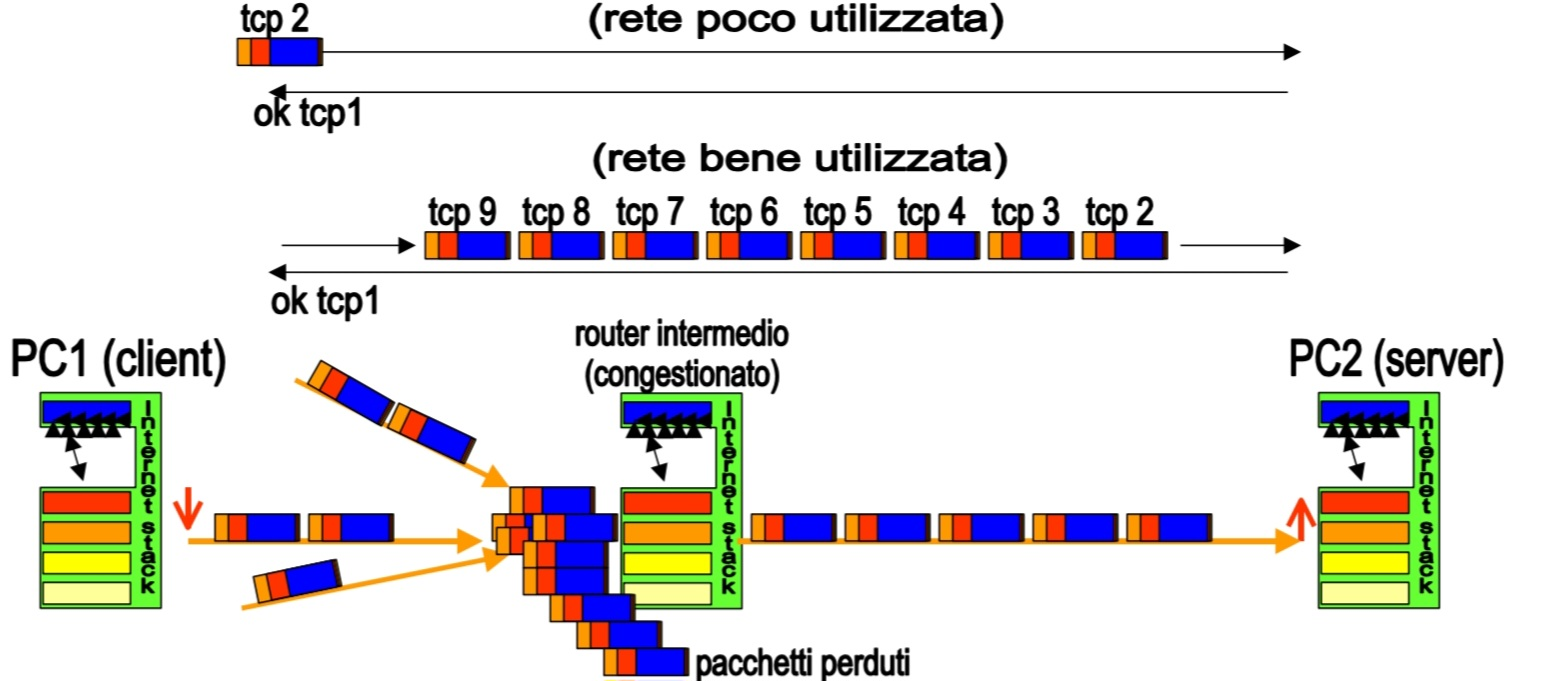
\includegraphics[width=0.9\linewidth]{foto reti di calcolatori/congestione.jpg}
    \caption{Esempio di router intermedio congestionato: più connessioni TCP condividono la stessa risorsa di rete.}
\end{figure}



% ===============================================================
\subsection{Controllo di flusso}

Una forma di congestione può comparire anche sul destinatario finale, nel caso in cui esso non sia in grado di ricevere o elaborare i pacchetti alla velocità con cui il mittente li invia.  
Il \textbf{controllo di flusso} evita la saturazione del buffer di ricezione.

Ogni segmento TCP contiene il campo:

\[
\textbf{RB} = \text{numero massimo di byte che il ricevitore può accettare}
\]

\begin{notebox}{Funzione del controllo di flusso}
Il controllo di flusso garantisce che il \textbf{buffer di ricezione (RB)} non venga saturato, consentendo al destinatario di elaborare i dati al proprio ritmo.  
In pratica, il mittente non può mai inviare più dati di quelli che il destinatario dichiara di poter immagazzinare.

Operativamente, questo si traduce nella condizione:
\[
\text{SW} \leq \text{RB}
\]
cioè la finestra di trasmissione non può superare la capacità del buffer di ricezione.
\end{notebox}



% ===============================================================
\subsection{Sliding Window (Finestra Scorrevole)}

La \textbf{Sliding Window (SW)} è il meccanismo che permette di combinare controllo di flusso e controllo della congestione

\vspace{1cm}
\textbf{Funzionamento della SW:}

La finestra scorrevole \textbf{(SW o numero di finestra)} è un valore intero che indica quanti pacchetti consecutivi possono essere inviati senza attendere conferma.  

Parte tipicamente da 1.

\begin{itemize}
    \item Il mittente può spedire fino a \textbf{SW} pacchetti, poi deve attendere gli ACK.
    \item Se i pacchetti vengono confermati, la finestra può crescere.
    \item Se alcuni pacchetti non ricevono ACK, vengono ritrasmessi e SW viene ridotta.
    \item L’obiettivo è lasciare “in sospeso” non più di SW pacchetti per evitare saturazioni.
\end{itemize}

\begin{figure}[H]
    \centering
    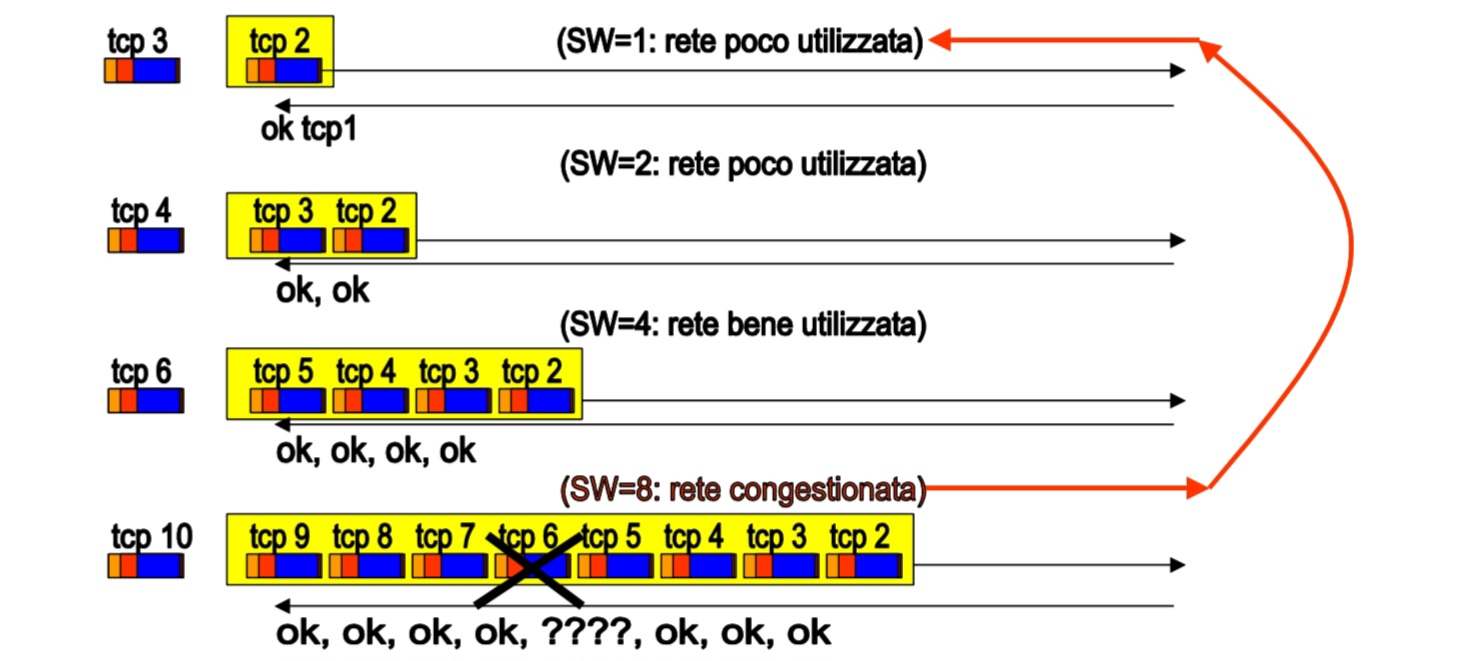
\includegraphics[width=0.9\linewidth]{foto reti di calcolatori/sliding_window.jpg}
    \caption{Evoluzione della Sliding Window: crescita quando i pacchetti sono confermati, riduzione in caso di congestione o perdita.}
\end{figure}


% -------------------------
\begin{esempiobox}{Esempio pratico di Sliding Window}

    SW iniziale = 1 (pacchetto sonda).
    \vspace{1cm}

    \textbf{Controllo di congestione della rete}
\begin{itemize}
    \item \textbf{Slow Start (N = 2N)}: ogni ACK ricevuto raddoppia SW (1 → 2 → 4 → 8 …).  
          Crescita rapida per sondare la capacità della rete.
    \item Se un pacchetto non viene confermato:
    \begin{itemize}
        \item Scade Timeout → SW viene riportata a 1 (segnale di congestione di un router intermedio).
    \end{itemize}
    \item \textbf{Congestion Avoidance (N = N + 1)}: quando SW raggiunge metà della soglia critica precedente, la crescita diventa lineare.  
    
          Aumento cautissimo per evitare di saturare il router (dando modo al router congestionato di smaltire i pacchetti accumulati).
\end{itemize}
\vspace{1cm}
\textbf{Controllo di flusso}

    In parallelo, avviene Controllo di flusso: SW non può superare RB e controlla che non vengano spediti più di SW pacchetti oltre l’ultimo non confermato.
\end{esempiobox}
% -------------------------



\begin{notebox}{Sintesi del meccanismo}
Il meccanismo della Sliding Window permette a TCP di:
\begin{itemize}
    \item Accelerare gradualmente il ritmo di trasmissione.
    \item Ridurre bruscamente la finestra in caso di congestione.
    \item Evitare di saturare il buffer del destinatario.
    \item Adattarsi dinamicamente alle condizioni della rete.
\end{itemize}
\end{notebox}




\begin{notebox}{Indipendenza delle sorgenti TCP}
In una rete reale, le varie connessioni TCP che attraversano lo stesso router 
sono completamente indipendenti e non coordinate tra loro.  
Ogni mittente regola la propria finestra di congestione (\textbf{cwnd}) basandosi 
solo sui feedback della sua connessione.

Conseguenza: mentre una sorgente rileva congestione e riduce SW a 1, altre connessioni potrebbero simultaneamente aumentare la finestra in maniera esponenziale.  
La somma di comportamenti \textbf{non coordinati} mantiene il router vicino alla saturazione, rendendo necessario un meccanismo prudenziale che riporti la finestra a valori molto piccoli quando si rileva congestione.
\end{notebox}

\newpage
\begin{esempiobox}{Esempio grafico di Slow Start e Congestion Avoidance}

La crescita della finestra TCP (\textbf{SW}) durante il controllo della congestione può essere rappresentata così:

\[
\text{Slow Start: crescita esponenziale } (N \leftarrow 2N)
\]

\begin{verbatim}
#
##
####
########
################
################################
###############################################O################
\end{verbatim}

Nel punto segnato con \texttt{O} la finestra ha dimensione 64 e si perde un ACK  
⇒ rilevata congestione.

---

Dopo la perdita:

\[
\text{soglia} = \frac{1}{2} \cdot \text{SW}_{\text{prima della perdita}} = 32
\]

TCP riparte da \textbf{SW= 1} e ricresce fino alla soglia 32, ma una volta raggiunta:

\[
\text{Congestion Avoidance: crescita lineare } (N \leftarrow N+1)
\]

\begin{verbatim}
#
##
####
########
##################
####################################
#####################################
######################################
#######################################
########################################
#########################################
\end{verbatim}

\textbf{Interpretazione:}

\begin{itemize}
    \item Prima della perdita, la crescita è rapida (esponenziale) per “sondare” la rete.
    \item Dopo la perdita, TCP riparte da 1 perché altri client indipendenti potrebbero
          star aumentando a loro volta la velocità.
    \item Superata metà della soglia critica (32), la crescita diventa prudente:
          incremento lineare per evitare nuove congestioni.
\end{itemize}

\end{esempiobox}

% ===============================================================
\subsection{Risoluzione delle perdite: ACK cumulativi e Selective Retransmission}

\begin{figure}[H]
    \centering
    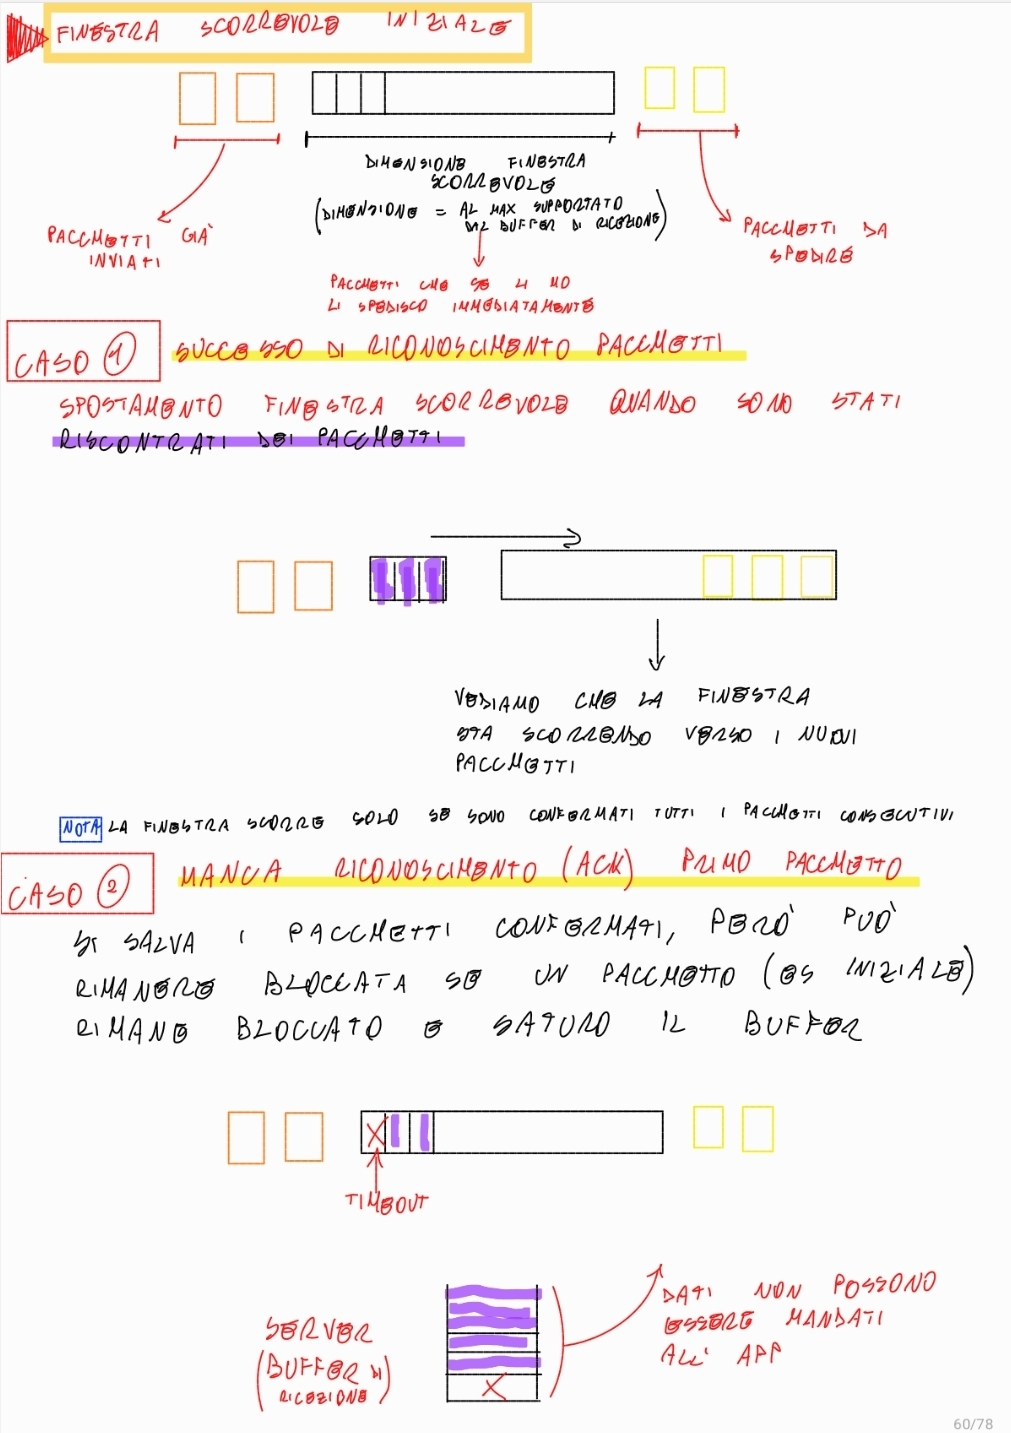
\includegraphics[width=0.8\linewidth]{foto reti di calcolatori/SW.jpg}
    \caption{Comportamenti della SW}
    \label{fig:placeholder}
\end{figure}

La Sliding Window funziona solo se il mittente riceve riscontri dal destinatario sotto forma di ACK.


Quando un pacchetto viene perso, TCP possiede due strategie principali per gestire la ritrasmissione:

\begin{itemize}
    \item \textbf{Cumulative ACK + Ritrasmissione cumulativa}
    \item \textbf{Selective ACK (SACK) + Selective Retransmit}
\end{itemize}

Questi due approcci determinano \emph{quanti} segmenti devono essere ritrasmessi quando si verifica un timeout o una perdita.

% ---------------------------------------------------------------
\subsection*{ACK Cumulativi}

TCP, nella sua versione base, utilizza \textbf{ACK cumulativi}.  
Un ACK cumulativo conferma implicitamente \emph{tutti i segmenti ricevuti correttamente fino al numero indicato}.

Esempio:
\[
\text{ACK = 6} \Rightarrow \text{il destinatario ha ricevuto correttamente i segmenti } 1,2,3,4,5.
\]

Se un segmento è mancante (ad esempio il 3):

\[
1,2,\_,4,5 \Rightarrow \text{ACK = 3}
\]

Il mittente sa che \textbf{3 non è arrivato}.

\begin{defbox}{Ritrasmissione Cumulativa (Go-Back-N)}
Con gli ACK cumulativi, quando scade un timeout relativo al segmento $N$,  
\textbf{il mittente ritrasmette TUTTI i segmenti da $N$ in avanti},  
anche quelli che erano stati ricevuti correttamente ma non ancora riconosciuti cumulativamente.
\[
\text{Timeout sul pacchetto } 3 \Rightarrow \text{ritrasmetto } 3,4,5,6,\ldots
\]
È una strategia semplice ma inefficiente quando la rete perde pochi pacchetti.
\end{defbox}


\vspace{1cm}
% ---------------------------------------------------------------
\subsection*{Selective ACK e Selective Retransmit}

Poiché la ritrasmissione cumulativa può essere inefficiente, TCP introduce un’estensione denominata:

\[
\textbf{SACK (Selective ACKnowledgment)}
\]

Con i SACK, il destinatario può informare il mittente esattamente \textbf{quali segmenti ha ricevuto correttamente} e quali no.

Esempio:
\[
\text{Ricevuti: } 1,2,4,5,6,7 \Rightarrow \text{SACK indica che manca solo il segmento 3}
\]

\begin{defbox}{Selective Retransmit (Selective Repeat)}
Quando un segmento va perso,  
\textbf{TCP ritrasmette esclusivamente il pacchetto mancante},  
senza reinviare tutti quelli successivi.
\[
\text{Timeout su } 3 \Rightarrow \text{ritrasmetto SOLO } 3
\]
Questo approccio riduce il traffico inutile e migliora le prestazioni nelle reti moderne.
\end{defbox}


% ---------------------------------------------------------------
\begin{esempiobox}{Differenza fondamentale tra le due strategie}

Supponiamo che la sorgente abbia inviato i segmenti:
\[
1,2,3,4,5,6
\]
e che il segmento \textbf{3} si perda.

\textbf{Con ACK cumulativi (Go-Back-N):}
\begin{itemize}
    \item Il destinatario invia sempre ACK = 3.
    \item Scade il timeout sul segmento 3.
    \item Il mittente ritrasmette: 3,4,5,6.
\end{itemize}

\textbf{Con Selective ACK (Selective Repeat):}
\begin{itemize}
    \item Il destinatario invia SACK indicando che mancano solo alcuni segmenti.
    \item Il timeout sul segmento 3 provoca la ritrasmissione del solo 3.
    \item Nessun reinvio dei segmenti 4,5,6.
\end{itemize}

\end{esempiobox}

% ---------------------------------------------------------------
\begin{notebox}{Sintesi}
\begin{itemize}
    \item \textbf{ACK cumulativi:} facili da gestire, ma inefficienti in caso di perdite isolate.  
          Ritrasmettono tutti i segmenti dalla perdita in avanti.
    \item \textbf{Selective ACK:} permettono ritrasmissioni mirate → maggiore efficienza e minor traffico.
\end{itemize}
\end{notebox}

\newpage
% ===============================================================






\newpage
% ===============================================================
\section{Livello Applicazione (5)}

\begin{figure}[H]
    \centering
    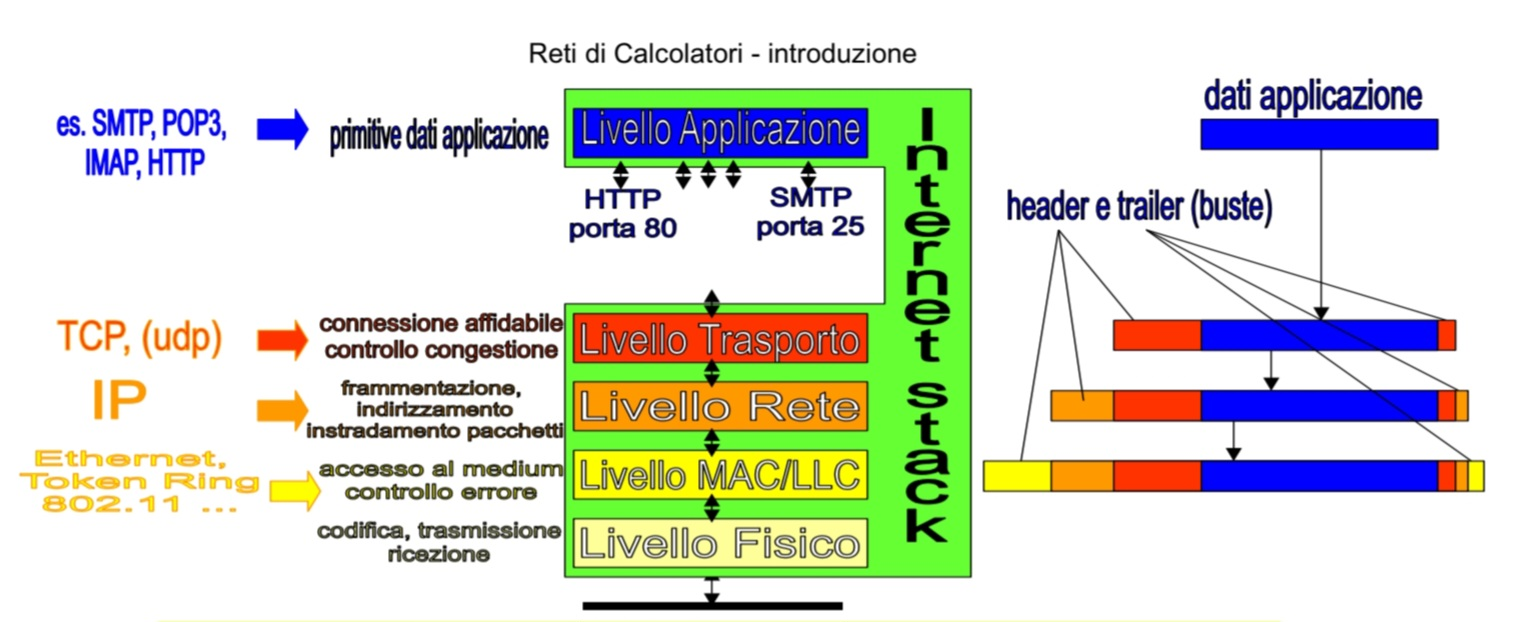
\includegraphics[width=0.8\linewidth]{foto reti di calcolatori/Applicazione.jpg}
    \label{fig:placeholder}
\end{figure}
Il \textbf{livello Applicazione} è il livello più alto del modello Internet.
Qui risiedono i protocolli che forniscono servizi direttamente alle applicazioni
con le quali interagiscono gli utenti (browser, posta elettronica, DNS, streaming, ecc.).

A differenza dei livelli inferiori, il livello Applicazione non gestisce pacchetti o segmenti:
\textbf{gestisce dati significativi per l’utente} e utilizza i servizi dei livelli
Trasporto e Rete per comunicare.

% ===============================================================
\subsection{Ruolo del Livello Applicazione}

Il livello Applicazione fornisce:
\begin{itemize}
    \item servizi di rete per applicazioni utente (web, email, file sharing, ecc.);
    \item protocolli standard che definiscono il formato e la semantica dei messaggi;
    \item interfacce tra software applicativi e stack TCP/IP.
\end{itemize}

Ogni applicazione sceglie se utilizzare \textbf{TCP} o \textbf{UDP} in base alle
proprie esigenze:
\begin{itemize}
    \item applicazioni che richiedono affidabilità → \textbf{TCP};
    \item applicazioni time-sensitive → \textbf{UDP}.
\end{itemize}

\begin{notebox}{Applicazioni che usano TCP e UDP}
\textbf{TCP}: HTTP, HTTPS, FTP, SMTP, IMAP, SSH  


\textbf{UDP}: DNS (la maggior parte delle richieste), VoIP, streaming, gaming
\end{notebox}

% ===============================================================
\subsection{Protocolli principali del Livello Applicazione}

Il livello Applicazione comprende numerosi protocolli. Tra i principali:

\begin{itemize}
    \item \textbf{DNS} — risoluzione dei nomi in indirizzi IP;
    \item \textbf{HTTP/HTTPS} — trasferimento di pagine web;
    \item \textbf{SMTP, POP3, IMAP} — posta elettronica (spedizione e trasporto messaggi / leggere messaggi);
    \item \textbf{FTP/SFTP} — trasferimento file;
    \item \textbf{DHCP} — assegnazione dinamica degli indirizzi IP;
    \item \textbf{SSH} — gestione remota sicura;
    \item \textbf{NTP} — sincronizzazione dell’orario nelle reti.
\end{itemize}

Nei paragrafi seguenti vengono presentati i più importanti e argomenti correlati al loro funzionamento.

\newpage
% ===============================================================

\subsection{Servizio DNS e Nomi di Dominio}

Il \textbf{Domain Name System (DNS)} è un servizio fondamentale dell’architettura di rete
che permette di tradurre i nomi simbolici usati dagli utenti (come \texttt{www.unibo.it})
negli indirizzi IP numerici richiesti dal livello Rete e dai router.

A differenza degli indirizzi IP, difficili da ricordare, i nomi di dominio sono
mnemonici, gerarchici e facilmente interpretabili.

\begin{defbox}{DNS -- Domain Name System}
Il \textbf{DNS} è un sistema distribuito e gerarchico che associa un
\[
\text{nome di dominio} \quad \longrightarrow \quad \text{indirizzo IP}
\]
utilizzando una rete globale di server DNS posti a livelli successivi.
Ogni host della rete deve conoscere almeno un DNS server locale
per inviare richieste di risoluzione dei nomi.
\end{defbox}
%===================================================


\subsection*{Servizi offerti dal DNS}

Oltre alla traduzione da hostname a indirizzo IP, il DNS offre altri servizi critici:

\begin{itemize}
    \item \textbf{Host Aliasing:} permette di avere alias mnemonici (es. \texttt{www.ibm.com}) per nomi canonici complessi (es. \texttt{servereast.backup2.ibm.com}).
    \item \textbf{Mail Server Aliasing:} permette di avere indirizzi email semplici (es. \texttt{@hotmail.com}) anche se il server di posta ha un nome canonico complesso.
    \item \textbf{Load Distribution:} per siti molto trafficati (es. CNN), a un singolo nome canonico vengono associati \textbf{più indirizzi IP}. Il DNS restituisce l'intera lista ruotando l'ordine, permettendo di distribuire il carico tra server replicati.
\end{itemize}

\begin{notebox}{Perché un database distribuito?}
Perché non usare un singolo server centrale per tutto Internet? Perché \textbf{non scala} ("doesn't scale").
Un server centralizzato avrebbe:
\begin{itemize}
    \item Un singolo punto di guasto (Single Point of Failure).
    \item Volumi di traffico ingestibili.
    \item Distanza elevata dalla maggior parte degli utenti (ritardi).
    \item Difficoltà di manutenzione e aggiornamento del database.
\end{itemize}
\end{notebox}

% ===============================================================
\subsection*{Perché serve il DNS}

Gli utenti e le applicazioni preferiscono utilizzare nomi simbolici:

\begin{itemize}
    \item più intuitivi rispetto a indirizzi IP numerici;
    \item flessibili e descrittivi (es. \texttt{www.informatica.unibo.it});
    \item indipendenti dalla topologia di rete.
\end{itemize}

\begin{notebox}{Problema}
I protocolli di rete e i router operano esclusivamente con \textbf{indirizzi IP}.
Serve quindi un servizio che traduca i nomi simbolici in indirizzi IP validi.
\end{notebox}

\newpage
% ===============================================================
\subsection*{Struttura dei nomi di dominio}

I nomi di dominio hanno una struttura gerarchica a livelli:

\[
\text{host.sottodominio.sottodominio.dominioTLD}
\]

Esempio:  
\[
\texttt{www.informatica.unibo.it}
\]

\begin{itemize}
    \item \texttt{www} → nome dell’host (risorsa);
    \item \texttt{informatica} → sottodominio;
    \item \texttt{unibo} → dominio di secondo livello;
    \item \texttt{it} → Top-Level Domain (TLD).
\end{itemize}

Il dominio radice (root) esiste ma non viene mai scritto esplicitamente.

\begin{notebox}{Univocità dei nomi}
All’interno di uno stesso dominio non possono esistere due risorse con lo stesso nome.
È possibile invece avere nomi uguali in domini diversi
(es. \texttt{pippo@topolinia.it} e \texttt{pippo@paperopoli.com}).
\end{notebox}

% ===============================================================

\subsubsection{Gerarchia dei server DNS}

Il DNS è organizzato come un grande albero di server distribuiti:
\begin{figure}[H]
    \centering
    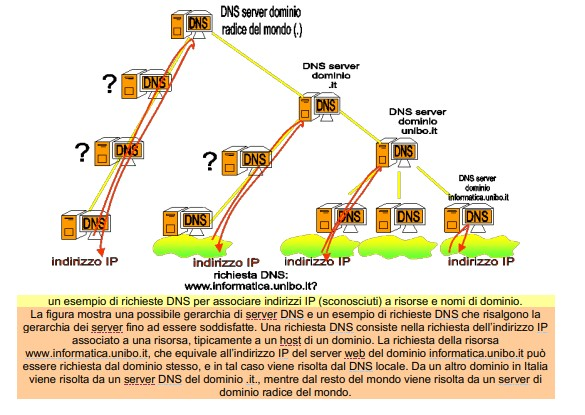
\includegraphics[width=0.8\linewidth]{foto reti di calcolatori/DNS.jpg}
    \caption{}
    \label{fig:placeholder}
\end{figure}

\begin{itemize}
    \item \textbf{Root DNS Servers:} Il livello più alto. Esistono 13 server logici mondiali (etichettati da A a M), ma sono replicati fisicamente in molte copie. Vengono contattati quando il server locale non sa risolvere il nome.
    \item \textbf{Top-Level Domain (TLD) Servers:} Gestiscono i domini di primo livello generici come \texttt{.com}, \texttt{.org}, \texttt{.net} e i domini nazionali come \texttt{.it}, \texttt{.uk}, \texttt{.jp}. Esempi: Verisign gestisce \texttt{.com}, Educause gestisce \texttt{.edu}.
    \item \textbf{Authoritative DNS Servers:} Server dell'organizzazione (o del provider) che forniscono la mappatura definitiva hostname-IP per i propri host (es. il server DNS dell'Università di Bologna).
    \item \textbf{Local DNS Server (Default Name Server):} Non appartiene strettamente alla gerarchia, ma è centrale per il funzionamento. Solitamente fornito dall'ISP o dall'azienda. Agisce come \textbf{proxy}, inoltrando le richieste nella gerarchia per conto dell'host.
\end{itemize}

\begin{esempiobox}{Google Public DNS}
Oltre ai DNS forniti dagli ISP, esistono servizi pubblici come Google DNS (\texttt{8.8.8.8}). Funzionano come resolver veloci e sicuri, offrendo un'alternativa ai DNS locali standard.
\end{esempiobox}

% ===============================================================
\subsection*{Funzionamento di una richiesta DNS}

Quando un host desidera contattare un servizio, ad esempio:

\[
\texttt{www.informatica.unibo.it}
\]

invia una richiesta DNS seguendo questi passaggi:

\begin{enumerate}
    \item L’host invia la richiesta al \textbf{DNS locale} tramite pacchetto UDP.
    \item Se il DNS locale conosce l’indirizzo → risponde subito (cache).
    \item Altrimenti inoltra la richiesta verso livelli sempre più alti:
    \begin{itemize}
        \item server autoritativi del dominio \texttt{unibo.it};
        \item server DNS TLD \texttt{.it};
        \item eventualmente i server DNS root.
    \end{itemize}
    \item Una volta trovato l’indirizzo IP, la risposta ritorna indietro fino all’host richiedente.
\end{enumerate}

\begin{esempiobox}{}
La richiesta per \texttt{www.informatica.unibo.it} segue un percorso diverso a seconda dell’origine:
\begin{itemize}
    \item Se proviene da un host dell’Università di Bologna → risolta dal DNS locale.
    \item Da un altro dominio italiano → risolta da un DNS del dominio \texttt{.it}.
    \item Dal resto del mondo → può richiedere la consultazione dei DNS root.
\end{itemize}
\end{esempiobox}

\begin{notebox}{Risoluzione DNS: iterativa, non ricorsiva}
Sebbene a livello teorico si parli spesso di risoluzione ``ricorsiva'',  
i server DNS \textbf{non eseguono realmente una ricerca ricorsiva completa}.  

Per evitare di sovraccaricare i DNS di livello superiore, la risoluzione è 
\textbf{prevalentemente iterativa}:

\begin{itemize}
    \item Il DNS locale interroga un server superiore.
    \item Se il server superiore non conosce la risposta, \textbf{rimanda al client}  
          l’indirizzo di un server ancora più in alto.
    \item Sarà il \textbf{client DNS} (resolver) a continuare le interrogazioni successive.
\end{itemize}

Questo comportamento impedisce che i server DNS si riempiano di richieste ricorsive
e distribuisce il carico tra client e server.
\end{notebox}


% ===============================================================
\subsection*{Caratteristiche principali del servizio DNS}

\begin{itemize}
    \item Sistema distribuito, scalabile e tollerante ai guasti.
    \item Uso massiccio della cache per ridurre il traffico DNS.
    \item Utilizza principalmente \textbf{UDP porta 53} (richieste brevi e veloci).
    \item Utilizza \textbf{TCP porta 53} per trasferimenti di zone e risposte lunghe.
\end{itemize}

\begin{notebox}{Importanza del DNS}
Il DNS è indispensabile per il funzionamento di:
\begin{itemize}
    \item Web (HTTP/HTTPS),
    \item posta elettronica (SMTP),
    \item servizi cloud e distribuiti,
    \item qualsiasi applicazione che usi nomi simbolici.
\end{itemize}
\end{notebox}


\begin{notebox}{Problema di sicurezza: DNS Man-in-the-Middle}
Il DNS, nella sua forma classica, \textbf{non offre autenticazione} delle risposte.
Un attaccante sulla rete (ad esempio in una Wi-Fi pubblica) può:

\begin{itemize}
    \item intercettare la richiesta DNS del client;
    \item inviare una risposta falsa più veloce di quella del DNS legittimo;
    \item fornire un indirizzo IP controllato dall’attaccante.
\end{itemize}

Questo attacco è noto come \textbf{DNS Man-in-the-Middle} o \textbf{DNS Spoofing}.

Conseguenze:
\begin{itemize}
    \item reindirizzamento verso siti falsi (phishing),
    \item intercettazione del traffico,
    \item installazione di malware.
\end{itemize}

\end{notebox}



\subsection*{DNS Caching}

Il caching è vitale per le prestazioni. Una volta che un server apprende una mappatura, la memorizza nella cache locale.
\begin{itemize}
    \item Le voci vengono eliminate dopo un tempo di vita detto \textbf{TTL (Time To Live)}.
    \item I TLD server sono spesso in cache nei DNS locali, quindi i Root server vengono contattati raramente.
\end{itemize}

\newpage
% ===============================================================
\subsection*{I Record DNS (Resource Records)}

Il database DNS memorizza le informazioni sotto forma di Resource Records (RR).
Il formato generico è: \texttt{(Name, Value, Type, TTL)}.
Il significato di \texttt{Name} e \texttt{Value} dipende dal campo \texttt{Type}:

\begin{table}[H]
\centering
\begin{tabularx}{\textwidth}{l X X}
\toprule
\textbf{Type} & \textbf{Significato (Name $\to$ Value)} & \textbf{Esempio/Note} \\
\midrule
\textbf{A} & \textbf{Hostname $\to$ Indirizzo IP} & Associa un nome standard (es. relay1.bar.foo.com) al suo indirizzo IP (145.37.93.126). \\
\midrule
\textbf{NS} & \textbf{Dominio $\to$ Hostname Server Autorevole} & Indica quale server DNS è autoritativo per un dominio (es. foo.com $\to$ dns.foo.com). \\
\midrule
\textbf{CNAME} & \textbf{Alias $\to$ Nome Canonico} & Associa un alias (es. www.ibm.com) al vero nome canonico (servereast.backup2.ibm.com). \\
\midrule
\textbf{MX} & \textbf{Dominio $\to$ Mail Server} & Specifica il server di posta associato a un nome di dominio (permette di avere mail server e web server sullo stesso nome ma macchine diverse). \\
\bottomrule
\end{tabularx}
\caption{Principali tipi di record DNS}
\end{table}

\begin{esempiobox}{ Configurazione DNS di "Network Utopia"}
    Immaginiamo di aver appena registrato il dominio per una nuova startup chiamata \textbf{Network Utopia} (\texttt{networkutopia.com}). Ecco come utilizziamo i diversi tipi di record per far funzionare i servizi:

    \begin{itemize}
        \item \textbf{Record A (Address) -- "Dove si trova il sito web?"} \\
        Vogliamo che gli utenti raggiungano il nostro sito web. Creiamo un record che collega il nome all'indirizzo IP fisico del server:
        \[ (\texttt{www.networkutopia.com}, \texttt{212.212.212.1}, \textbf{A}) \]
        \textit{Traduzione:} "Il server web si trova all'indirizzo IP 212.212.212.1".

        \item \textbf{Record NS (Name Server) -- "Chi gestisce la mappa?"} \\
        Il sistema DNS mondiale deve sapere a chi chiedere informazioni su di noi. Inseriamo questo record nel server TLD (gestore dei .com):
        \[ (\texttt{networkutopia.com}, \texttt{dns1.networkutopia.com}, \textbf{NS}) \]
        \textit{Traduzione:} "Se cerchi qualsiasi indirizzo dentro questo dominio, chiedi al server dns1".

        \item \textbf{Record MX (Mail Exchange) -- "Dove consegno la posta?"} \\
        Se qualcuno invia una mail a \texttt{supporto@networkutopia.com}, il server mittente deve sapere che non deve contattare il server web, ma quello di posta:
        \[ (\texttt{networkutopia.com}, \texttt{mail.google.com}, \textbf{MX}) \]
        \textit{Traduzione:} "Tutta la posta indirizzata a @networkutopia.com deve essere consegnata ai server di Gmail (o altro provider)".

        \item \textbf{Record CNAME (Canonical Name) -- "Il soprannome"} \\
        Vogliamo che il sito sia raggiungibile anche scrivendo \texttt{home.networkutopia.com}, ma non vogliamo gestire due indirizzi IP diversi. Creiamo un alias:
        \[ (\texttt{home.networkutopia.com}, \texttt{www.networkutopia.com}, \textbf{CNAME}) \]
        \textit{Traduzione:} "Home è solo un altro nome per www. Se cerchi Home, vai dove va www".
    \end{itemize}
\end{esempiobox}
% ===============================================================
\subsection*{Formato dei Messaggi DNS}

Il protocollo DNS utilizza un formato unificato e molto efficiente: i messaggi di interrogazione (\textit{Query}) e quelli di risposta (\textit{Reply}) condividono la stessa identica struttura.

\begin{figure}[H]
    \centering
    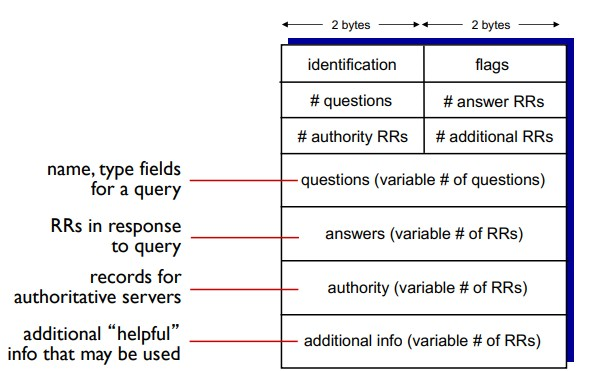
\includegraphics[width=0.7\linewidth]{foto reti di calcolatori/protocolli_messaggi.jpg}
    \caption{Struttura generale di un messaggio DNS. L'intestazione (Header) è fissa a 12 byte, seguita da 4 sezioni a lunghezza variabile nel corpo del messaggio.}
    \label{fig:dns_message_format}
\end{figure}

Come mostrato nella Figura~\ref{fig:dns_message_format}, il messaggio è suddiviso in due macro-sezioni: l'\textbf{Header} e il \textbf{Corpo}.

\vspace{0.3cm}
\textbf{1. L'Intestazione (Header - 12 byte fisse):} \\
Comprende le prime tre righe dello schema (formate da 6 campi da 2 byte, ovvero 16 bit ciascuno):
\begin{itemize}[leftmargin=*]
    \item \textbf{Identification (16 bit):} Un numero identificativo univoco generato dal client. È fondamentale per abbinare in modo corretto e inequivocabile la risposta in arrivo alla specifica richiesta inviata.
    \item \textbf{Flags (16 bit):} Campi di controllo. I bit più importanti indicano:
    \begin{itemize}
        \item \textbf{Query/Reply:} \texttt{0} se il messaggio è un'interrogazione, \texttt{1} se è una risposta.
        \item \textbf{Authoritative:} Impostato a \texttt{1} se il server che risponde è quello \textit{autoritativo} (ufficiale) per il nome richiesto.
        \item \textbf{Recursion Desired:} Impostato dal client se desidera che il server esegua una query ricorsiva al suo posto.
        \item \textbf{Recursion Available:} Impostato dal server per confermare al client che supporta la modalità ricorsiva.
    \end{itemize}
    \item \textbf{Contatori (4 campi da 16 bit):} Indicano il numero esatto di elementi (Resource Record) presenti in ciascuna delle quattro sezioni successive (\# questions, \# answer RRs, \# authority RRs, \# additional RRs).
\end{itemize}

\vspace{0.3cm}
\textbf{2. Il Corpo del messaggio (Lunghezza variabile):}
\begin{itemize}[leftmargin=*]
    \item \textbf{Questions:} Contiene i dettagli della domanda vera e propria (solitamente il nome di dominio da tradurre, es. \texttt{www.unibo.it}, e il tipo di record richiesto, es. Tipo A).
    \item \textbf{Answers:} Contiene i Resource Record (RR) di risposta alla query (es. l'indirizzo IP trovato). In un messaggio di sola query inoltrato dal client, questa sezione è vuota.
    \item \textbf{Authority:} Contiene i record che puntano ai server DNS autoritativi per quel dominio specifico.
    \item \textbf{Additional Info:} Contiene informazioni aggiuntive "di aiuto" (\textit{helpful info}) che non sono state esplicitamente richieste, ma che il server sa che potrebbero tornare utili al client (ad esempio, l'indirizzo IP del server autoritativo appena nominato nella sezione Authority, risparmiando così al client un'ulteriore query per andarlo a cercare).
\end{itemize}



% ===============================================================
\subsection*{Sicurezza del DNS}

Il DNS è vulnerabile a diversi tipi di attacchi informatici:

\begin{enumerate}
    \item \textbf{DDoS Attacks (Distributed Denial of Service):}
    \begin{itemize}
        \item \textit{Contro i Root Servers:} Tentativo di bloccare l'intero internet bombardando i root server. Finora poco efficace grazie al caching locale e al filtraggio del traffico.
        \item \textit{Contro i TLD Servers:} Potenzialmente più pericoloso.
    \end{itemize}
    
    \item \textbf{Redirect Attacks (Man-in-the-Middle / Poisoning):}
    \begin{itemize}
    \item Intercettazione delle query per alterare la risposta.
        \item \textbf{DNS Poisoning:} L'attaccante invia risposte false a un server DNS affinché le memorizzi nella cache (avvelenamento), reindirizzando gli utenti ignari verso siti fraudolenti (phishing).
        
    \end{itemize}
    
    \item \textbf{Exploit per DDoS (DNS Amplification):}
    Gli attaccanti inviano query DNS con l'indirizzo IP sorgente falsificato (spoofed), inserendo l'IP della vittima. Poiché la risposta del server DNS è molto più grande della richiesta (amplificazione), la vittima viene inondata di traffico non richiesto.
\end{enumerate}

\begin{notebox}{DNSSEC}
Per mitigare questi problemi è stato introdotto \textbf{DNSSEC}, un'estensione di sicurezza che aggiunge firme crittografiche ai record DNS per garantirne l'autenticità e l'integrità.
\end{notebox}

\newpage
% ===============================================================
\subsection{HTTP e HTTPS}


Una pagina web è composta da oggetti (HTML, JPEG, Applet, etc.), ognuno indirizzabile tramite un URL.

Il \textbf{HyperText Transfer Protocol} è il protocollo del Web.

\begin{itemize}
    \item \textbf{HTTP}: comunicazione in chiaro su TCP (porta 80).
    \item \textbf{HTTPS}: versione cifrata tramite TLS su TCP (porta 443).
\end{itemize}

\begin{defbox}{Funzionamento di HTTP}
HTTP è stateless: ogni richiesta è indipendente (il server non mantiene informazioni sulle richieste
passate del client).  
Il browser invia richieste \texttt{GET}, \texttt{POST}, \texttt{HEAD}, …  
Il server risponde con codice di stato (200, 404, 500, …) e la risorsa richiesta.
\end{defbox}




\begin{notebox}{Approfondimento: HTTP Persistente vs Non-persistente}
    La differenza fondamentale risiede nella gestione della connessione TCP sottostante:

    \begin{itemize}
        \item \textbf{HTTP Non-persistente:} 
        \begin{itemize}
            \item Viene inviato \textbf{al massimo un oggetto} per connessione TCP, che viene chiusa subito dopo.
            \item Per scaricare una pagina con più oggetti (es. immagini), sono necessarie connessioni multiple (spesso parallele).
            \item \textbf{Svantaggio:} Richiede \textbf{2 RTT} \colorbox{red}{per oggetto} (uno per avviare la connessione TCP (Three-way-handshake), uno per la richiesta HTTP) più il tempo di trasmissione, creando overhead per il sistema operativo .
        \end{itemize}
        
        \item \textbf{HTTP Persistente:}
        \begin{itemize}
            \item Il server lascia la connessione \textbf{aperta} dopo aver inviato la risposta.
        \item Gli oggetti successivi vengono inviati sulla stessa connessione aperta tra client e server.
            \item \textbf{Vantaggio:} Riduce il ritardo a circa \textbf{un solo RTT} per tutti gli oggetti referenziati (in quanto Three-way-handshake si fa solo una volta).
        \end{itemize}
    \end{itemize}
\end{notebox}

\begin{figure}[H]
    \centering
    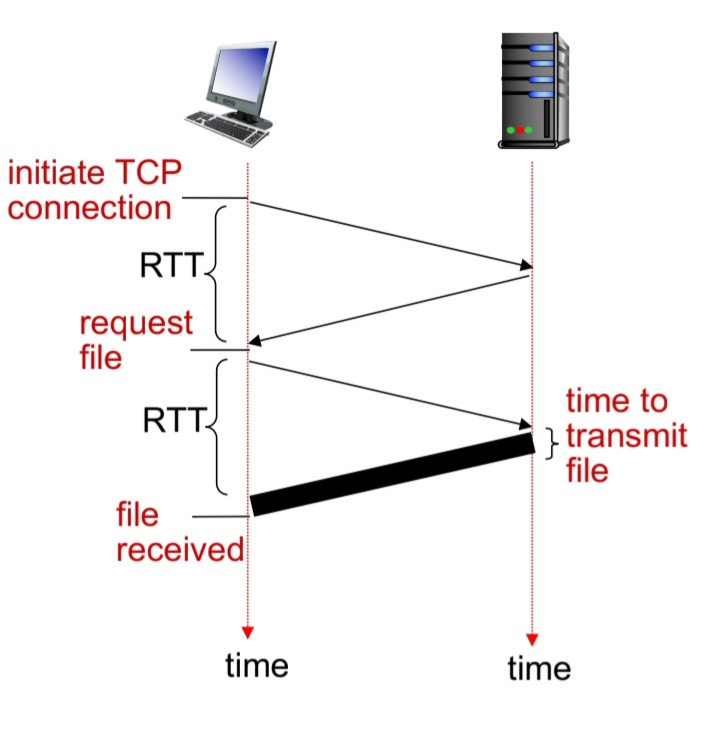
\includegraphics[width=0.4\linewidth]{foto reti di calcolatori/HTTP_RTT.jpg}
    \caption{HTTP non persistente : tempo di risposta}
    \label{fig:placeholder}
\end{figure}




\begin{esempiobox}{Esercizio: Calcolo Tempo di Caricamento (HTTP Persistente vs Non-Persistente)}
    \textbf{Dati del problema:}
    \begin{itemize}
        \item \textbf{Obiettivo:} Calcolare il tempo totale ($T$) per caricare una pagina web.
        \item \textbf{Contenuto:} 1 file HTML base (size 1kb) + 10 immagini (size 10 Mbit ciascuna).
        \item \textbf{Velocità di scaricamento (Bandwidth):} 80 Mbit/s. 
        
        Questo è stato ottenuto tramite lo speedTest ed indica la velocità media di risposta da parte del server per ogni richiesta
        \item \textbf{Parametri di rete:} $RTT_{\text{medio}}$ (Round Trip Time).

        Questo invece è stato calcolato tramite il ping 
    \end{itemize}

    \vspace{0.5cm}
    \textbf{Concetto Chiave (Diagramma Temporale):}
    Per scaricare un oggetto via HTTP su una nuova connessione TCP, sono necessari \textbf{2 RTT} iniziali prima di ricevere i dati:
    \begin{enumerate}
        \item \textbf{1 RTT} per il TCP Handshake (apertura connessione).
        \item \textbf{1 RTT} per inviare la richiesta HTTP GET e ricevere il primo byte di risposta.
    \end{enumerate}
    A questo si aggiunge il \textbf{tempo di trasmissione} ($\Delta F$), calcolato come $\frac{\text{Dimensione}}{\text{Velocità}}$.

    \hrulefill

    \subsubsection*{1. Caso HTTP Non-Persistente}
    In questa modalità, per ogni singolo oggetto (HTML e le 10 immagini) viene aperta e chiusa una nuova connessione TCP. Quindi paghiamo il costo di "apertura" ($2 \times RTT$) per ogni elemento.

    \[
    T_{\text{non-pers}} = \underbrace{\left( 1 \times 2 \cdot $RTT_{\text{medio}}$) \right)}_{\text{File HTML}} + \underbrace{10 \times \left( 2 \cdot RTT_{medio}
    + \frac{10 \text{ Mbit}}{80 \text{ Mbit/s}} \right)}_{\text{10 Immagini}}
    \]
    
    \textbf{Nota:} Il tempo di trasmissione del file HTML (1kb) è considerato trascurabile rispetto agli RTT, quindi appare solo come $2 \cdot RTT$. Per le immagini, invece, calcoliamo $\Delta F = \frac{10}{80} = 0.125$ secondi.

    \hrulefill

    \subsubsection*{2. Caso HTTP Persistente}
    In modalità persistente, il server lascia aperta la connessione TCP dopo aver inviato la risposta. 
    \begin{itemize}
        \item Il \textbf{primo oggetto} (HTML) paga il costo pieno (Handshake + Request = 2 RTT).
        \item Gli \textbf{oggetti successivi} (Immagini) riutilizzano la connessione esistente, risparmiando il tempo di Handshake. Serve solo 1 RTT per la richiesta.
    \end{itemize}

    il moltiplicatore dell'RTT per le immagini scende da 2 a 1:

    \[
    T_{\text{pers}} = \underbrace{\left( 1 \times 2 \cdot RTT_{medio} \right)}_{\text{File HTML (apre la connessione)}} + \underbrace{10 \times \left( \mathbf{1} \cdot RTT_{medio} + \frac{10 \text{ Mbit}}{80 \text{ Mbit/s}} \right)}_{\text{10 Immagini (riutilizzano la connessione)}}
    \]

    \textbf{Risultato:} L'utilizzo di HTTP persistente risparmia $10 \times RTT$ totali rispetto al caso non-persistente.
\end{esempiobox}



\newpage
\subsection*{Messaggi HTTP}

Esistono due tipi di messaggi HTTP: messaggi di \textbf{richiesta} (inviati dal client al server) e messaggi di \textbf{risposta} (inviati dal server al client). Entrambi utilizzano un formato ASCII leggibile dall'uomo.

\subsubsection{Messaggio di Richiesta HTTP}

\begin{figure}[H]
    \centering
    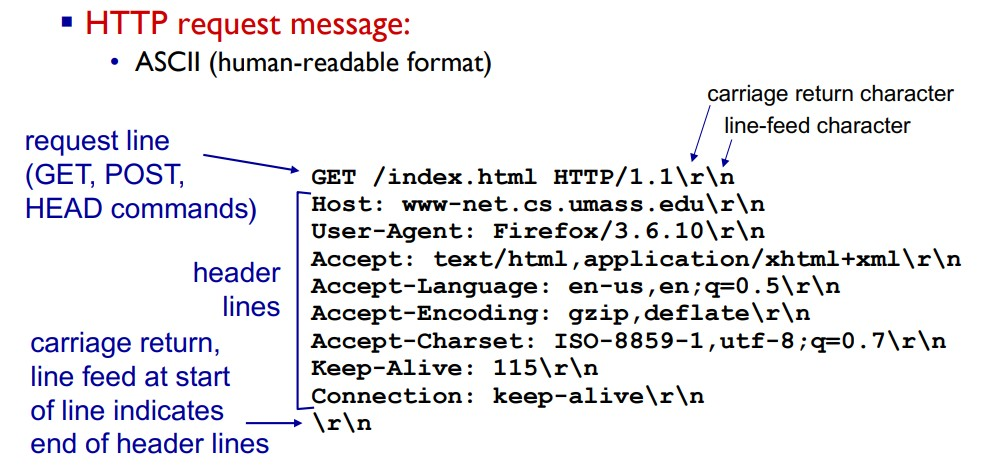
\includegraphics[width=0.5\linewidth]{slide_27.jpg}
    \caption{HTTP request message}
    \label{fig:placeholder}
\end{figure}
Un messaggio di richiesta è composto da quattro parti principali: la \textit{request line}, le \textit{header lines}, una linea vuota e l'\textit{entity body}.

\begin{enumerate}
    \item \textbf{Request Line:} La prima linea del messaggio. Contiene tre campi:
    \begin{itemize}
        \item Il \textbf{metodo} (es. GET, POST, HEAD).
        \item L'\textbf{URL} (il percorso dell'oggetto richiesto).
        \item La \textbf{versione} del protocollo HTTP (es. HTTP/1.1).
    \end{itemize}
    
    \item \textbf{Header Lines:} Linee successive che forniscono informazioni aggiuntive.
    \begin{itemize}
        \item \texttt{Host:} Specifica l'host a cui è rivolta la richiesta (obbligatorio in HTTP/1.1).
        \item \texttt{User-Agent:} Identifica il tipo di browser/client.
        \item \texttt{Connection:} Può specificare \texttt{keep-alive} per richiedere una connessione persistente.
    \end{itemize}
    
    \item \textbf{Linea Vuota:} Una sequenza di Carriage Return e Line Feed (\texttt{\textbackslash r\textbackslash n}) che indica la fine degli header.
    
    \item \textbf{Entity Body:} Il corpo del messaggio. È vuoto nel metodo GET, ma viene utilizzato nel metodo POST per inviare dati al server (es. input di un form).
\end{enumerate}

\begin{notebox}{Invio di Input al Server: GET vs POST}
    Le pagine web spesso includono form per l'input dell'utente. Il modo in cui questi dati vengono inviati dipende dal metodo:
    \begin{itemize}
        \item \textbf{Metodo POST:} L'input viene caricato e inviato all'interno dell'\textbf{entity body} del messaggio di richiesta.
        \item \textbf{Metodo URL (GET):} L'input non è nel corpo, ma viene accodato direttamente nell'\textbf{URL} della request line (es. \texttt{www.sito.com/cerca?q=scimmie\&frutta=banana}).
    \end{itemize}
\end{notebox}

\newpage
\subsubsection{Tipi di Metodi HTTP}
I metodi definiscono l'azione richiesta al server.
\begin{itemize}
    \item \textbf{HTTP/1.0:} Supportava principalmente \texttt{GET}, \texttt{POST} e \texttt{HEAD} (simile alla GET ma il server risponde senza inviare l'oggetto richiesto, utile per debug o cache).
    \item \textbf{HTTP/1.1:} Ha introdotto nuovi metodi:
    \begin{itemize}
        \item \texttt{PUT}: Carica un file nel percorso specificato nell'URL (upload).
        \item \texttt{DELETE}: Cancella il file specificato nell'URL.
    \end{itemize}
\end{itemize}

\subsubsection{Messaggio di Risposta HTTP}

\begin{figure}[H]
    \centering
    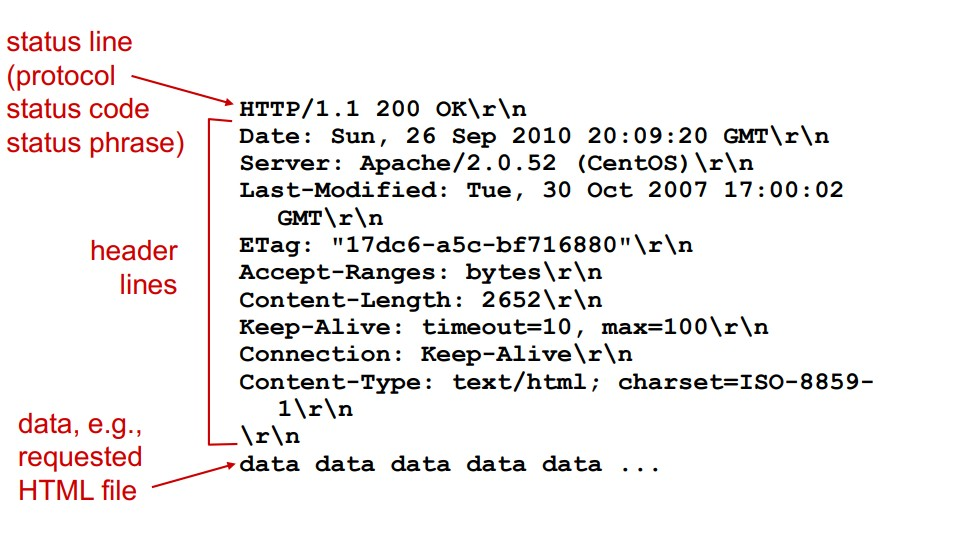
\includegraphics[width=0.5\linewidth]{slide_28.jpg}
    \caption{HTTP response message}
    \label{fig:placeholder}
\end{figure}
Il messaggio di risposta ha una struttura speculare alla richiesta, composta da:

\begin{enumerate}
    \item \textbf{Status Line:} Contiene tre campi:
    \begin{itemize}
        \item La versione del protocollo (es. HTTP/1.1).
        \item Lo \textbf{Status Code} (codice numerico).
        \item La \textbf{Status Phrase} (descrizione testuale, es. "OK").
    \end{itemize}
    
    \item \textbf{Header Lines:} Forniscono metadati sulla risposta (es. \texttt{Date}, \texttt{Server}, \texttt{Content-Length}, \texttt{Content-Type}).
    
    \item \textbf{Entity Body:} Contiene l'oggetto richiesto (es. il codice HTML della pagina, l'immagine, ecc.).
\end{enumerate}

\newpage
\subsubsection{Codici di Stato (Status Codes)}
Il codice di stato appare nella prima linea della risposta per indicare l'esito della richiesta.

\begin{table}[H]
\centering
\begin{tabularx}{\textwidth}{l X}
\toprule
\textbf{Codice} & \textbf{Significato} \\
\midrule
\texttt{200 OK} & La richiesta ha avuto successo e l'oggetto richiesto è incluso nel messaggio. \\
\midrule
\texttt{301 Moved Permanently} & L'oggetto è stato spostato. La nuova posizione è specificata nell'header \texttt{Location}. \\
\midrule
\texttt{400 Bad Request} & Il messaggio di richiesta non è stato compreso dal server (errore generico del client). \\
\midrule
\texttt{404 Not Found} & Il documento richiesto non si trova su questo server. \\
\midrule
\texttt{505 Version Not Supported} & Il server non supporta la versione del protocollo HTTP utilizzata nella richiesta. \\
\bottomrule
\end{tabularx}
\caption{Principali codici di stato HTTP}
\end{table}



\newpage

\subsection*{Gestione dello Stato e Ottimizzazione}

\subsection{Cookies: Mantenere lo Stato in HTTP}
Il protocollo HTTP è nativamente \textbf{stateless} (senza stato): il server non mantiene informazioni sulle richieste passate dello stesso client. Tuttavia, molte applicazioni web (come l'e-commerce) necessitano di identificare gli utenti e mantenere una sessione..

Per risolvere questo problema si utilizzano i \textbf{Cookies}, composti da quattro componenti fondamentali:
\begin{enumerate}
    \item Una riga di header \texttt{Set-cookie:} nel messaggio di \textbf{risposta} HTTP.
    \item Una riga di header \texttt{Cookie:} nel messaggio di \textbf{richiesta} HTTP successivo.
    \item Un file di cookie salvato sull'host dell'utente e gestito dal browser.
    \item Un database di backend sul sito Web per associare l'ID del cookie ai dati dell'utente.
\end{enumerate}

\begin{esempiobox}{Esempio: Accesso a un E-commerce (Amazon)}

\begin{figure}[H]
    \centering
    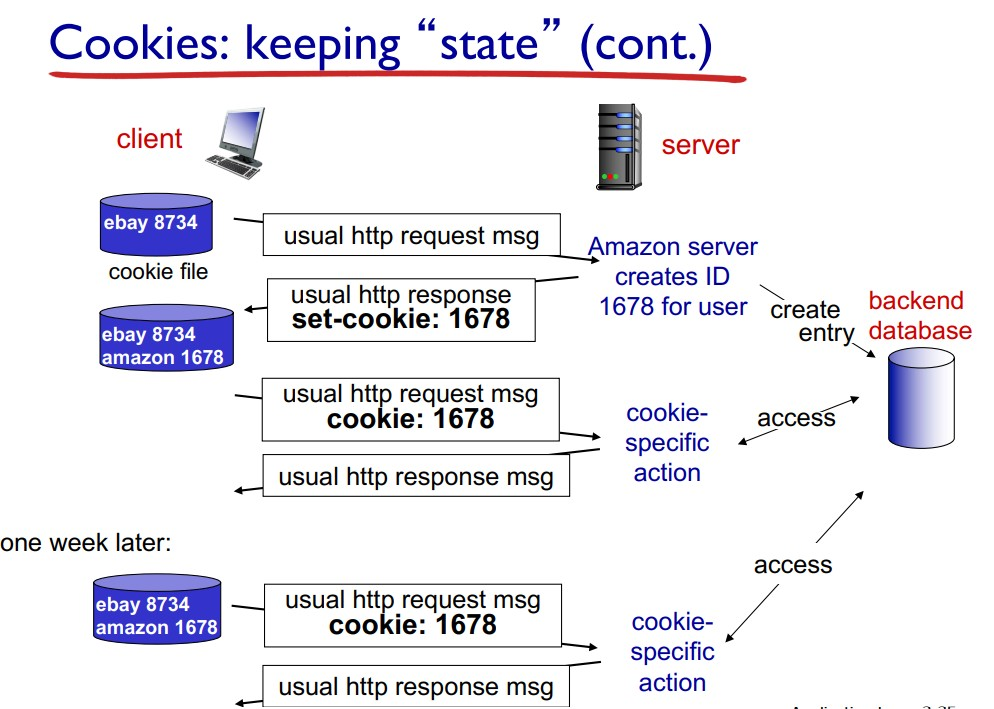
\includegraphics[width=0.5\linewidth]{slide_35.jpg}
    \caption{}
    \label{fig:placeholder}
\end{figure}
    \begin{itemize}
        \item \textbf{Primo Accesso:} Susan visita il sito. Il server crea un ID univoco (es. 1678) e lo memorizza nel database. Risponde con \texttt{Set-cookie: 1678}.
        \item \textbf{Memorizzazione:} Il browser di Susan salva questo ID nel file dei cookie locale.
        \item \textbf{Accessi Successivi:} Quando Susan torna sul sito (anche dopo una settimana), il browser inserisce automaticamente \texttt{Cookie: 1678} nella richiesta.
        \item \textbf{Risultato:} Il server usa l'ID 1678 per recuperare lo stato di Susan dal database (es. il contenuto del carrello o le raccomandazioni).
    \end{itemize}
\end{esempiobox}

\begin{notebox}{Privacy e Cookies}
    I cookie permettono ai siti di imparare molto sulle abitudini degli utenti, sollevando questioni di privacy.
    
    Tuttavia, sono essenziali per funzioni come l'autorizzazione, i carrelli della spesa e le sessioni utente.
\end{notebox}


\newpage
\subsection{Web Caching (Proxy Server) per soddisfare richieste HTTP al posto del server di origine}
Una Web Cache (o Proxy Server) è un'entità di rete che soddisfa le richieste HTTP per conto del server di origine. La cache agisce sia da server (per il client) che da client (per il server di origine).

Il browser invia tutte le richieste HTTP alla cache:
\begin{itemize}
    \item \textbf{Cache Hit:} Se l'oggetto è presente, la cache lo restituisce immediatamente.
    \item \textbf{Cache Miss:} Se l'oggetto non è presente, la cache lo richiede al server di origine e poi lo invia al client, salvandone una copia.
\end{itemize}

\begin{figure} [H]
    \centering
    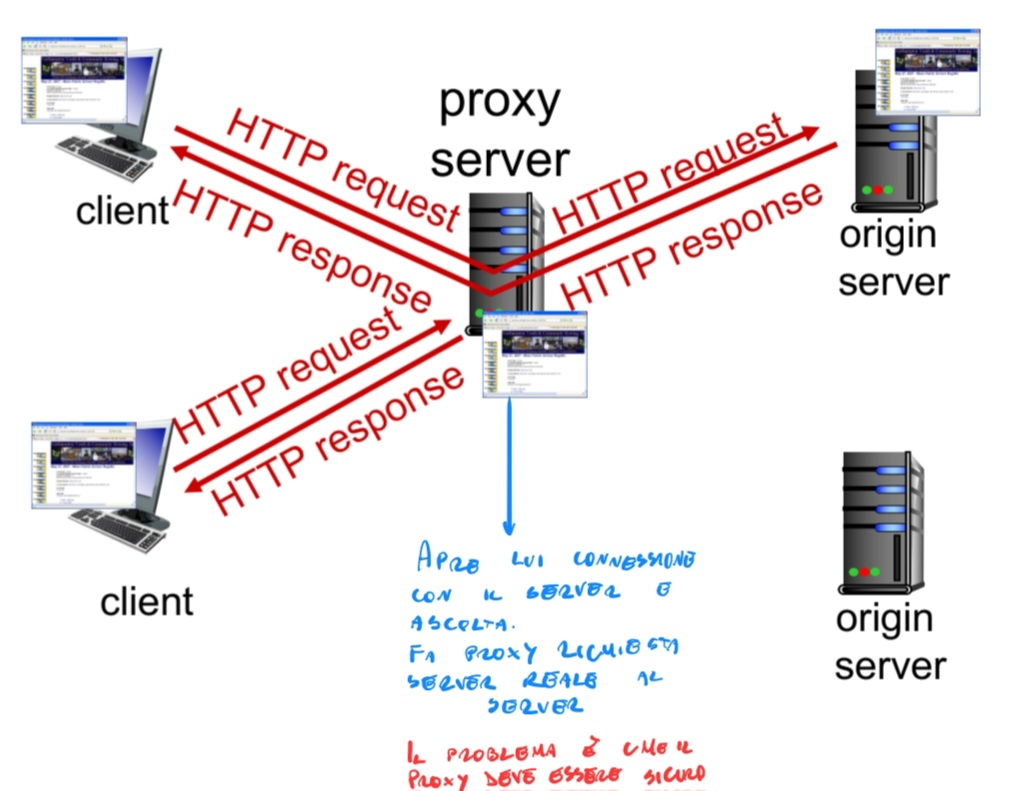
\includegraphics[width=0.5\linewidth]{foto reti di calcolatori/proxy.jpg}
    \label{fig:placeholder}
\end{figure}

\subsubsection{Vantaggi del Caching}
L'utilizzo di cache, spesso installate dagli ISP (Internet Service Provider) o dalle università, offre benefici cruciali:
\begin{itemize}
    \item Riduce i tempi di risposta per il client.
    \item Riduce drasticamente il traffico sul link di accesso istituzionale.
\end{itemize}

\begin{figure}[H]
    \centering
    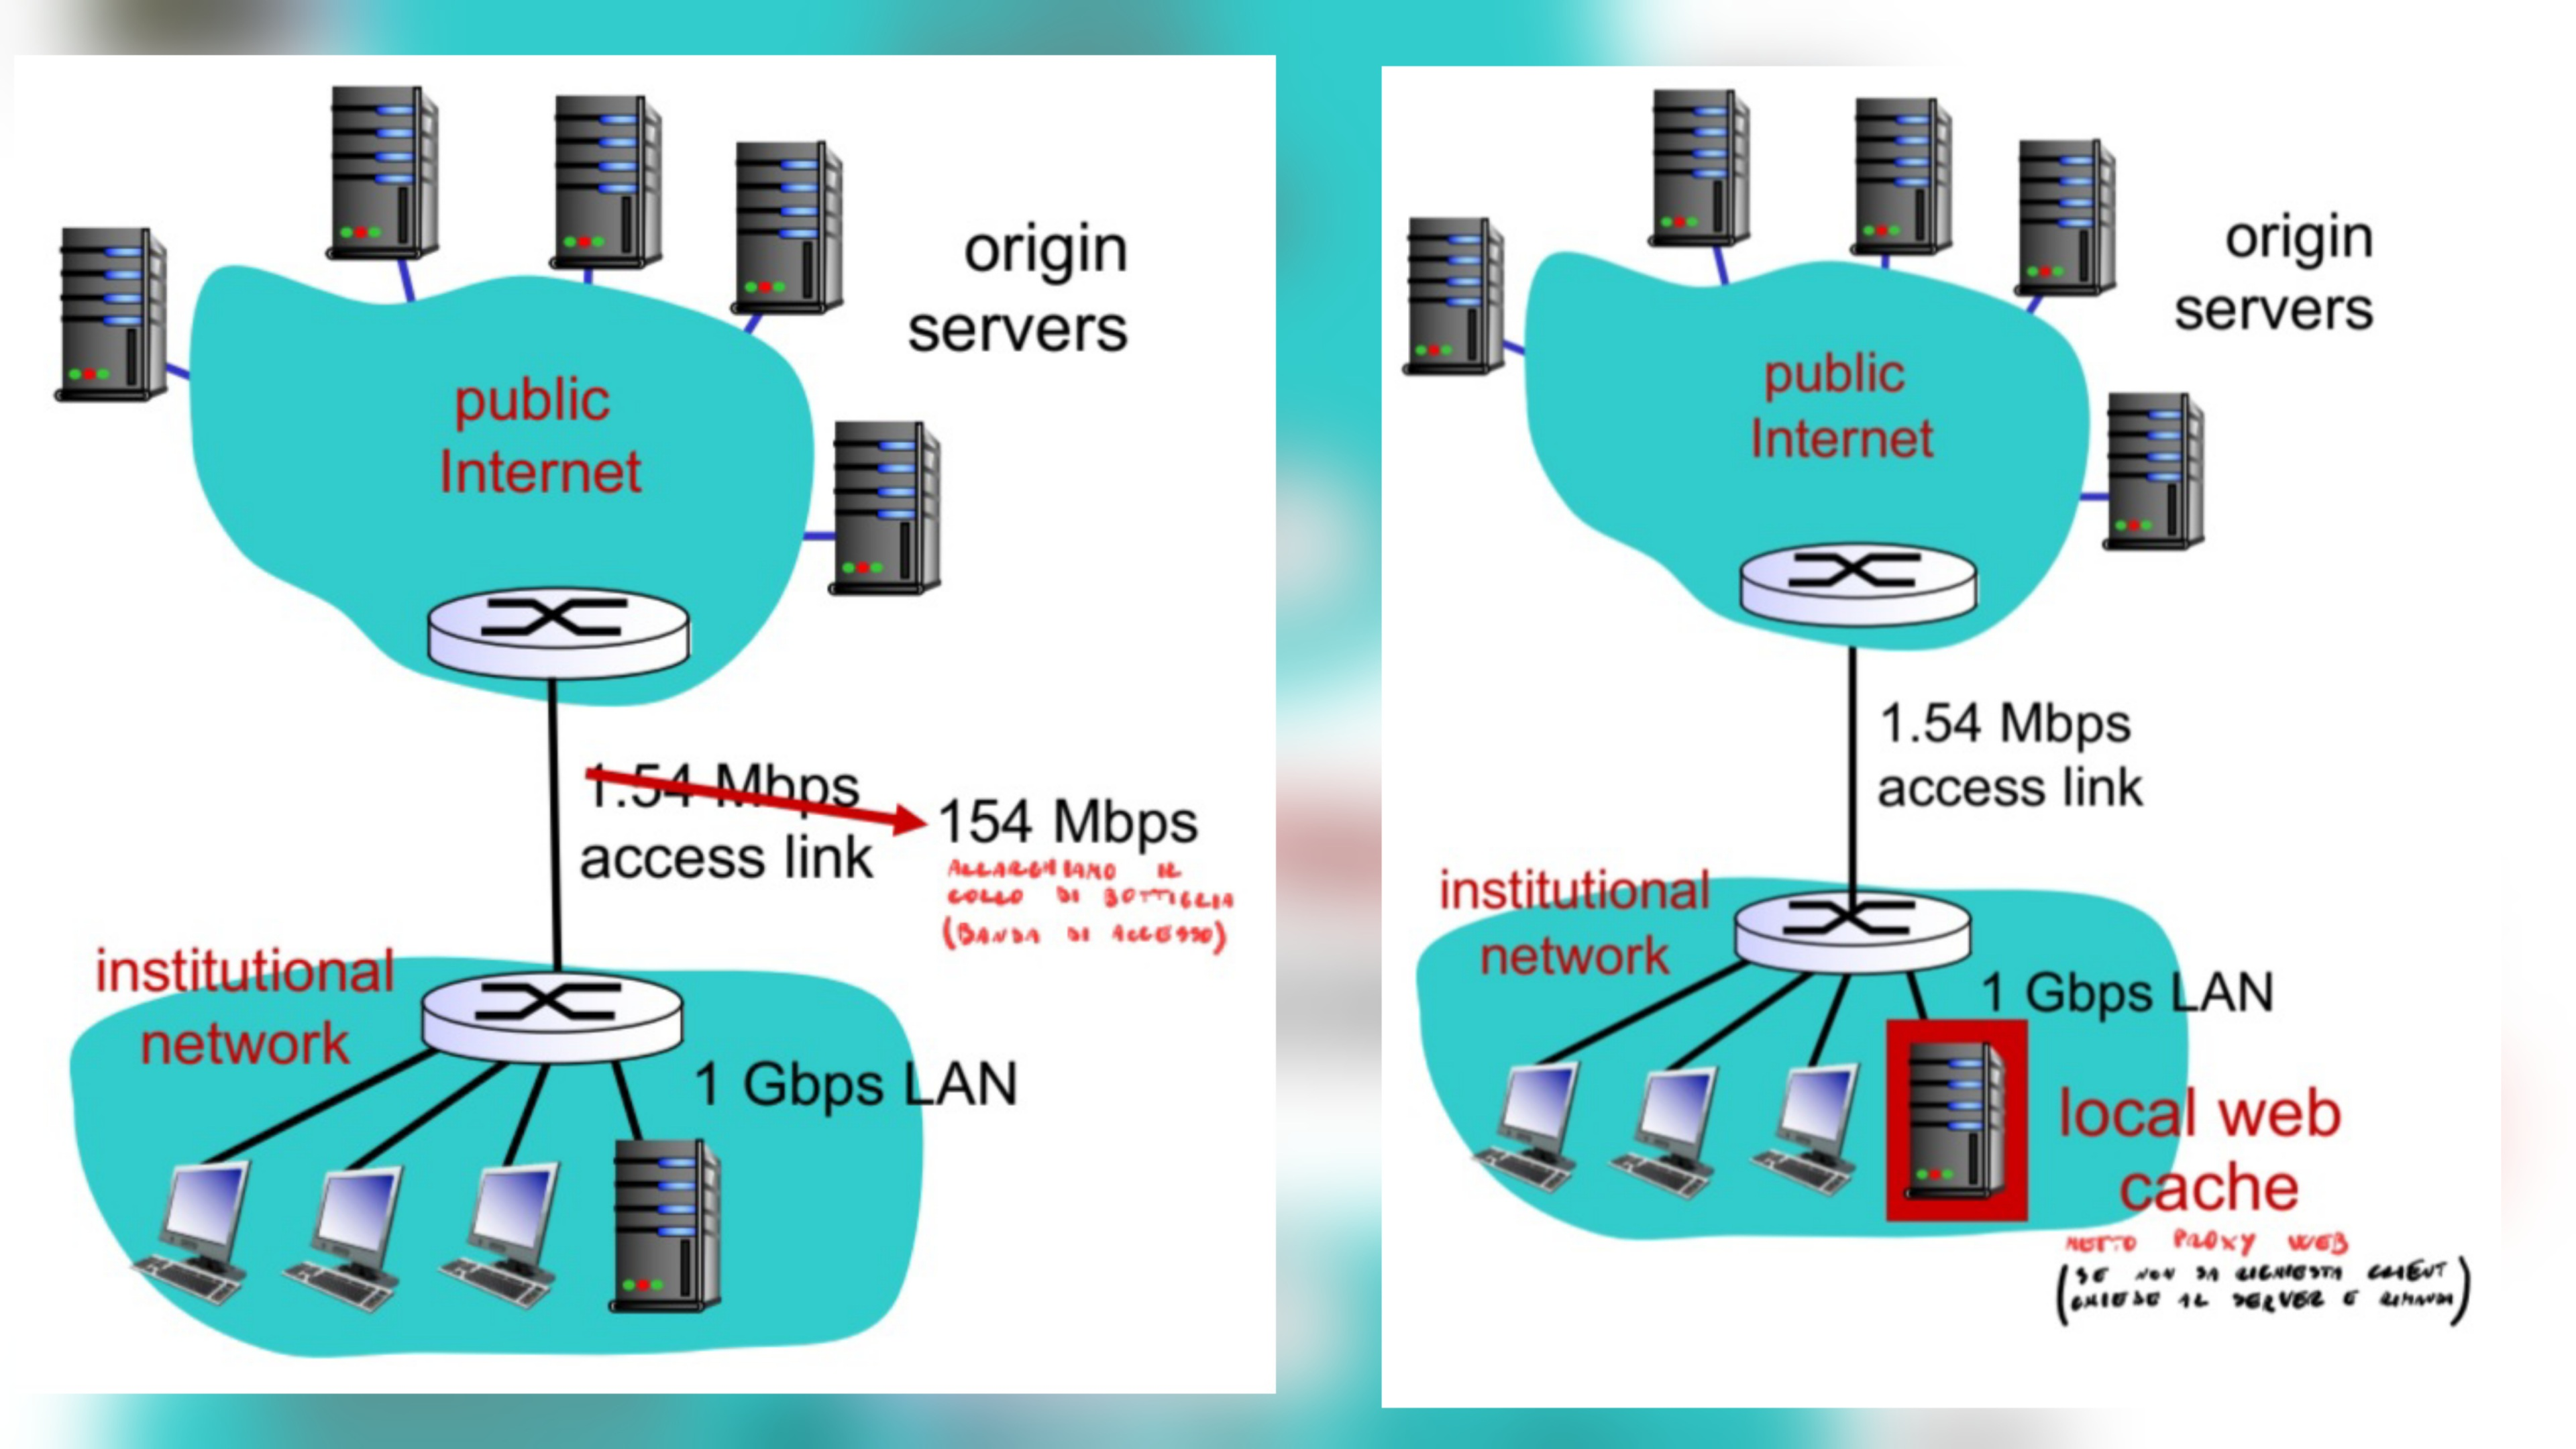
\includegraphics[width=0.7\linewidth]{foto reti di calcolatori/caching.jpg}
    \caption{Confronto tra due soluzioni per risolvere il collo di bottiglia del link di accesso. A sinistra: soluzione costosa che prevede l'aumento della capacità del link fisico (da 1.54 Mbps a 154 Mbps). A destra: soluzione economica che prevede l'installazione di una Web Cache locale (Proxy) per ridurre il traffico sul link esistente.}
    \label{fig:web_caching_solutions}
\end{figure}
\newpage
\begin{esempiobox}{Esempio Quantitativo: Web Caching e Link di Accesso}
    Consideriamo una rete istituzionale con le seguenti caratteristiche:
    
    \textbf{Dati e Assunzioni:}
    \begin{itemize}
        \item \textbf{Dimensione media oggetti:} $100$ Kbit.
        \item \textbf{Tasso medio di richieste:} $15$ richieste/secondo.
        \item \textbf{Ritardo RTT} (Router istituzionale $\to$ Server origine): $2$ secondi.
        \item \textbf{Capacità Link di Accesso:} $1.54$ Mbps.
    \end{itemize}

    \hrulefill

    \paragraph{1. Analisi del Traffico (Senza Cache)}
    Calcoliamo prima quanto traffico genera la rete:
    \[
    \text{Traffico generato} = 15 \text{ rich/sec} \times 100 \text{ kbit/rich} = 1.50 \text{ Mbps}
    \]
    
    Ora calcoliamo l'utilizzo del link di accesso (il "collo di bottiglia"):
    \[
    \text{Utilizzo Link} = \frac{\text{Traffico generato}}{\text{Capacità Link}} = \frac{1.50 \text{ Mbps}}{1.54 \text{ Mbps}} \approx 99\%
    \]
    
    \textbf{Problema:} Con un utilizzo del $99\%$, i ritardi di accodamento (queuing delay) tendono all'infinito. Il tempo totale di risposta per una richiesta sarebbe nell'ordine dei \textbf{minuti}. La navigazione è impossibile.

    \hrulefill
    \paragraph{2. Soluzione "Fatter Access Link"}
    In alternativa all'installazione di una cache, si potrebbe pensare di aumentare drasticamente la capacità del link di accesso.
    
    \textbf{Nuovo Scenario:}
    \begin{itemize}
        \item Traffico medio richiesto: $1.50$ Mbps (invariato).
        \item \textbf{Nuova Capacità Link di Accesso:} Upgrade da $1.54$ Mbps a \textbf{$154$ Mbps} (aumento di fattore 100).
    \end{itemize}


    \paragraph{Analisi delle Prestazioni}
    Con la nuova capacità, ricalcoliamo l'utilizzo del link:
    \[
    \text{Utilizzo Link} = \frac{1.50 \text{ Mbps}}{154 \text{ Mbps}} \approx 0.0099 \approx \mathbf{0.99\%}
    \]
    
    \textbf{Conseguenze sul Ritardo:}
    Poiché l'utilizzo è bassissimo ($< 1\%$), i ritardi di accodamento diventano trascurabili (nell'ordine dei microsecondi).
    \[
    \text{Ritardo Totale} = \text{Ritardo Internet} + \text{Ritardo Accesso} + \text{Ritardo LAN}
    \]
    \[
    \approx 2 \text{ sec} + \text{msecs} + \mu\text{secs} \approx \mathbf{2 \text{ secondi}}
    \]

    \paragraph{Conclusione e Svantaggi}
    Sebbene questa soluzione riduca efficacemente il ritardo a circa 2 secondi (paragonabile alla soluzione con cache), presenta uno svantaggio critico:
    \begin{itemize}
        \item \textbf{Costo Elevato:} Aggiornare un link fisico per moltiplicarne la capacità per 100 comporta costi infrastrutturali e di abbonamento molto alti rispetto all'installazione di una semplice web cache economica.
    \end{itemize}
    

    \hrulefill
    

    \paragraph{3. Soluzione con Web Cache (Proxy)}
    Installiamo una Web Cache locale. Supponiamo che il tasso di successo (\textit{Hit Rate}) sia del \textbf{40\%} ($0.4$).
    Questo significa che:
    \begin{itemize}
        \item Il \textbf{40\%} delle richieste viene soddisfatto immediatamente dalla cache locale (ritardo trascurabile, $\approx 10$ ms).
        \item Il \textbf{60\%} delle richieste deve ancora attraversare il link di accesso per raggiungere i server di origine.
    \end{itemize}

    \textbf{Nuovo carico sul Link di Accesso:}
    \[
    \text{Traffico sul Link} = 0.6 \times 1.50 \text{ Mbps} = 0.90 \text{ Mbps}
    \]

    \textbf{Nuovo Utilizzo del Link:}
    \[
    \text{Utilizzo} = \frac{0.90 \text{ Mbps}}{1.54 \text{ Mbps}} \approx 58\%
    \]
    
    \textbf{Risultato:} Con un utilizzo del $58\%$, il ritardo di accodamento sul link diventa trascurabile (pochi millisecondi). Il ritardo per scaricare dal server di origine rimane quindi dominato dai 2 secondi di RTT Internet (totale $\approx 2.01$ sec).

    \hrulefill

    \paragraph{3. Calcolo del Ritardo Medio Totale}
    Il ritardo medio percepito dall'utente è la media ponderata tra i due casi (Cache Hit e Cache Miss)
    il ritardo Originale indica il ritardo di accesso ad internet, mentre quello di cache il ritardo di comunicazione locale:
    :
    
    \[
    \text{Ritardo Medio} = (\text{Prob. Miss} \times \text{Ritardo Origine}) + (\text{Prob. Hit} \times \text{Ritardo Cache})
    \]
    \[
    \text{Ritardo Medio} = (0.6 \times 2.01 \text{ sec}) + (0.4 \times \approx 0 \text{ sec}) \approx \mathbf{1.2 \text{ secondi}}
    \]

    \textbf{Conclusione:} L'installazione della cache ha ridotto il tempo di risposta da "minuti" a circa 1.2 secondi, senza dover acquistare un costoso link di accesso più veloce (es. upgrade a 154 Mbps).
\end{esempiobox}







\newpage
\subsubsection{Conditional GET ( garantire che gli oggetti nella cache non siano obsoleti )}
Per garantire che gli oggetti nella cache non siano obsoleti (stale), si usa il \textbf{Conditional GET}.
La cache invia una richiesta al server includendo l'header:
\[ \texttt{If-modified-since: <data>} \]
Se l'oggetto non è stato modificato dopo quella data, il server risponde con \textbf{304 Not Modified} e nessun corpo del messaggio (risparmiando banda). Se è cambiato, invia il nuovo oggetto con \textbf{200 OK}.

\begin{figure}[H]
    \centering
    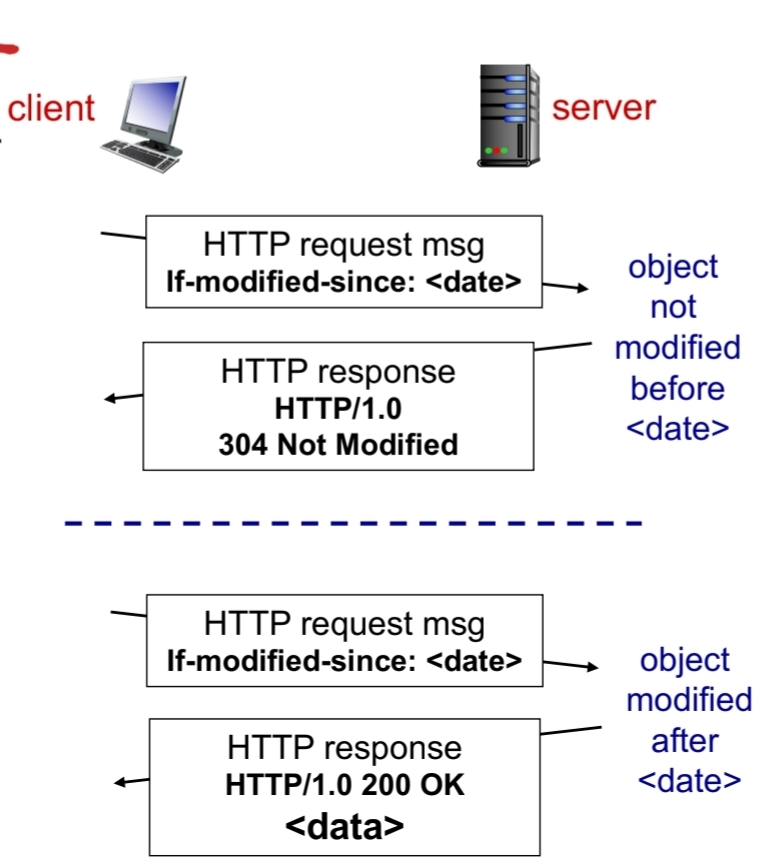
\includegraphics[width=0.5\linewidth]{foto reti di calcolatori/conditional_get.jpg}
    \label{fig:placeholder}
\end{figure}




\newpage
% ===============================================================
\subsection{SMTP, POP3 e IMAP: Posta elettronica}


Il sistema di posta elettronica su Internet si basa su tre componenti principali:
\begin{enumerate}
    \item \textbf{User Agent (UA):} Il software "lettore di posta" (es. Outlook, Thunderbird, Apple Mail) che permette di comporre, leggere e modificare i messaggi.
    \item \textbf{Mail Server:} Il cuore del sistema. Contiene:
    \begin{itemize}
        \item La \textbf{Mailbox}: dove vengono conservati i messaggi in arrivo per l'utente.
        \item La \textbf{Coda dei messaggi}: buffer per i messaggi in uscita che devono essere inviati.
    \end{itemize}
    \item \textbf{SMTP (Simple Mail Transfer Protocol):} Il protocollo utilizzato per scambiare messaggi tra mail server.
\end{enumerate}

\begin{figure}[H]
    \centering
    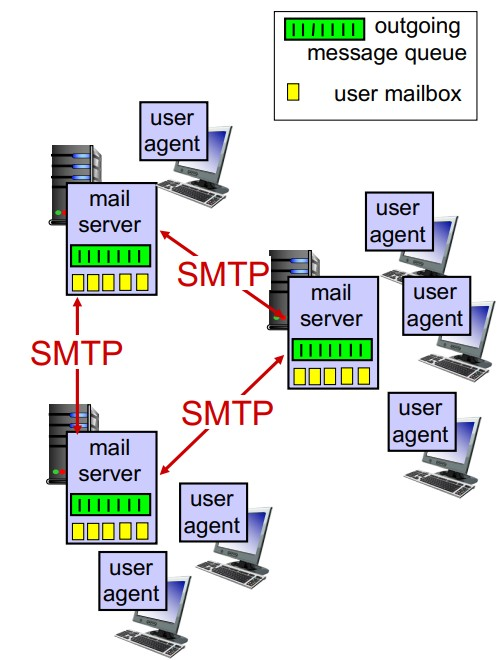
\includegraphics[width=0.4\linewidth]{slide_45.jpg}
    \caption{}
    \label{fig:placeholder}
\end{figure}

\newpage
\subsubsection{SMTP (Simple Mail Transfer Protocol)}
SMTP (RFC 2821) utilizza \textbf{TCP} sulla porta \textbf{25} per trasferire in modo affidabile i messaggi dal client al server. Il trasferimento avviene direttamente dal server del mittente al server del destinatario.

Il protocollo opera in tre fasi distinte:
\begin{enumerate}
    \item \textbf{Handshaking:} Saluto iniziale tra client e server.
    \item \textbf{Trasferimento messaggi:} Scambio effettivo del contenuto.
    \item \textbf{Chiusura (Closure):} Terminazione della connessione.
\end{enumerate}

L'interazione è basata su comandi \textbf{ASCII} (leggibili dall'uomo) e codici di risposta (es. \texttt{220}, \texttt{250 OK}). I messaggi devono essere codificati in ASCII a 7-bit. La fine del messaggio è determinata dalla sequenza \texttt{CRLF.CRLF} (un punto da solo su una riga).

\begin{notebox}{Confronto: HTTP vs SMTP}
    \begin{itemize}
        \item \textbf{HTTP} è un protocollo \textbf{Pull}: il client (browser) tira a sé l'informazione dal server.
        \item \textbf{SMTP} è un protocollo \textbf{Push}: il client (mail server mittente) spinge il messaggio verso il server destinatario.
        \item Entrambi usano comandi ASCII e codici di stato.
        \item SMTP usa connessioni \textbf{persistenti}.
    \end{itemize}
\end{notebox}

\begin{defbox}{Formato del Messaggio}
    Un'email è composta da:
    \begin{itemize}
        \item \textbf{Header:} Linee di intestazione come \texttt{To:}, \texttt{From:}, \texttt{Subject:} (definiti nell'RFC 822). Questi sono diversi dai comandi SMTP (\texttt{MAIL FROM}, \texttt{RCPT TO}).
        \item \textbf{Body:} Il corpo del messaggio (solo caratteri ASCII).
    \end{itemize}
\end{defbox}

\subsubsection{Scenario di Invio: Alice invia a Bob}

\begin{figure}[H]
    \centering
    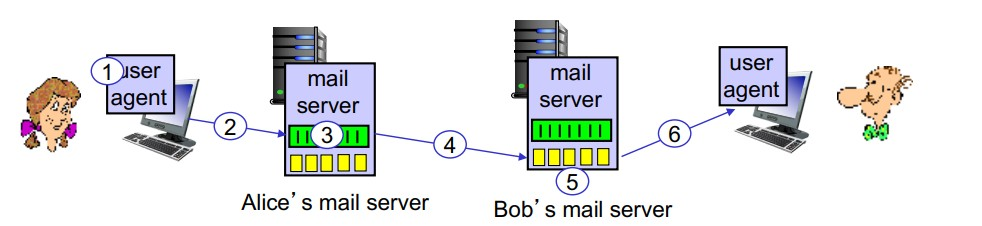
\includegraphics[width=0.7\linewidth]{slide_48.jpg}
    \caption{Caption}
    \label{fig:placeholder}
\end{figure}
\begin{enumerate}
    \item Alice usa il suo UA per comporre il messaggio per \texttt{bob@someschool.edu}.
    \item Lo UA di Alice invia il messaggio al suo mail server (coda).
    \item Il client SMTP (lato server di Alice) apre una connessione TCP con il mail server di Bob.
    \item Il client SMTP invia il messaggio sulla connessione TCP.
    \item Il mail server di Bob mette il messaggio nella mailbox di Bob.
    \item Bob invoca il suo UA per leggere il messaggio.
\end{enumerate}

\newpage
\subsubsection{Protocolli di Accesso alla Posta (Mail Access Protocols)}
Mentre SMTP serve per inviare e trasferire la posta tra server, non è adatto per il recupero da parte dell'utente finale (poiché è un protocollo "push"). Per leggere la posta dal server si usano protocolli di "pull":

\paragraph{1. POP3 (Post Office Protocol - ver 3)}
È un protocollo semplice e \textbf{stateless} (senza stato) tra le sessioni. Funziona in fasi:
\begin{itemize}
    \item \textbf{Autorizzazione:} Il client invia username e password (\texttt{user}, \texttt{pass}).
    \item \textbf{Transazione:} Il client recupera i messaggi.
\end{itemize}

\begin{esempiobox}{Esempio di Sessione POP3}
\textbf{S:} +OK POP3 server ready \\
\textbf{C:} user bob \\
\textbf{S:} +OK \\
\textbf{C:} pass hungry \\
\textbf{S:} +OK user successfully logged on \\
\textbf{C:} list \textit{(elenca i messaggi)} \\
\textbf{S:} 1 498 \textit{(msg 1, dimensione 498 octets)} \\
\textbf{C:} retr 1 \textit{(recupera messaggio 1)} \\
\textbf{C:} dele 1 \textit{(cancella messaggio 1)} \\
\textbf{C:} quit
\end{esempiobox}

POP3 ha due modalità principali:
\begin{itemize}
    \item \textbf{Download and Delete:} Il client scarica e cancella dal server. L'utente non può rileggere la mail da un altro dispositivo.
    \item \textbf{Download and Keep:} Il client scarica ma lascia una copia sul server.
\end{itemize}

\vspace{1cm}
\paragraph{2. IMAP (Internet Mail Access Protocol)}
Più complesso di POP3. Mantiene tutti i messaggi sul server, permettendo all'utente di organizzarli in cartelle.
\begin{itemize}
    \item Mantiene lo \textbf{stato} dell'utente tra le sessioni (es. nomi delle cartelle, quali messaggi sono stati letti).
    \item Permette di spostare messaggi da una cartella all'altra.
\end{itemize}

\vspace{1cm}
\paragraph{3. HTTP (Webmail)}
Gmail, Outlook.com, ecc. usano HTTP per permettere all'utente di accedere alla mailbox tramite browser.
% ===============================================================

\newpage
\subsection{DHCP: Dynamic Host Configuration Protocol}
\label{sec:DHCP}


\begin{defbox}{DHCP -- Dynamic Host Configuration Protocol}
\textbf{DHCP} permette a un host di ottenere \textbf{dinamicamente} il
proprio indirizzo IP (e altre configurazioni di rete) da un server quando
si connette alla rete. È un protocollo \textit{plug-and-play}.
\end{defbox}
Il protocollo DHCP consente di assegnare automaticamente:
\begin{itemize}
    \item indirizzo IP,
    \item gateway,
    \item subnet mask,
    \item DNS server,
    \item altri parametri di rete.
\end{itemize}

\begin{notebox}{Perché è necessario}
Senza DHCP la configurazione di rete andrebbe eseguita manualmente,
rischiando errori e conflitti di indirizzi.
\end{notebox}

\newpage
% ===============================================================
\subsection{Architetture dei Servizi: Client/Server e Peer to Peer}

Le applicazioni e i servizi su Internet non sono tutti uguali: il modo in cui gli host interagiscono tra loro definisce l'\textbf{architettura logica} dell'applicazione. Esistono due paradigmi fondamentali: l'architettura \textbf{Client/Server} e l'architettura \textbf{Peer to Peer (P2P)}.

% Disegno TIKZ per rappresentare le due architetture
\begin{figure}[H]
    \centering
    \begin{tikzpicture}[scale=0.8, transform shape]
        % --- CLIENT SERVER ---
        \node (server) at (0,0) [circle, draw=blue, fill=blue!10, thick, minimum size=1.2cm] {\textbf{S}};
        \node (c1) at (-2,1) [circle, draw=black, fill=white, minimum size=0.8cm] {C};
        \node (c2) at (-2,-1) [circle, draw=black, fill=white, minimum size=0.8cm] {C};
        \node (c3) at (2,1) [circle, draw=black, fill=white, minimum size=0.8cm] {C};
        \node (c4) at (2,-1) [circle, draw=black, fill=white, minimum size=0.8cm] {C};
        
        \draw[<->, thick] (server) -- (c1);
        \draw[<->, thick] (server) -- (c2);
        \draw[<->, thick] (server) -- (c3);
        \draw[<->, thick] (server) -- (c4);
        
        \node at (0, -2.5) {\textbf{Architettura Client/Server}};
        
        % --- P2P ---
        \begin{scope}[xshift=8cm]
            \node (p1) at (0,1.5) [circle, draw=orange, fill=orange!10, thick, minimum size=0.8cm] {};
            \node (p2) at (-1.5,0.5) [circle, draw=orange, fill=orange!10, thick, minimum size=0.8cm] {};
            \node (p3) at (-1,-1.2) [circle, draw=orange, fill=orange!10, thick, minimum size=0.8cm] {};
            \node (p4) at (1,-1.2) [circle, draw=orange, fill=orange!10, thick, minimum size=0.8cm] {};
            \node (p5) at (1.5,0.5) [circle, draw=orange, fill=orange!10, thick, minimum size=0.8cm] {};
            
            \draw[<->] (p1) -- (p2);
            \draw[<->] (p1) -- (p5);
            \draw[<->] (p2) -- (p3);
            \draw[<->] (p3) -- (p4);
            \draw[<->] (p4) -- (p5);
            \draw[<->] (p2) -- (p4); % connessione interna
            \draw[<->] (p2) -- (p5); % connessione interna
            
            \node at (0, -2.5) {\textbf{Architettura Peer to Peer}};
        \end{scope}
    \end{tikzpicture}
    \caption{Confronto visuale: nel modello C/S il server è il centro delle comunicazioni; nel P2P ogni nodo comunica direttamente con gli altri.}
\end{figure}

% ------------------------------------------------

\subsubsection{Architettura Client/Server}

È il modello tradizionale e più diffuso su Internet. Prevede una netta distinzione di ruoli tra gli host che partecipano alla comunicazione.

\begin{defbox}{Ruoli nel Client/Server}
\begin{itemize}
    \item \textbf{Client:} Host che avviano la comunicazione spedendo richieste di servizio. Attendono una risposta.

     può essere connesso in modo intermittente e avere indirizzo IP dinamico. I client non comunicano direttamente tra loro.
    \item \textbf{Server:} Host sempre attivi (spesso con indirizzo IP fisso) su cui sono in esecuzione i servizi. Attendono passivamente le richieste e le soddisfano.

    Spesso risiede in data center per garantire scalabilità.
\end{itemize}
\end{defbox}

In questo modello, il Server è l'unico destinatario possibile per le richieste dei client. I client non comunicano direttamente tra loro.

\begin{esempiobox}{Esempi di Client/Server}
\begin{itemize}
    \item \textbf{World Wide Web (HTTP):} Il browser (client) chiede una pagina al Web Server.
    \item \textbf{Email:} Il client di posta invia mail al server SMTP o scarica dal server POP3/IMAP.
    \item \textbf{DNS:} L'host chiede la risoluzione di un nome al server DNS.
\end{itemize}
\end{esempiobox}

\newpage
% -----------
\subsubsection{Architettura Peer to Peer (P2P)}

Nell'architettura P2P non esiste una distinzione fissa tra chi chiede e chi fornisce il servizio. Questa architettura è altamente scalabile ma più complessa da gestire.

\begin{defbox}{Caratteristiche P2P}
Tutti gli host sono considerati ``pari'' (\textit{peers}).
\begin{itemize}
    \item Ogni host è \textbf{contemporaneamente sia Client che Server}.
    \item Agisce da \textbf{Server} quando fornisce risorse o risposte ad altri peer.
    \item Agisce da \textbf{Client} quando invia richieste ad altri host (per sé o per conto terzi).
\end{itemize}

Questo comporta che:

\begin{itemize}
    \item Nessun server sempre attivo.
    \item Sistemi finali arbitrari comunicano direttamente tra loro.
    \item \textbf{Auto-scalabilità:} I nuovi peer portano nuova capacità di servizio oltre a nuove richieste.
    \item Gestione complessa a causa della connettività intermittente e del cambio di indirizzi IP.
\end{itemize}
\end{defbox}

Nel P2P puro, non esiste un server centrale: la rete è formata dalle connessioni dirette tra gli utenti finali.

\textbf{Esempi:} Distribuzione file (BitTorrent), Streaming (Kankan), VoIP (Skype).

\newpage
\subsection*{Esempio distribuzione di un file C/S  vs  P2P}

\begin{figure}[H]
    \centering
    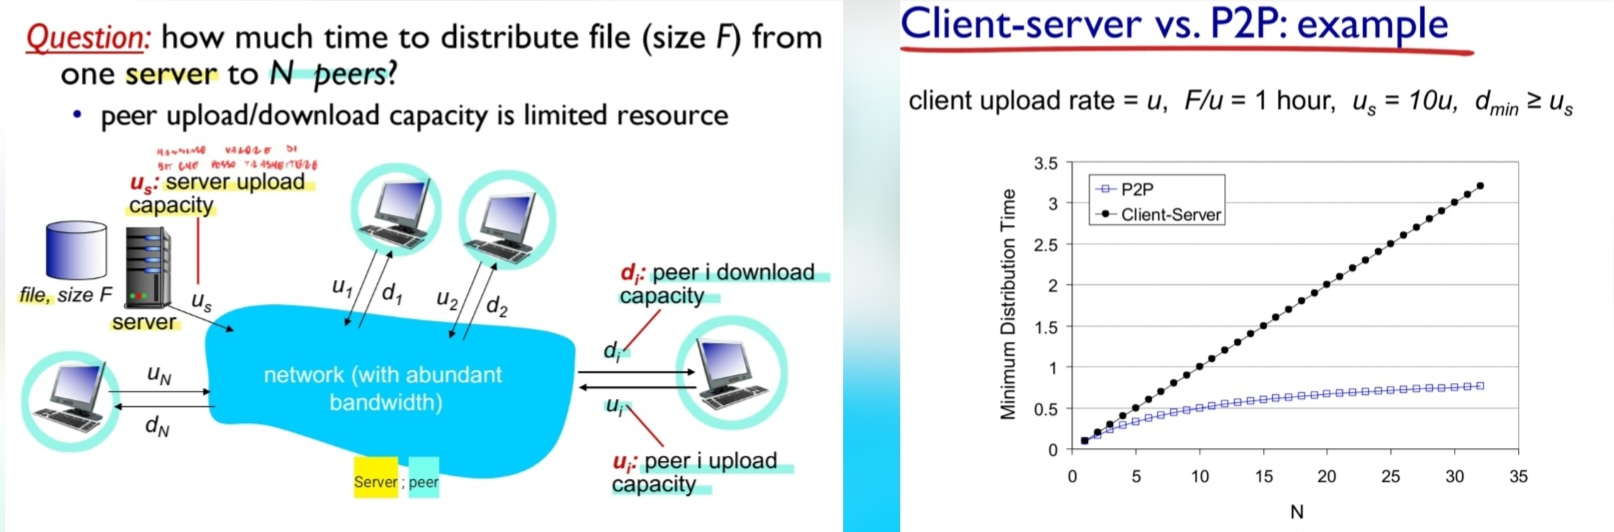
\includegraphics[width=1\linewidth]{foto reti di calcolatori/P2P.jpg}
    \label{fig:placeholder}
\end{figure}

\begin{esempiobox}{Analisi dei Tempi di Distribuzione}

Il problema fondamentale analizzato è: \textit{Quanto tempo occorre per distribuire un file di dimensione $F$ da un server a $N$ peers?}.

\subsection*{Definizione delle Variabili}
\begin{itemize}
    \item $u_s$: Capacità di upload del server.
    \item $u_i$: Capacità di upload del peer $i$.
    \item $d_i$: Capacità di download del peer $i$.
    \item $d_{min}$: La minima capacità di download tra i client.
    \item $F$: Dimensione del file.
    \item $N$: Numero di peer.
\end{itemize}

\subsection*{Modello Client-Server}
In questo modello, il server deve inviare sequenzialmente $N$ copie del file.
\begin{itemize}
    \item \textbf{Server}: Tempo per inviare $N$ copie: $NF / u_s$.
    \item \textbf{Client}: Tempo per un client per scaricare il file: $F / d_{min}$.
\end{itemize}

Il tempo di distribuzione minimo $D_{c-s}$ è dato dal massimo tra il collo di bottiglia del server(ovvero quanto è lento il server a fare upload) e quello del client più lento a scaricare:

\begin{equation}
D_{c-s} \ge \max \left\{ \frac{NF}{u_s}, \frac{F}{d_{min}} \right\}
\end{equation}

\textbf{Conclusione:} Il tempo aumenta \textbf{linearmente} con $N$ (numero di peer). Se $N$ raddoppia, il tempo raddoppia.

\newpage
\subsection*{Modello P2P}
In questo modello, ogni peer contribuisce alla ridistribuzione caricando parti del file ad altri peer (servizio cooperativo).
\begin{itemize}
    \item Il server deve inviare almeno una copia: $F / u_s$.
    \item Il client deve scaricare una copia: $F / d_{min}$.
    \item La capacità totale di upload del sistema è la somma di quella del server e di tutti i peer: $u_{total} = u_s + \sum_{i=1}^{N} u_i$.
\end{itemize}

Il tempo di distribuzione minimo $D_{P2P}$ è:

\begin{equation}
D_{P2P} \ge \max \left\{ \frac{F}{u_s}, \frac{F}{d_{min}}, \frac{NF}{u_s + \sum_{i=1}^{N} u_i} \right\}
\end{equation}

\textbf{Conclusione:} All'aumentare di $N$, anche il denominatore (capacità totale) aumenta. Poiché ogni peer porta capacità di servizio, il tempo di distribuzione rimane pressoché \textbf{costante} indipendentemente dal numero di utenti (scalabilità perfetta).

\end{esempiobox}



\newpage
% ------------------------------------------------
% SEZIONE BITTORRENT (Case Study)
% ------------------------------------------------
\subsection*{Implementazione Reale: Il protocollo BitTorrent}

L'analisi matematica precedente dimostra la superiorità del P2P nella distribuzione di grandi file. L'esempio più celebre di questa applicazione è \textbf{BitTorrent}.

\begin{esempiobox}{Case Study: BitTorrent}

BitTorrent è un protocollo per la distribuzione di file P2P che gestisce la complessità della rete attraverso meccanismi specifici.

\subsection*{Componenti e Funzionamento}
\begin{itemize}
    \item \textbf{Chunks:} Il file originale non viene scambiato intero, ma diviso in pezzi (chunks) di dimensione fissa (tipicamente \textbf{256 Kb}).
    \item \textbf{Tracker:} Un server infrastrutturale che tiene traccia dei peer che partecipano al torrent. Quando un nuovo peer (es. Alice) si unisce, contatta il tracker per ottenere una lista di IP di altri peer con cui scambiare dati.
    \item \textbf{Torrent:} L'insieme dei peer che stanno scambiando i chunk di uno specifico file.
    \item \textbf{Churn:} La rete è dinamica. I peer entrano ed escono continuamente. Una volta che un peer ha scaricato l'intero file, può decidere di disconnettersi (\textit{egoista}) o rimanere nel torrent per inviare chunk ad altri (\textit{altruista} o \textit{seeder}).
\end{itemize}

\subsection*{Strategie di Scambio (Intelligence)}
Il protocollo deve decidere \textit{quali} pezzi richiedere e a \textit{chi} inviarli.

\subsubsection*{1. Richiesta: Rarest First (Prima i più rari)}
A un dato istante, peer diversi possiedono sottoinsiemi diversi di chunk.
\begin{itemize}
    \item \textbf{Problema:} Evitare che i chunk rari vadano persi se i pochi peer che li hanno si disconnettono.
    \item \textbf{Soluzione:} Alice chiede periodicamente ai vicini quali chunk hanno. Richiede per primi i chunk che sono posseduti dal minor numero di vicini. Questo ridistribuisce rapidamente le copie rare, livellando la disponibilità.
\end{itemize}

\subsubsection*{2. Invio: Tit-for-Tat (Occhio per occhio)}
Questa strategia serve a incentivare la cooperazione ed evitare il \textit{free-riding} (scaricare senza contribuire).
\begin{itemize}
    \item Alice invia dati (upload) solo a un sottoinsieme di peer (tipicamente i \textbf{top 4}) che le stanno inviando dati alla velocità maggiore.
    \item Gli altri peer vengono \textbf{strozzati} (\textit{choked}): non ricevono dati da Alice.
    \item La classifica dei "top 4" viene ricalcolata ogni 10 secondi.
\end{itemize}

\subsubsection*{3. Scoperta: Optimistic Unchoking}
C'è il rischio di rimanere bloccati con partner lenti.
\begin{itemize}
    \item \textbf{Meccanismo:} Ogni \textbf{30 secondi}, Alice seleziona casualmente un peer "strozzato" e inizia a inviargli dati (\textit{optimistically unchoke}).
    \item \textbf{Scopo:} Verificare se questo nuovo partner ha una velocità di upload migliore rispetto ai 4 attuali. Se sì, entrerà nella top 4 al prossimo giro di \textit{Tit-for-Tat}.
\end{itemize}

\end{esempiobox}

% ------------------------------------------------
% CONCLUSIONE DI CONFRONTO
% ------------------------------------------------
\vspace{1cm}

\subsection*{Sintesi Finale: Client/Server vs Peer to Peer}

Possiamo riassumere le differenze strutturali e prestazionali dei due paradigmi nella seguente tabella di confronto:

\begin{table}[H]
    \centering
    \renewcommand{\arraystretch}{1.5} % Aumenta lo spazio tra le righe
    \begin{tabular}{|p{0.25\linewidth}|p{0.35\linewidth}|p{0.35\linewidth}|}
        \hline
        \textbf{Caratteristica} & \textbf{Client / Server} & \textbf{Peer to Peer (P2P)} \\
        \hline
        \textbf{Ruoli} & Ben distinti e asimmetrici. Il client richiede, il server fornisce. & Simmetrici. Ogni nodo è sia client che server . \\
        \hline
        \textbf{Scalabilità} & \textbf{Limitata.} Le prestazioni degradano all'aumentare dei client (collo di bottiglia sul server). & \textbf{Elevata.} Ogni nuovo nodo porta nuova capacità di calcolo e banda (auto-scalabilità). \\
        \hline
        \textbf{Gestione} & Centralizzata e semplificata (basta gestire il server). & Decentralizzata e complessa (richiede protocolli sofisticati di gestione distribuita). \\
        \hline
        \textbf{Affidabilità} & \textit{Single Point of Failure}: se il server cade, il servizio si ferma. & Robusta: se un peer cade, gli altri continuano a funzionare. \\
        \hline
        \textbf{Indirizzamento} & Il server necessita di IP statico/fisso. & I peer possono avere IP dinamici e connettività intermittente. \\
        \hline
    \end{tabular}
    \caption{Confronto riassuntivo tra le architetture di rete.}
    \label{tab:confronto_cs_p2p}
\end{table}

In conclusione, l'architettura \textbf{Client/Server} è ideale per servizi che richiedono controllo centralizzato, sicurezza e dati aggiornati in tempo reale (es. Web, Banking). L'architettura \textbf{P2P} è superiore per la distribuzione massiva di dati e risorse dove la scalabilità è il requisito primario (es. File Sharing, Blockchain, VoIP).

\newpage
% ------------------------------------------------
\subsubsection{Architetture Ibride}

Esistono servizi che tentano di combinare i vantaggi di entrambi i paradigmi (l'affidabilità del Client/Server e la scalabilità del P2P).

In un \textbf{servizio ibrido}, si attua un disaccoppiamento tra le informazioni di controllo e il contenuto vero e proprio:

\begin{itemize}
    \item \textbf{Piano di Controllo (Centralizzato):} Esistono dei \textbf{Server centralizzati} che gestiscono funzioni critiche ma "leggere" come:
    \begin{itemize}
        \item Autenticazione degli utenti (Login).
        \item Mantenimento dell'indice delle risorse (chi possiede cosa).
        \item Ricerca dei contenuti.
    \end{itemize}
    \item \textbf{Piano dei Dati (Distribuito):} Il trasferimento effettivo dei file (pesanti) o lo streaming audio/video avviene in modalità \textbf{P2P} (direttamente tra gli utenti), senza passare per il server centrale.
\end{itemize}

\begin{notebox}[Caso storico: Napster]
\textbf{Napster} (1999) fu il primo famoso esempio di architettura ibrida per il file-sharing musicale.

\textbf{Funzionamento:}
\begin{enumerate}
    \item \textbf{Login:} Quando un utente (Alice) avviava il software, si connetteva al server centrale e inviava la lista dei suoi file MP3.
    \item \textbf{Indicizzazione:} Il server centrale aggiornava il database globale: \textit{"Alice (IP X) ha la canzone Y"}.
    \item \textbf{Ricerca:} Bob chiedeva al server: \textit{"Chi ha la canzone Y?"}. Il server rispondeva: \textit{"Ce l'ha Alice all'indirizzo IP X"}.
    \item \textbf{Scambio (P2P):} Bob si connetteva direttamente ad Alice per scaricare il file. Il file MP3 non passava mai dal server.
\end{enumerate}

\textbf{Punto Debole:} Il server centrale rappresentava un \textit{Single Point of Failure}. Quando il server fu chiuso per vie legali, la rete smise di funzionare perché i peer non riuscivano più a trovarsi, nonostante avessero ancora i file.
\end{notebox}

\paragraph{Vantaggi e Svantaggi:}
\begin{itemize}
    \item \textbf{Pro:} La ricerca è veloce ed efficiente (grazie al server centrale) e il trasferimento non intasa il server (grazie al P2P).
    \item \textbf{Contro:} Se il server di indicizzazione cade o viene spento, la rete diventa inutilizzabile (problema che non esiste nel P2P puro come BitTorrent).
\end{itemize}








%=========================================0
% ------------------------------------------------
% SEZIONE VIDEO STREAMING E CDN
% ------------------------------------------------
\newpage
\subsection{Applicazioni Multimediali: Video Streaming e CDN}

Il traffico video rappresenta oggi la maggior parte del consumo di banda su Internet (es. Netflix e YouTube). La sfida principale non è solo trasmettere dati, ma farlo in modo scalabile verso milioni di utenti con connessioni eterogenee.

% Disegno TIKZ per rappresentare il concetto di CDN
\begin{figure}[H]
    \centering
    \begin{tikzpicture}[scale=0.8, transform shape]
        % --- SENZA CDN ---
        \node (origin) at (0,2) [rectangle, draw=red, fill=red!10, thick, minimum size=1cm] {\textbf{Server Unico}};
        \node (net) at (0,0) [cloud, draw=gray, aspect=2, minimum width=3cm] {Internet};
        \node (user1) at (-2,-2) [circle, draw=black, fill=white] {U};
        \node (user2) at (2,-2) [circle, draw=black, fill=white] {U};
        
        \draw[->, thick, red, dashed] (origin) -- (net);
        \draw[->, thick, red, dashed] (net) -- (user1);
        \draw[->, thick, red, dashed] (net) -- (user2);
        
        \node at (0, -3) {\textbf{Approccio Centralizzato (Collo di bottiglia)}};
        
        % --- CON CDN ---
        \begin{scope}[xshift=8cm]
            \node (origin2) at (0,2) [rectangle, draw=blue, fill=blue!10, thick, minimum size=1cm] {\textbf{Origin}};
            \node (cdn1) at (-2,0) [rectangle, draw=green!60!black, fill=green!10, thick] {CDN Node};
            \node (cdn2) at (2,0) [rectangle, draw=green!60!black, fill=green!10, thick] {CDN Node};
            
            \node (u1) at (-2,-2) [circle, draw=black, fill=white] {U};
            \node (u2) at (2,-2) [circle, draw=black, fill=white] {U};
            
            \draw[->, thick, blue] (origin2) -- (cdn1); % Copia
            \draw[->, thick, blue] (origin2) -- (cdn2); % Copia
            \draw[->, thick, green!60!black] (cdn1) -- (u1); % Streaming locale
            \draw[->, thick, green!60!black] (cdn2) -- (u2); % Streaming locale
            
            \node at (0, -3) {\textbf{Architettura CDN (Distribuita)}};
        \end{scope}
    \end{tikzpicture}
    \caption{Confronto: il server unico soffre di congestione e distanza; la CDN porta il contenuto vicino all'utente.}
\end{figure}

% ------------------------------------------------
\subsubsection{La Codifica e lo Streaming DASH (Dynamic, Adaptive Streaming over HTTP)}

Un video è definito come una sequenza di immagini digitali (array di pixel) visualizzate a un tasso costante (es. 24 immagini al secondo). Poiché ogni pixel è rappresentato da bit, la quantità di dati grezzi è enorme. Per ridurre i bit necessari alla trasmissione, la codifica sfrutta la \textbf{ridondanza} presente nelle immagini.

\begin{defbox}{Compressione Video: Tipi di Codifica}
Per comprimere il video, si agisce su due livelli di ridondanza:

\begin{itemize}
    \item \textbf{Ridondanza Spaziale (all'interno dell'immagine):} Sfrutta la ripetizione di valori nello stesso frame.
    \begin{itemize}
        \item \textit{Esempio:} Invece di inviare $N$ valori identici per un colore (es. tutti viola), si inviano solo due valori: il valore del colore (viola) e il numero di ripetizioni ($N$).
    \end{itemize}
    
    \item \textbf{Ridondanza Temporale (tra immagini successive):} Sfrutta il fatto che frame consecutivi sono spesso simili.
    \begin{itemize}
        \item \textit{Esempio:} Invece di inviare l'intero frame $i+1$, si inviano solo le differenze (i delta) rispetto al frame precedente $i$.
    \end{itemize}
\end{itemize}

Il flusso di bit risultante (encoding rate) può essere gestito in due modi:
\begin{itemize}
    \item \textbf{CBR (Constant Bit Rate):} Il tasso di codifica è fisso (es. MPEG 1 per CD-ROM a 1.5 Mbps).
    \item \textbf{VBR (Variable Bit Rate):} Il tasso cambia dinamicamente in base alla complessità spaziale e temporale della scena (es. MPEG 4 per Internet, spesso < 1 Mbps).
\end{itemize}
\end{defbox}

La tecnica dominante oggi per lo streaming è il \textbf{DASH} (Dynamic, Adaptive Streaming over HTTP).

\begin{defbox}{Funzionamento DASH}
Invece di scaricare un file intero, il flusso è adattivo e l'\textbf{intelligenza} è spostata interamente sul client.

\begin{itemize}
    \item \textbf{Lato Server:}
    \begin{itemize}
        \item Divide il file video in multipli segmenti (\textit{chunks}).
        \item Ogni chunk è memorizzato e codificato a \textbf{differenti tassi} (bitrate differenti).
        \item Fornisce un \textbf{manifest file} che contiene gli URL per i diversi chunks.
    \end{itemize}

    \item \textbf{Lato Client ("Intelligence"):}
    Il client misura periodicamente la banda disponibile e decide dinamicamente chunk per chunk:
    \begin{enumerate}
        \item \textbf{Quando} richiederlo: per gestire il buffer evitando che si svuoti (interruzione video) o vada in overflow.
        \item \textbf{Cosa} richiedere: sceglie il massimo tasso di codifica sostenibile in quel momento (alta qualità se c'è banda, bassa se la rete è congestionata).
        \item \textbf{Dove} richiederlo: può scegliere un server URL specifico che sia fisicamente più "vicino" o che abbia maggiore disponibilità di banda.
    \end{enumerate}
\end{itemize}

\textbf{Vantaggio pratico:} Questa architettura garantisce la continuità del servizio tra dispositivi diversi. Ad esempio, è possibile iniziare uno streaming sulla TV (connessa al Wi-Fi) e continuarlo fluidamente sullo smartphone (passando al 4G) uscendo di casa: il nuovo client riprenderà semplicemente a chiedere i chunk successivi adattandosi alla nuova capacità di rete.
\end{defbox}

\vspace{1cm}
\subsubsection{Content Distribution Networks (CDN)}

Come fa un servizio come YouTube a servire un miliardo di utenti contemporaneamente? Un singolo mega-server non è scalabile (singolo punto di guasto, congestione, lentezza per utenti lontani).

La soluzione è la \textbf{CDN}: una rete di server geograficamente distribuiti che memorizzano copie dei contenuti.

\begin{defbox}{Strategie di Posizionamento CDN}
Esistono due filosofie principali per posizionare i server:
\begin{itemize}
    \item \textbf{Enter Deep (es. Akamai):} Posizionare migliaia di piccoli cluster di server \textit{dentro} le reti di accesso degli ISP residenziali. 
    \textit{Pro:} Vicinanza estrema all'utente. \textit{Contro:} Gestione complessa.
    \item \textbf{Bring Home (es. Limelight):} Creare pochi cluster molto grandi (decine) posizionati nei punti nevralgici di interscambio (POP), vicino alle reti di accesso ma non dentro.
    
    \textit{Pro:} Manutenzione più semplice. \textit{Contro:} Leggermente più distanti dall'utente finale.
\end{itemize}
\end{defbox}

\newpage
\subsubsection{La Logica della Distribuzione Geografica}


\begin{figure}[H]
    \centering
    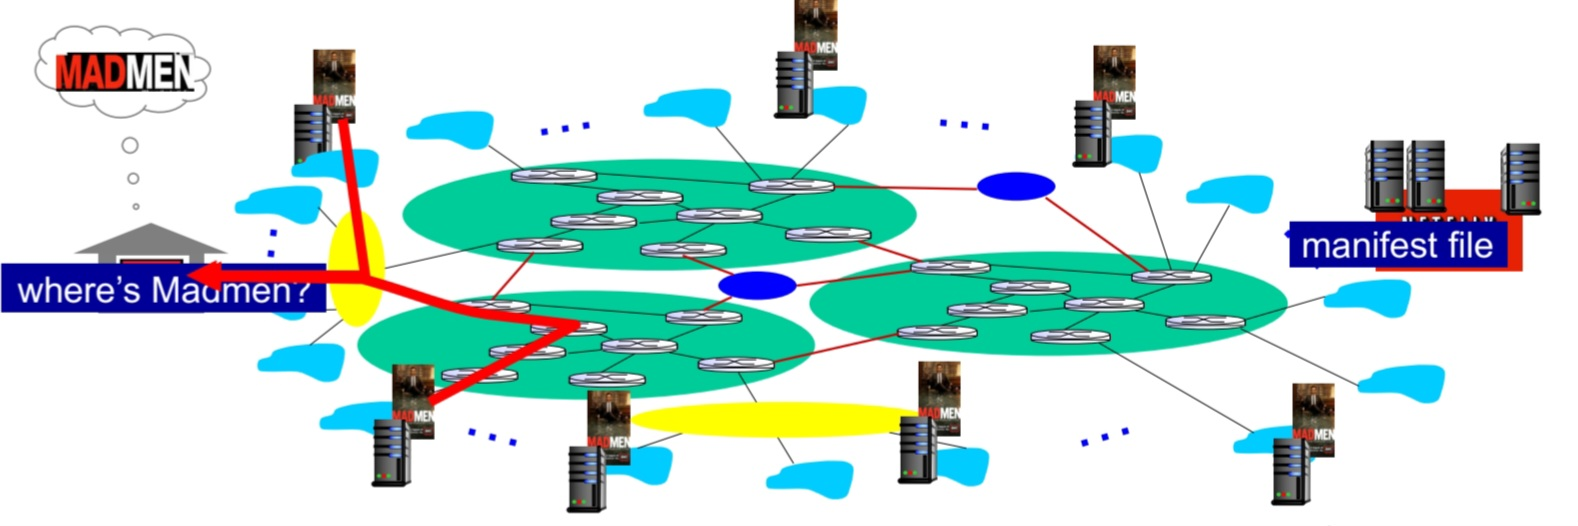
\includegraphics[width=1\linewidth]{foto reti di calcolatori/CDN_map.jpg}
    \caption{la mappa illustra visivamente il concetto fondamentale della CDN: non esiste più un unico punto di origine per il file.}
    \label{fig:placeholder}
\end{figure}

\begin{defbox}{Analisi dello Schema a Mappa}
Nell'esempio grafico (slide "Where's MadMen?"):
\begin{itemize}
    \item \textbf{Replicazione:} Il contenuto (es. la serie "MadMen") è stato copiato preventivamente su molteplici server sparsi nella rete geografica (i nodi della CDN).
    \item \textbf{Routing Intelligente:} Quando l'utente richiede "Dov'è MadMen?", la rete non lo manda a caso. La richiesta viene analizzata per trovare la copia ottimale.
    \item \textbf{Prossimità e Resilienza:}
    \begin{itemize}
        \item Normalmente, l'utente viene diretto alla copia fisicamente più \textbf{vicina} (minor latenza).
        \item Se però il percorso verso il nodo vicino è congestionato (traffico alto), la CDN è abbastanza intelligente da reindirizzare l'utente verso una copia alternativa, magari leggermente più lontana ma raggiungibile tramite un percorso libero.
    \end{itemize}
\end{itemize}

In sintesi: la mappa dimostra che la CDN trasforma Internet da un sistema "centro-periferia" a un sistema distribuito dove il contenuto "insegue" l'utente.
\end{defbox}

% ------------------------------------------------
% SEZIONE DETTAGLIO FUNZIONAMENTO CDN
% ------------------------------------------------
\newpage

\subsubsection{Accesso ai Contenuti: Il meccanismo di Reindirizzamento DNS}

Come fa un utente a collegarsi al server CDN ottimale senza conoscere il suo indirizzo IP? Il segreto risiede nell'uso intelligente del \textbf{DNS} (Domain Name System).

\begin{figure}
    \centering
    \includegraphics[width=0.5\linewidth]{}
    \label{fig:placeholder}
\end{figure}


Analizziamo il flusso di una richiesta (es. Bob vuole vedere un video su \texttt{NetCinema}) :

\begin{figure}[H]
    \centering
    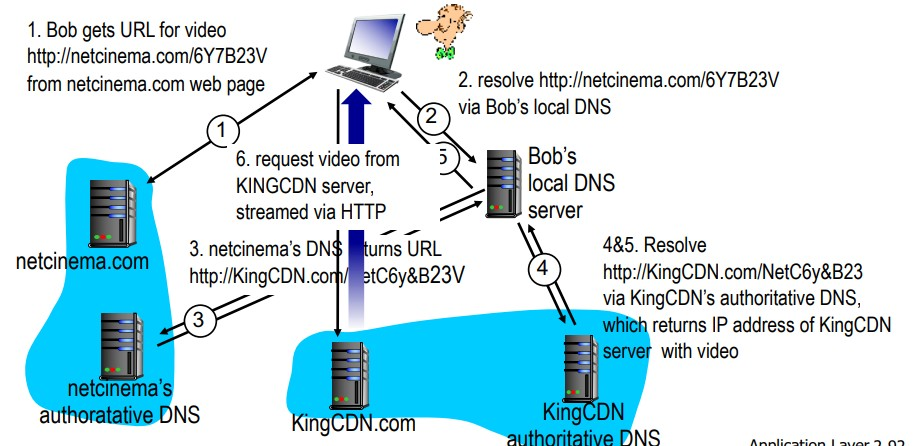
\includegraphics[width=1 \linewidth]{foto reti di calcolatori/bob.jpg}
    \caption{}
    \label{fig:placeholder}
\end{figure}

\begin{enumerate}
    \item \textbf{Richiesta Iniziale:} L'utente (Bob) naviga sul sito del provider (es. \texttt{netcinema.com}) e ottiene l'URL del video. Questo URL contiene un riferimento specifico (es. \texttt{netcinema.com/6Y7B...}).
    
    \item \textbf{Risoluzione DNS Locale:} Il computer di Bob contatta il suo server DNS locale (Local DNS) per risolvere il nome \texttt{netcinema.com}.
    
    \item \textbf{Reindirizzamento (La Chiave):} Il DNS locale contatta il DNS autoritativo di NetCinema. Qui avviene la magia: invece di restituire un indirizzo IP, il server di NetCinema restituisce un nuovo nome di dominio appartenente alla CDN (es. \texttt{KingCDN.com}). In pratica dice: \textit{"Non ho io il video, chiedi a KingCDN"}.
    
    \item \textbf{Interrogazione DNS della CDN:} Il DNS locale di Bob interroga ora il DNS autoritativo della CDN (\texttt{KingCDN}).
    
    \item \textbf{Selezione Intelligente:} Il DNS della CDN conosce la topologia della rete e l'indirizzo IP del DNS locale di Bob. Sceglie il server CDN specifico (es. a Milano o Roma) che è più vicino o meno carico e restituisce il suo indirizzo IP a Bob.
    
    \item \textbf{Streaming:} Bob contatta direttamente l'indirizzo IP ricevuto e inizia lo streaming via HTTP.
\end{enumerate}

\newpage

% ------------------------------------------------
% CASE STUDY NETFLIX (Aggiornato con slide 4)
% ------------------------------------------------

\begin{esempiobox}{Case Study: Architettura Ibrida di Netflix}

Netflix implementa questo concetto separando nettamente la logica di gestione dai server di distribuzione (CDN) .

\subsection*{1. Componenti Principali}
\begin{itemize}
    \item \textbf{Amazon Cloud (AWS):} Gestisce il "Piano di Controllo". Qui risiedono i server per la registrazione, la gestione degli account, la navigazione del catalogo e il caricamento iniziale dei video (upload delle copie multiple).
    \item \textbf{Server CDN:} Gestiscono il "Piano dei Dati". Sono i server fisici dove vengono copiate le versioni dei video per essere servite agli utenti.
\end{itemize}

\subsection*{2. Flusso Operativo (Architettura Netflix/Amazon)}
\begin{itemize}[leftmargin=*]
    \item \textbf{Fase 1 (Gestione Account):} Bob interagisce con i \textbf{server di registrazione e accounting di Netflix} per autenticarsi e gestire il proprio profilo.
    \item \textbf{Fase 2 (Navigazione e Selezione):} Bob naviga nel catalogo dei video, la cui logica è ospitata su \textbf{Amazon Cloud}. Nel frattempo, Amazon Cloud ha già provveduto a distribuire e caricare preventivamente molteplici versioni dello stesso video (a diverse risoluzioni) sui vari \textbf{server CDN} sparsi per il mondo.
    \item \textbf{Fase 3 (Manifest file):} Quando Bob seleziona un titolo, Amazon Cloud elabora la richiesta e gli restituisce un \textbf{Manifest file}. Questo file è una vera e propria "mappa" che contiene i link (URL) dei vari chunk video che puntano direttamente ai server CDN.
    \item \textbf{Fase 4 (Streaming DASH):} Il client di Bob usa il manifest per richiedere i blocchi di video direttamente al \textbf{server CDN} assegnato. Inizia così lo streaming utilizzando la tecnica \textbf{DASH}, che adatta dinamicamente la qualità in base alla banda disponibile, senza più gravare sui server centrali di Amazon.
\end{itemize}

\end{esempiobox}

\begin{figure}[H]
    \centering
    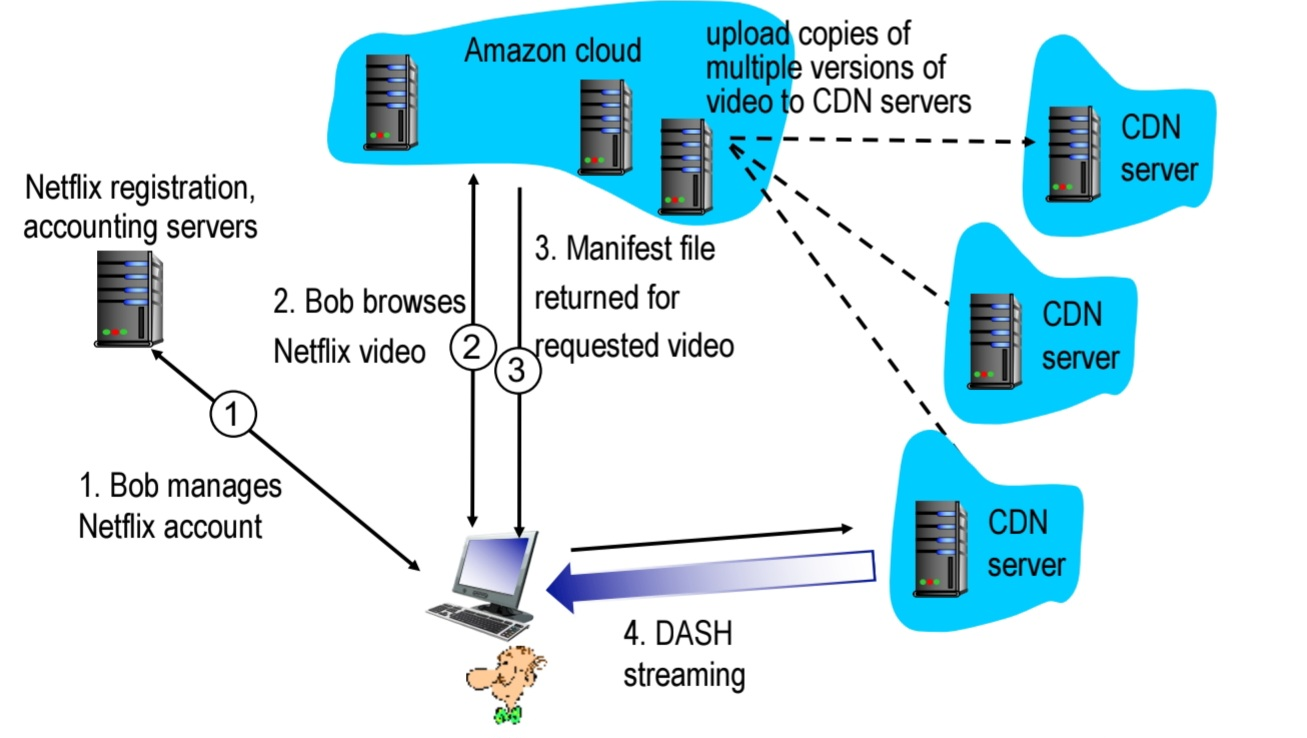
\includegraphics[width=0.7\linewidth]{foto reti di calcolatori/Netflix.jpg}
    \caption{Architettura ibrida di Netflix. Il "Piano di Controllo" (account e catalogo) è gestito da server proprietari e da Amazon Cloud, mentre il "Piano dei Dati" (lo streaming video effettivo) è delegato in modo distribuito ai server CDN.}
    \label{fig:netflix_architecture}
\end{figure}





%-------------------------------------------------
\newpage
\section{Esempio Riassuntivo: Configurazione TCP/IP di un Host Domestico}

Per concludere la panoramica sull'architettura di Internet, analizziamo cosa serve in pratica per configurare un host (es. un computer domestico) affinché possa connettersi a Internet tramite un Internet Service Provider (ISP) utilizzando un modem.

\begin{figure}[H]
    \centering
    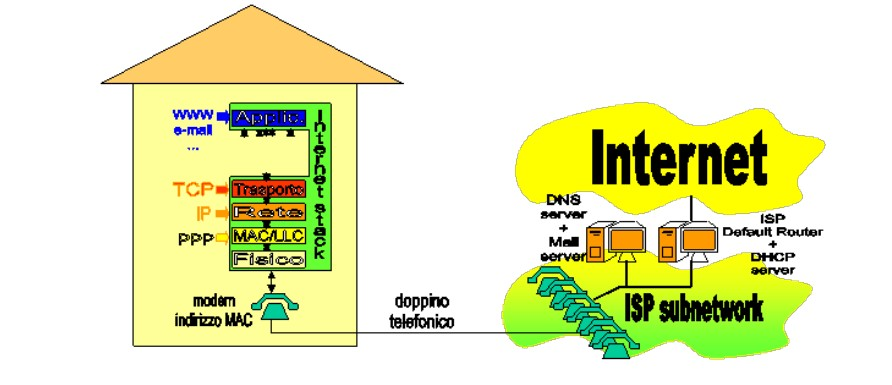
\includegraphics[width=0.8\linewidth]{foto reti di calcolatori/casa.jpg}
    \caption{Schema di collegamento di un computer domestico a Internet. Sono evidenziati i livelli della pila protocollare e i server fondamentali presenti nella sottorete dell'ISP.}
    \label{fig:config_tcp_ip}
\end{figure}

\textbf{1. Installazione e Pila Protocollare}
Per stabilire il collegamento, l'host deve innanzitutto disporre di un dispositivo hardware (scheda di rete o modem) e istanziare la pila di protocolli software:
\begin{itemize}[leftmargin=*]
    \item \textbf{Livello 1 e 2 (Fisico e MAC/LLC):} Si installa il modem, che trasmette i bit sulla linea telefonica (doppino). Al livello di collegamento (MAC/LLC) viene tipicamente adottato il protocollo \textbf{PPP} (Point-to-Point Protocol).
    \item \textbf{Livello 3 e 4 (Rete e Trasporto):} Viene istanziato lo stack \textbf{TCP/IP} fornito dal sistema operativo.
    \item \textbf{Livello 7 (Applicazione):} Vengono eseguiti i processi applicativi utili all'utente (es. HTTP per il Web, SMTP/POP3 per la posta elettronica).
    \item \textbf{Sicurezza (Opzionale):} Installazione di un firewall per impedire accessi esterni non autorizzati all'host.
\end{itemize}

\vspace{0.3cm}
\textbf{2. Informazioni di Configurazione Necessarie}
All'atto della connessione, affinché lo stack TCP/IP possa funzionare e comunicare con l'esterno, il sistema operativo deve ottenere quattro parametri fondamentali. Questi possono essere inseriti manualmente o, molto più frequentemente, ottenuti in modo automatico tramite un \textbf{Server DHCP} presente nella rete dell'ISP:

\begin{enumerate}[leftmargin=*]
    \item \textbf{Indirizzo IP dell'host:} Un indirizzo valido e univoco relativo alla sottorete gestita dall'ISP.
    \item \textbf{Maschera di rete (Netmask):} Per distinguere la parte di rete dalla parte di host.
    \item \textbf{Default Router (Gateway):} L'indirizzo IP del router dell'ISP a cui inviare tutto il traffico destinato al resto di Internet.
    \item \textbf{Server DNS:} L'indirizzo IP del server a cui rivolgere le query per tradurre i nomi di dominio (es. www.google.com) in indirizzi IP.
\end{enumerate}

Possono inoltre essere configurati gli indirizzi IP di servizi applicativi specifici forniti dall'ISP, come i server di posta elettronica (SMTP, POP3, IMAP).

\begin{notebox}{\textbf{Ciclo di vita della connessione}}
Nel momento in cui l'host domestico si disconnette (rilascio della comunicazione), il server DHCP dell'ISP cancella dinamicamente l'assegnazione dell'indirizzo IP. Questo indirizzo tornerà nel \textit{pool} delle risorse disponibili e verrà eventualmente riciclato per essere assegnato a un altro dispositivo che ne farà richiesta.
\end{notebox}

\section{Schema Riassuntivo Finale: Livelli, Indirizzi e Dispositivi}

Per padroneggiare l'architettura delle reti, è fondamentale avere ben chiara la corrispondenza tra i livelli dello stack, i dispositivi che vi operano, gli indirizzi utilizzati e il nome corretto dell'unità di dati a quel livello (\textbf{PDU} - \textit{Protocol Data Unit}).

\vspace{0.3cm}

\begin{table}[H]
\centering
\renewcommand{\arraystretch}{1.5} % Aumenta leggermente lo spazio tra le righe
\begin{tabular}{|c|p{3.2cm}|p{3.2cm}|p{2.8cm}|p{3.2cm}|}
\hline

\textbf{Livello} & \textbf{PDU (Unità Dati)} & \textbf{Indirizzamento} & \textbf{Dispositivi} & \textbf{Protocolli Chiave} \\
\hline
\textbf{5. Applicazione} & Messaggio / Dati \newline \textit{(Payload)} & URL, Nomi a dominio, Indirizzi Email & Host (Client/Server), Proxy Cache & HTTP, SMTP, DNS, DHCP, POP3  \\
\hline
\textbf{4. Trasporto} & Segmento (TCP) / Datagramma (UDP) & Numero di Porta \newline \textit{(es. 80, 25, 443)} & Host, Firewall & TCP, UDP  \\
\hline
\textbf{3. Rete} & Pacchetto \newline \textit{(Datagramma IP)} & Indirizzo IP logico \newline \textit{(es. 192.168.1.1)} & Router & IPv4, IPv6, ICMP, ARP  \\
\hline
\textbf{2. MAC/LLC} & Frame \newline \textit{(Trama)} & Indirizzo MAC fisico \newline \textit{(es. 00:1A:2B...)} & Switch, Bridge & Ethernet, Wi-Fi (802.11)  , Token Ring \\
\hline
\textbf{1. Fisico} & Bit \newline \textit{(Segnale elettrico/ottico)} & Nessuno & Hub, Repeater, Modem, Cavi & (Standard fisici vari)  \\
\hline
\end{tabular}
\caption{Cheat Sheet dei livelli di rete: corrispondenza tra PDU, indirizzamento, apparati hardware e protocolli.}
\label{tab:riassunto_livelli_stack}
\end{table}


\end{document}